% Conversion LaTeX du fichier Word "2-ModelisationMecanismes2022.docx"
% Images extraites dans le dossier ./images
% Fichier prévu pour être inclus dans votre projet kaobook / cours existant.
% Packages nécessaires dans le préambule principal : graphicx, xcolor, hyperref, longtable, booktabs, array, calc, multirow, ulem.

\graphicspath{{images/}}
\providecommand{\ul}[1]{\uline{#1}}

\setchapterimage{../Style/FondPoly.png}
\setchapterpreamble[u]{\margintoc}

\begingroup
\definecolor{kaoblue}{RGB}{0,82,155}
\addtokomafont{chapter}{\color{kaoblue}}
\chapter*{Modélisation des Mécanismes}
\endgroup
\setcounter{chapter}{2}


\includegraphics[width=\linewidth]{images/image1.png}

\textbf{Sciences Industrielles pour L'Ingénieur}


\includegraphics[width=\linewidth]{images/image3.png}

Cycle 2 : Modéliser et déterminer les lois de mouvement d'un mécanisme

\textbf{Modélisation des Mécanismes}

Thomas Lusseau

Lycée Robert Doisneau - ATS

%\tableofcontents
\clearpage

\section*{Objectifs du cours}

Modéliser et savoir analyser le comportement cinématique d'un mécanisme
avec un schéma cinématique et/ou un graphe de liaisons.

Savoirs

\textbf{Je connais~:}

\begin{longtable}[]{@{}
  >{\raggedright\arraybackslash}p{(\columnwidth - 2\tabcolsep) * \real{0.9045}}
  >{\raggedright\arraybackslash}p{(\columnwidth - 2\tabcolsep) * \real{0.0955}}@{}}
\toprule\noalign{}
\begin{minipage}[b]{\linewidth}\raggedright
\begin{itemize}
\item
  les noms des dix liaisons usuelles~;
\end{itemize}
\end{minipage} & \begin{minipage}[b]{\linewidth}\raggedright
⃝
\end{minipage} \\
\midrule\noalign{}
\endhead
\bottomrule\noalign{}
\endlastfoot
\begin{minipage}[t]{\linewidth}\raggedright
\begin{itemize}
\item
  les symboles de représentation 2D et 3D des dix liaisons usuelles~;
\end{itemize}
\end{minipage} & ⃝ \\
\begin{minipage}[t]{\linewidth}\raggedright
\begin{itemize}
\item
  la forme générale des torseurs cinématiques associés aux dix liaisons
  usuelles~;
\end{itemize}
\end{minipage} & ⃝ \\
\begin{minipage}[t]{\linewidth}\raggedright
\begin{itemize}
\item
  les symboles permettant de représenter les transmetteurs usuels~;
\end{itemize}
\end{minipage} & ⃝ \\
\begin{minipage}[t]{\linewidth}\raggedright
\begin{itemize}
\item
  les différentes liaisons permettant de modéliser le comportement
  cinématique entre deux Classes d'Equivalence Cinématique (CEC) en
  contact par l'intermédiaire de roulements~;
\end{itemize}
\end{minipage} & ⃝ \\
\begin{minipage}[t]{\linewidth}\raggedright
\begin{itemize}
\item
  la démarche (différentes étapes) pour obtenir un schéma cinématique.
\end{itemize}
\end{minipage} & ⃝ \\
\end{longtable}

Savoir-faire

\textbf{Je sais~:}

\begin{longtable}[]{@{}
  >{\raggedright\arraybackslash}p{(\columnwidth - 2\tabcolsep) * \real{0.9045}}
  >{\raggedright\arraybackslash}p{(\columnwidth - 2\tabcolsep) * \real{0.0955}}@{}}
\toprule\noalign{}
\begin{minipage}[b]{\linewidth}\raggedright
\begin{itemize}
\item
  Identifier une liaison usuelle sur un schéma cinématique et la
  caractériser par son nom, sa description géométrique, ses degrés de
  liberté~et son torseur cinématique~;
\end{itemize}
\end{minipage} & \begin{minipage}[b]{\linewidth}\raggedright
⃝
\end{minipage} \\
\midrule\noalign{}
\endhead
\bottomrule\noalign{}
\endlastfoot
\begin{minipage}[t]{\linewidth}\raggedright
\begin{itemize}
\item
  repérer les Classes d'Equivalence Cinématique (CEC) sur la
  représentation technique 2D ou 3D d'un système~;
\end{itemize}
\end{minipage} & ⃝ \\
\begin{minipage}[t]{\linewidth}\raggedright
\begin{itemize}
\item
  identifier la géométrie du contact entre deux pièces~;
\end{itemize}
\end{minipage} & ⃝ \\
\begin{minipage}[t]{\linewidth}\raggedright
\begin{itemize}
\item
  identifier le mouvement relatif entre deux ~CEC en contact et le
  modéliser par une des dix liaisons usuelles~;
\end{itemize}
\end{minipage} & ⃝ \\
\begin{minipage}[t]{\linewidth}\raggedright
\begin{itemize}
\item
  réaliser un graphe des liaisons~;
\end{itemize}
\end{minipage} & ⃝ \\
\begin{minipage}[t]{\linewidth}\raggedright
\begin{itemize}
\item
  élaborer un schéma cinématique~;
\end{itemize}
\end{minipage} & ⃝ \\
\begin{minipage}[t]{\linewidth}\raggedright
\begin{itemize}
\item
  déterminer la liaison équivalente à plusieurs liaisons en série et/ou
  en parallèle pour obtenir un schéma cinématique minimal.
\end{itemize}
\end{minipage} & ⃝ \\
\end{longtable}

\section{MISE EN SITUATION}\label{mise-en-situation}

\subsection{Cas n°1~: Lenteur d'un robot de
chirurgie}\label{cas-n1-lenteur-dun-robot-de-chirurgie}

Même si elle n'est pas encore aussi répandue en France qu'aux
Etats-Unis, la chirurgie robotique se développe peu à peu. Son usage
nécessite la maîtrise de la machine et une familiarisation avec sa
manipulation, mais aussi une prise en compte des contraintes qu'elle
impose, notamment sur la durée de l'intervention. L'absence de
précautions particulières peut être source de responsabilité. C'est ce
que rappelle un arrêt de la cour administrative d'appel de Lyon du 29
septembre 2016.

Il apparaît ainsi que l'usage du robot est en lien de causalité direct
et certain avec les dommages du fait de l'allongement de la durée de
l'intervention, due à la fois aux nécessités d'installation du robot et
à son maniement « hésitant » par l'opérateur.


\includegraphics[width=\linewidth]{images/image5.jpeg}

Pour des nombreux systèmes, en particulier pour ceux du domaine de la
robotique industrielle ou grand public, un des principaux enjeux de leur
concepteur est de faire en sorte qu'ils respectent parfaitement la
\textbf{cinématique} imposée par leur cahier des charges. Il s'agit de
s'assurer que les \textbf{mouvements} des pièces qui les constituent
s'exécutent parfaitement suivant des \textbf{directions} et à des
\textbf{vitesses maitrisées}.

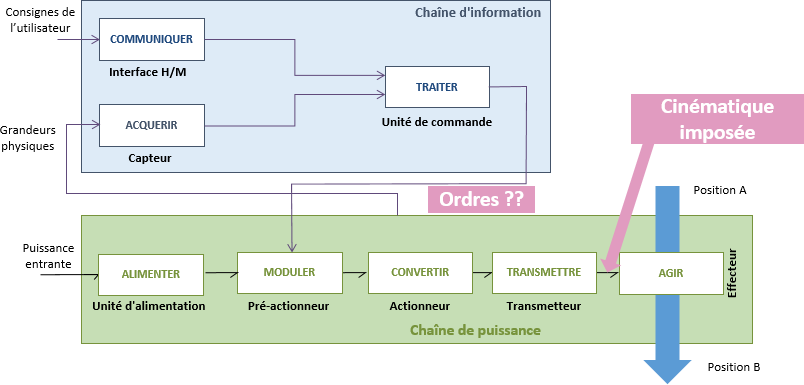
\includegraphics[width=\linewidth]{images/image6.png}On
parle alors des \textbf{lois de commande en mouvement} d'un
\textbf{mécanisme} qui doivent permettre, comme finalité, d'établir des
\textbf{relations} entre les \textbf{ordres} envoyés par l'unité de
commande aux pré-actionneurs des chaînes d'énergie- puissance et la
\textbf{cinématique imposée aux effecteurs} par le cahier des charges du
système.

\subsection[Cas n°2~: Prothèse
transtibiale]{\texorpdfstring{\protect
\includegraphics[width=\linewidth]{images/image7.jpeg}Cas
n°2~: Prothèse
transtibiale}{Cas n°2~: Prothèse transtibiale}}\label{cas-n2-prothuxe8se-transtibiale}

La prothèse transtibiale doit permettre à la personne de réaliser les
mêmes mouvements qu'un pied réel, que ce soit en termes d'amplitudes, de
vitesse ou d'accélération.

Pour maitriser les positions et les vitesses, il faut pouvoir modéliser
les différents mouvements du mécanisme~!

'\,'

\section{~INTRODUCTION A LA MODELISATION
CINEMATIQUE}\label{introduction-a-la-modelisation-cinematique}

\subsection{Définitions et
hypothèses}\label{duxe9finitions-et-hypothuxe8ses}

\textbf{Mécanisme}~: C'est l'ensemble des solides de la chaîne de
puissance situées entre l'actionneur et l'effecteur, qui permet le
transfert de puissance mécanique.

\emph{Source : ISO 15288.}

\textbf{Définition}

\textbf{Solide (ou CEC)}~: Une pièce ou un ensemble de pièces qui sont
assemblées entre elles (collées, soudées, vissées, \ldots) et qui sont
cinématiquement liées (i.e même mouvement), est appelé solide (ou Classe
d'Equivalence Cinématique).

\textbf{Définition}

Lors de l'utilisation d'un mécanisme, les solides qui le constituent se
déforment sous l'action des efforts qu'ils subissent. Cette année, nous
ferons l'hypothèse que ces déformations sont suffisamment petites pour
que l'on puisse les négliger et on considérera les solides
indéformables. S'ils sont considérés déformables, cela fait l'objet de
la Résistance Des Matériaux (RDM) mais qui n'est pas au programme en
ATS.

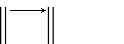
\includegraphics[width=\linewidth]{images/image10.png}Un
\textbf{solide indéformable} (S) est tel que les \textbf{distances}
entre tous les couples de \textbf{points matériels} ne varient pas au
cours du temps : ∀\emph{t}, ∀\emph{A}, \emph{B}∈\emph{S}, \emph{AB} =
Constante

\begin{quote}
Cette hypothèse n'est pas valable pour les pièces dont la fonction est
précisément de se déformer tels que les ressorts, barres de torsion,
\ldots{}
\end{quote}

\subsection{Modèle cinématique}\label{moduxe8le-cinuxe9matique}

Lorsque l'on souhaite étudier le comportement cinématique d'un
mécanisme, il est nécessaire de s'appuyer sur modèle cinématique. Ce
modèle est en général un \emph{schéma cinématique} et/ou un \emph{graphe
des liaisons}.

\begin{quote}
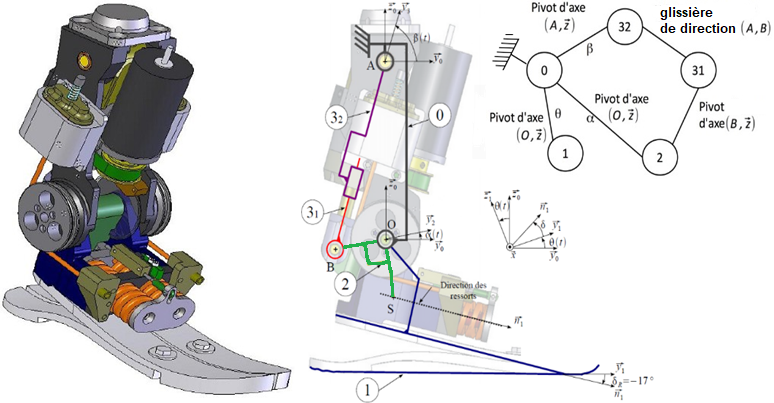
\includegraphics[width=\linewidth]{images/image12.png}
\end{quote}

\begin{longtable}[]{@{}
  >{\raggedright\arraybackslash}p{(\columnwidth - 2\tabcolsep) * \real{0.3600}}
  >{\raggedright\arraybackslash}p{(\columnwidth - 2\tabcolsep) * \real{0.6400}}@{}}
\toprule\noalign{}
\begin{minipage}[b]{\linewidth}\raggedright
\begin{quote}
\emph{Prothèse transtibiale}
\end{quote}
\end{minipage} & \begin{minipage}[b]{\linewidth}\raggedright
\emph{schéma cinématique (2D) et graphe des liaisons}
\end{minipage} \\
\midrule\noalign{}
\endhead
\bottomrule\noalign{}
\endlastfoot
\end{longtable}

Ces représentations schématiques simplifiées du mécanisme réel sont
utilisées en \emph{phase d'analyse} d'un système existant ou en
\emph{phase de conception} d'un nouveau système et sont des outils de
communication scientifique efficaces.

\subsection{Schéma cinématique d'un
mécanisme}\label{schuxe9ma-cinuxe9matique-dun-muxe9canisme}

Un schéma cinématique propose une représentation géométrique d'un modèle
cinématique. Il spécifie les mouvements possibles entre les solides,
appelées liaisons et les positions relatives de ces liaisons dans
l'espace.

Dans un schéma cinématique :

\begin{itemize}
\item
  les liaisons entre les solides sont représentées par des symboles
  normalisés ;
\item
  les solides sont représentés par des traits reliant ces symboles.
\end{itemize}

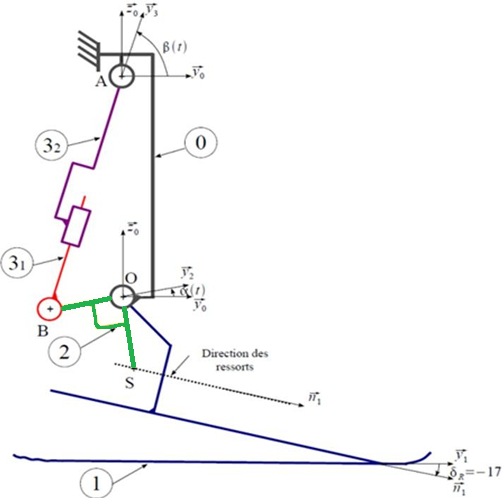
\includegraphics[width=\linewidth]{images/image13.png}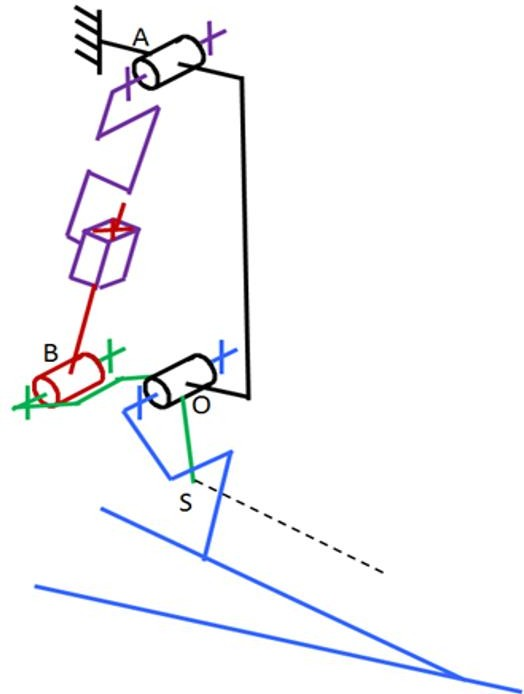
\includegraphics[width=\linewidth]{images/image14.jpeg}

\begin{longtable}[]{@{}
  >{\raggedright\arraybackslash}p{(\columnwidth - 2\tabcolsep) * \real{0.5000}}
  >{\raggedright\arraybackslash}p{(\columnwidth - 2\tabcolsep) * \real{0.5000}}@{}}
\toprule\noalign{}
\begin{minipage}[b]{\linewidth}\raggedright
\begin{quote}
\emph{Schéma cinématique 3D}
\end{quote}
\end{minipage} & \begin{minipage}[b]{\linewidth}\raggedright
\emph{Schéma cinématique 2D}
\end{minipage} \\
\midrule\noalign{}
\endhead
\bottomrule\noalign{}
\endlastfoot
\end{longtable}

\begin{quote}
Le schéma est dessiné en deux dimensions (schéma plan) ou trois
dimensions (schéma en perspective). En plus des symboles et traits de
définition des solides, on y trouve des points, des vecteurs et des
droites.
\end{quote}

Une liaison entre deux solides a toujours exactement deux couleurs~!

'\,'

\subsection{Graphe de liaison d'un
mécanisme}\label{graphe-de-liaison-dun-muxe9canisme}

Un graphe des liaisons propose une représentation graphique d'un modèle
cinématique.

\begin{quote}
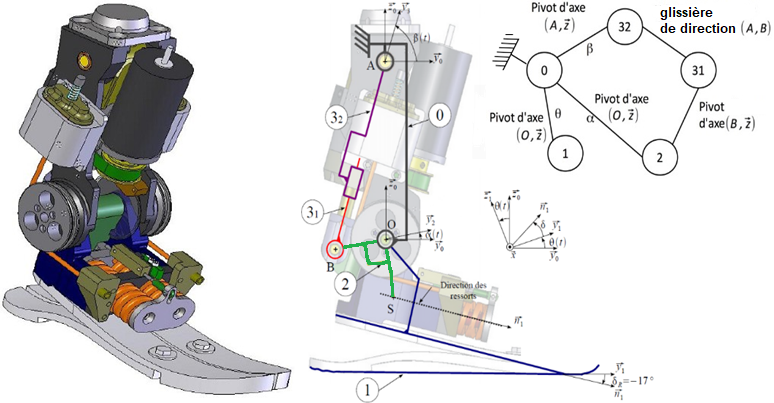
\includegraphics[width=\linewidth]{images/image12.png}
\end{quote}

\begin{longtable}[]{@{}
  >{\raggedright\arraybackslash}p{(\columnwidth - 2\tabcolsep) * \real{0.3600}}
  >{\raggedright\arraybackslash}p{(\columnwidth - 2\tabcolsep) * \real{0.6400}}@{}}
\toprule\noalign{}
\begin{minipage}[b]{\linewidth}\raggedright
\begin{quote}
\emph{Prothèse transtibiale}
\end{quote}
\end{minipage} & \begin{minipage}[b]{\linewidth}\raggedright
\emph{schéma cinématique (2D) et graphe des liaisons}
\end{minipage} \\
\midrule\noalign{}
\endhead
\bottomrule\noalign{}
\endlastfoot
\end{longtable}

Le graphe des liaisons est graphiquement plus simple à réaliser qu'un
schéma cinématique car la géométrie n'est pas représentée.

\begin{quote}
Dans un graphe des liaisons :
\end{quote}

\begin{itemize}
\item
  les \textbf{solides} sont les \textbf{nœuds} du graphe ;
\item
  les \textbf{liaisons} entre les solides sont représentées par les
  \textbf{arrêtes} du graphe le long desquelles on indique les
  \textbf{caractéristiques géométriques} de la liaison.
\end{itemize}

Mais il n'y a pas plus d'informations dans un schéma cinématique que
dans le graphe des liaisons qui lui est associé. Il s'agit de
\textbf{deux représentations d'un même modèle de comportement
cinématique}, mais qui mettent en avant des informations différentes.

Toujours penser à bien repérer le bâti, qui est la pièce référence du
mécanisme. Cela est utile lors de la détermination des actions
mécaniques (on n'isole pas le bâti).

'\,'

\paragraph*{Chaîne de solides ouverte, fermée et
complexe}\label{chauxeene-de-solides-ouverte-fermuxe9e-et-complexe}
\addcontentsline{toc}{paragraph}{Chaîne de solides ouverte, fermée et
complexe}

Parfois, au lieu de dire graphe de liaisons, le terme «~chaine de
solides~» est utilisé. Cette chaîne de solide peut apparaître sous
différente forme après la modélisation. On les classe sous trois types~:
les chaines ouvertes, les chaines fermées et les chaines complexes.
Suivant le type de chaine de solides, la méthode pour déterminer la loi
entrée sortie sera différente.

\begin{longtable}[]{@{}
  >{\raggedright\arraybackslash}p{(\columnwidth - 4\tabcolsep) * \real{0.3197}}
  >{\raggedright\arraybackslash}p{(\columnwidth - 4\tabcolsep) * \real{0.3138}}
  >{\raggedright\arraybackslash}p{(\columnwidth - 4\tabcolsep) * \real{0.3666}}@{}}
\toprule\noalign{}
\begin{minipage}[b]{\linewidth}\raggedright
\textbf{Chaîne ouverte}
\end{minipage} & \begin{minipage}[b]{\linewidth}\raggedright
\textbf{Chaîne fermée}
\end{minipage} & \begin{minipage}[b]{\linewidth}\raggedright
\textbf{Chaîne complexe}
\end{minipage} \\
\midrule\noalign{}
\endhead
\bottomrule\noalign{}
\endlastfoot
Une chaîne de solides 0, 1, 2\ldots{} est ouverte si les solides des
extrêmes sont différents. & Une chaîne de solides 0, 1, 2\ldots{} est
fermée si le solide initial est le même que le solide final. & Une
chaîne de solides 0, 1, 2\ldots{} est complexe si elle comporte
plusieurs chaînes ouvertes ou fermées. \\

\includegraphics[width=\linewidth]{images/image15.png}

L'exemple type est le robot~:

Le premier solide étant le bâti et le dernier, la pince.

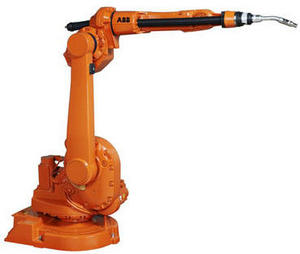
\includegraphics[width=\linewidth]{images/image16.jpeg}
&

\includegraphics[width=\linewidth]{images/image15.png}

Exemple~: antenne de radar

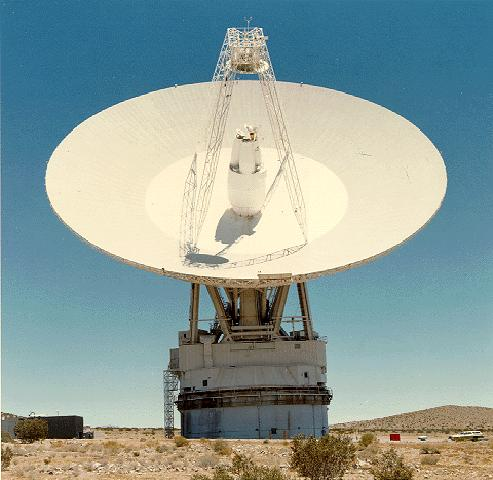
\includegraphics[width=\linewidth]{images/image17.jpeg}
&

\includegraphics[width=\linewidth]{images/image15.png}

Exemple~: simulateur de vol

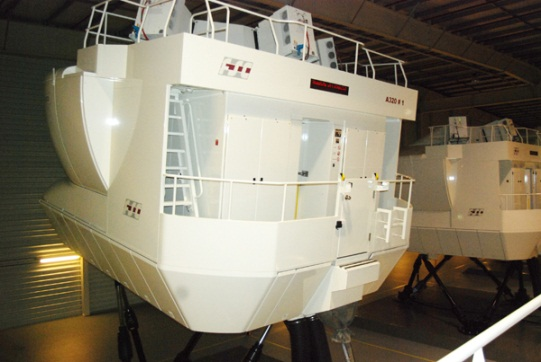
\includegraphics[width=\linewidth]{images/image18.jpeg} \\
\end{longtable}

\section{LES LIAISONS CINEMATIQUES}\label{les-liaisons-cinematiques}

\subsection{Introduction}\label{introduction}

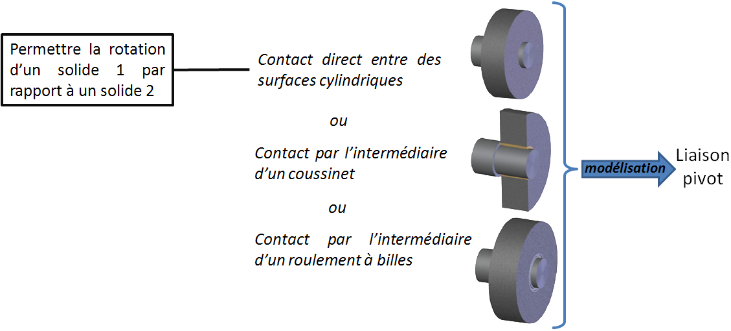
\includegraphics[width=\linewidth]{images/image19.png}Une
liaison est un \emph{\textbf{modèle du comportement cinématique}} d'un
solide par rapport à un autre. Elle permet de définir les possibilités
de mouvement entre deux solides en contact (direct ou par
l'intermédiaire d'éléments de guidage interposés (roulements,
coussinets\ldots), indépendamment de sa réalisation matérielle. Cela
signifie que \emph{\textbf{différentes réalités technologiques}} peuvent
conduire au même comportement cinématique et donc à la
\emph{\textbf{même liaison}}.

\subsection{Degrés de liberté}\label{degruxe9s-de-libertuxe9}

\textbf{Degré de liberté}~: chacun des \textbf{\emph{mouvements relatifs
élémentaires indépendants}} (le mouvement relatif d'un solide par
rapport à l'autre peut avoir lieu indépendamment des autres mouvements
possibles) autorisés par une liaison. Ils correspondent aux
\emph{\textbf{rotations}} et \emph{\textbf{translations relatives}}
suivant les axes de la base locale associée à la liaison.

\textbf{Définition}

\begin{longtable}[]{@{}
  >{\raggedright\arraybackslash}p{(\columnwidth - 4\tabcolsep) * \real{0.0960}}
  >{\raggedright\arraybackslash}p{(\columnwidth - 4\tabcolsep) * \real{0.6496}}
  >{\raggedright\arraybackslash}p{(\columnwidth - 4\tabcolsep) * \real{0.2544}}@{}}
\toprule\noalign{}
\multirow{3}{=}{\begin{minipage}[b]{\linewidth}\raggedright
\begin{quote}
\emph{\textbf{3 degrés de liberté en translation}}
\end{quote}
\end{minipage}} &
\multicolumn{2}{>{\raggedright\arraybackslash}p{(\columnwidth - 4\tabcolsep) * \real{0.9040} + 2\tabcolsep}@{}}{%
\begin{minipage}[b]{\linewidth}\raggedright
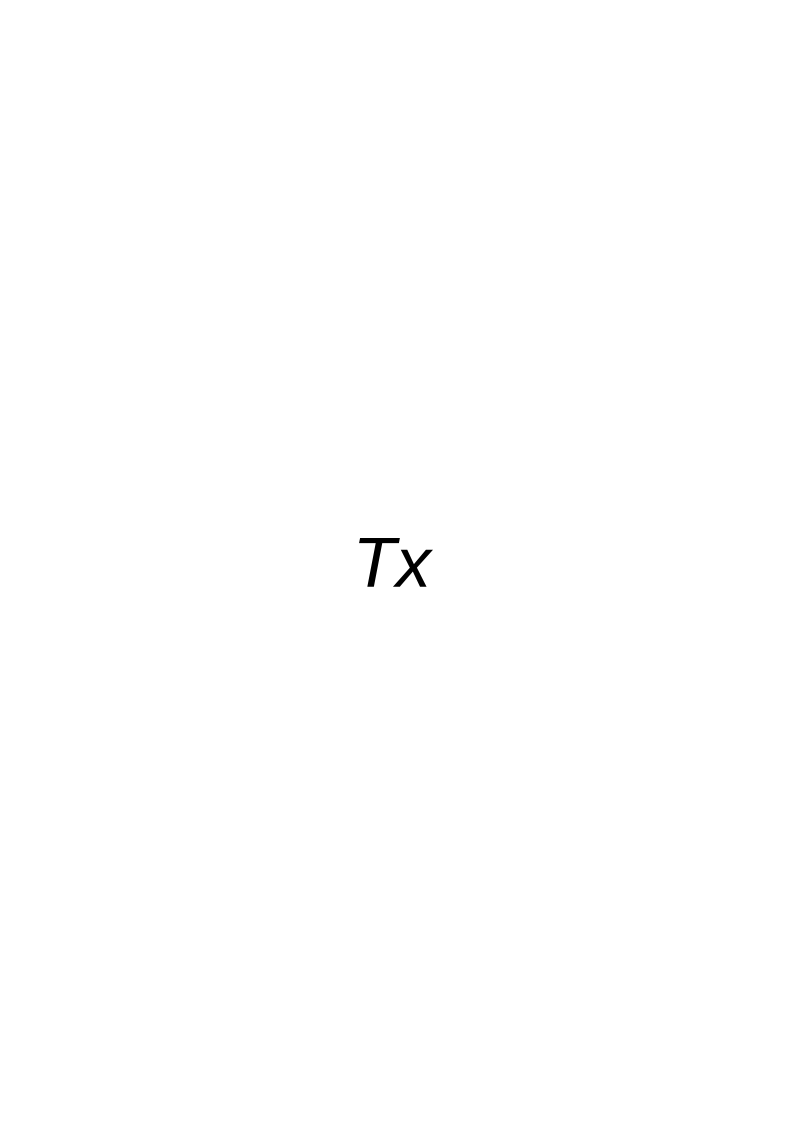
\includegraphics{images/image20.png} = liberté de mouvement de
translation rectiligne de direction
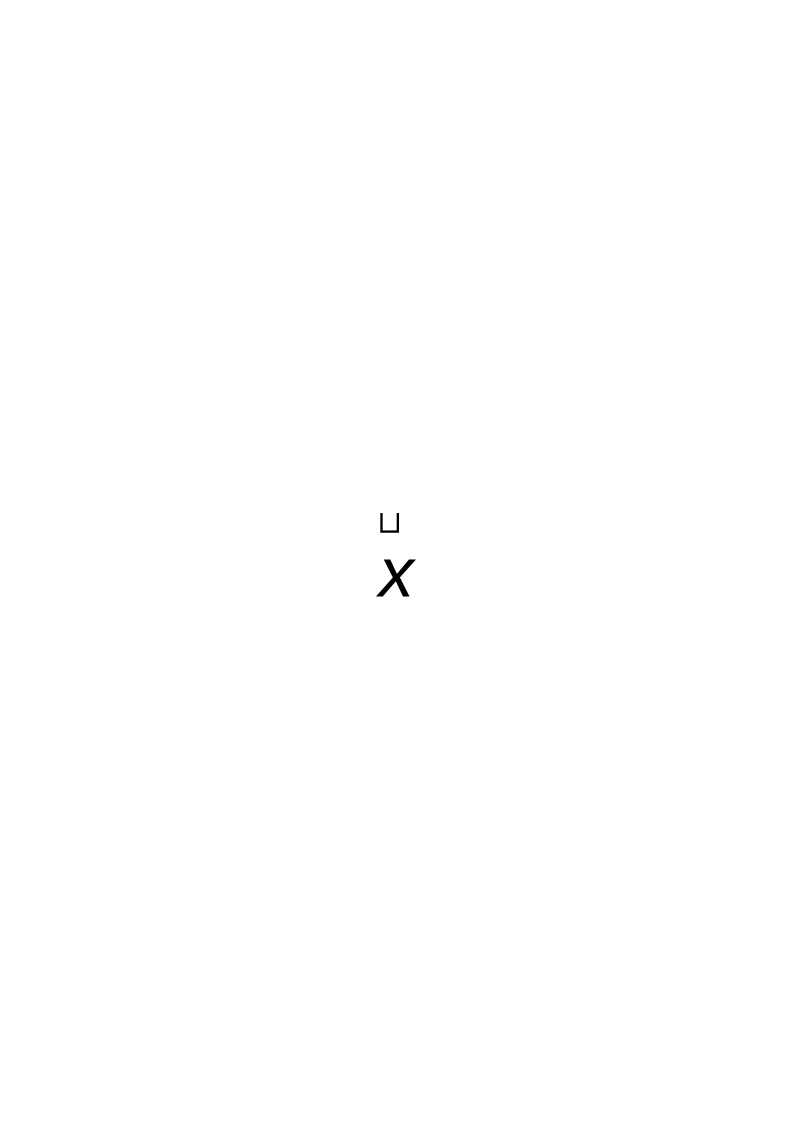
\includegraphics{images/image21.png}
\end{minipage}} \\
&
\multicolumn{2}{>{\raggedright\arraybackslash}p{(\columnwidth - 4\tabcolsep) * \real{0.9040} + 2\tabcolsep}@{}}{%
\begin{minipage}[b]{\linewidth}\raggedright
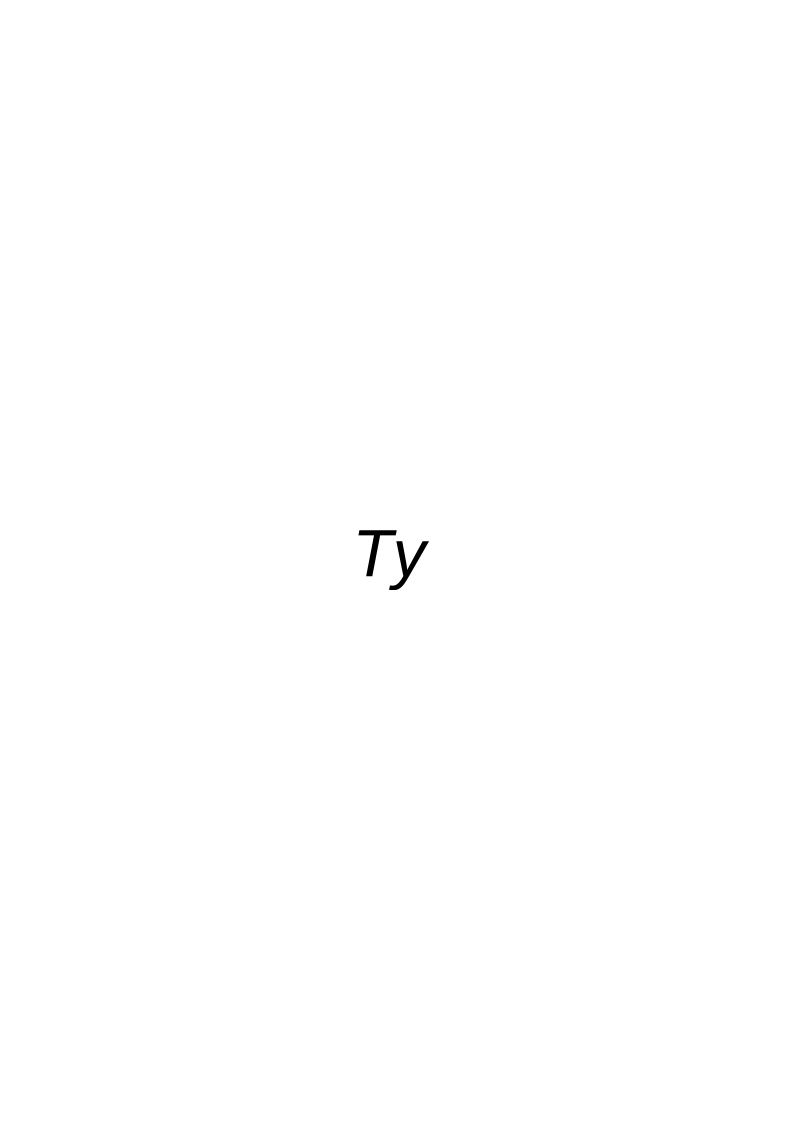
\includegraphics{images/image22.png} = liberté de mouvement de
translation rectiligne de direction
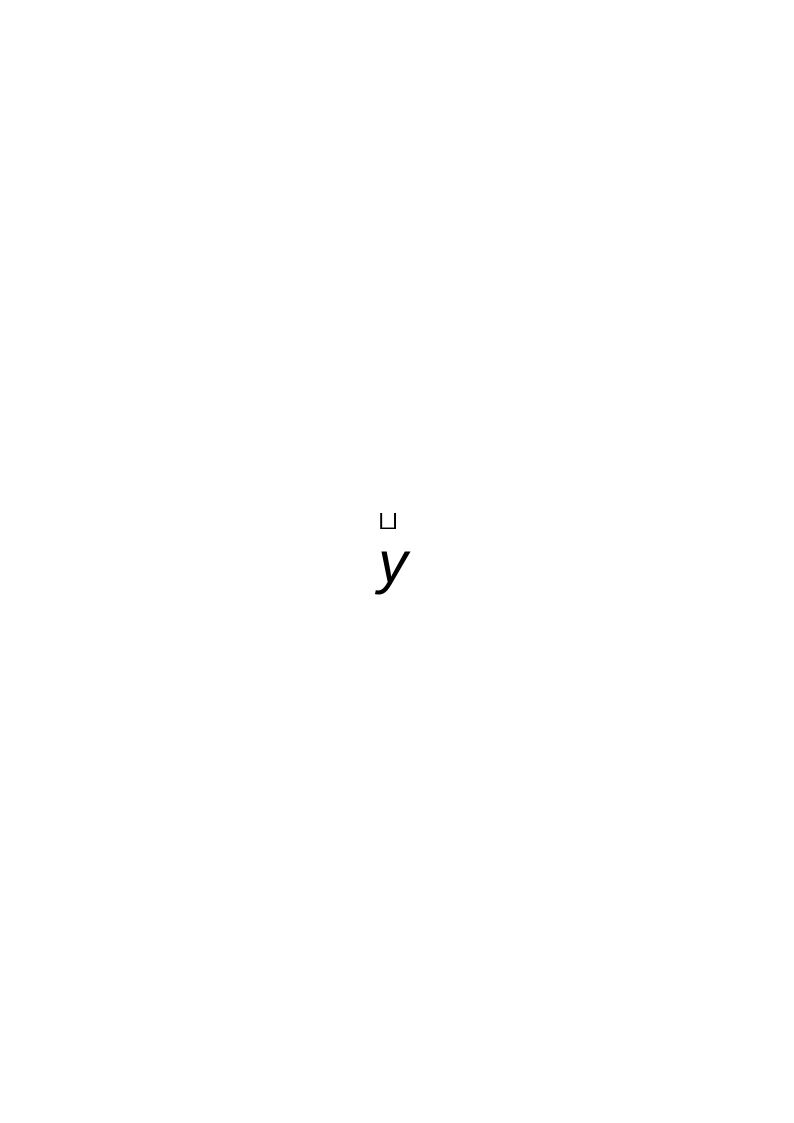
\includegraphics{images/image23.png}
\end{minipage}} \\
& \begin{minipage}[b]{\linewidth}\raggedright
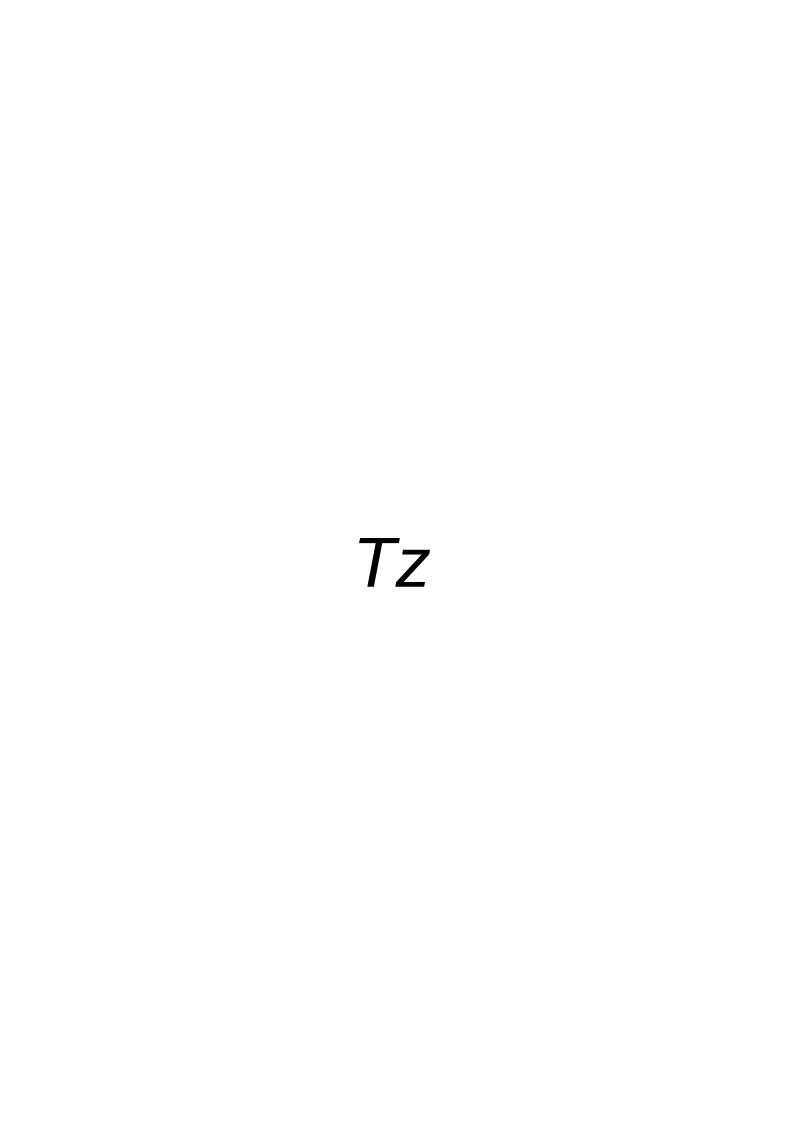
\includegraphics{images/image24.png} = liberté de mouvement de
translation rectiligne de direction
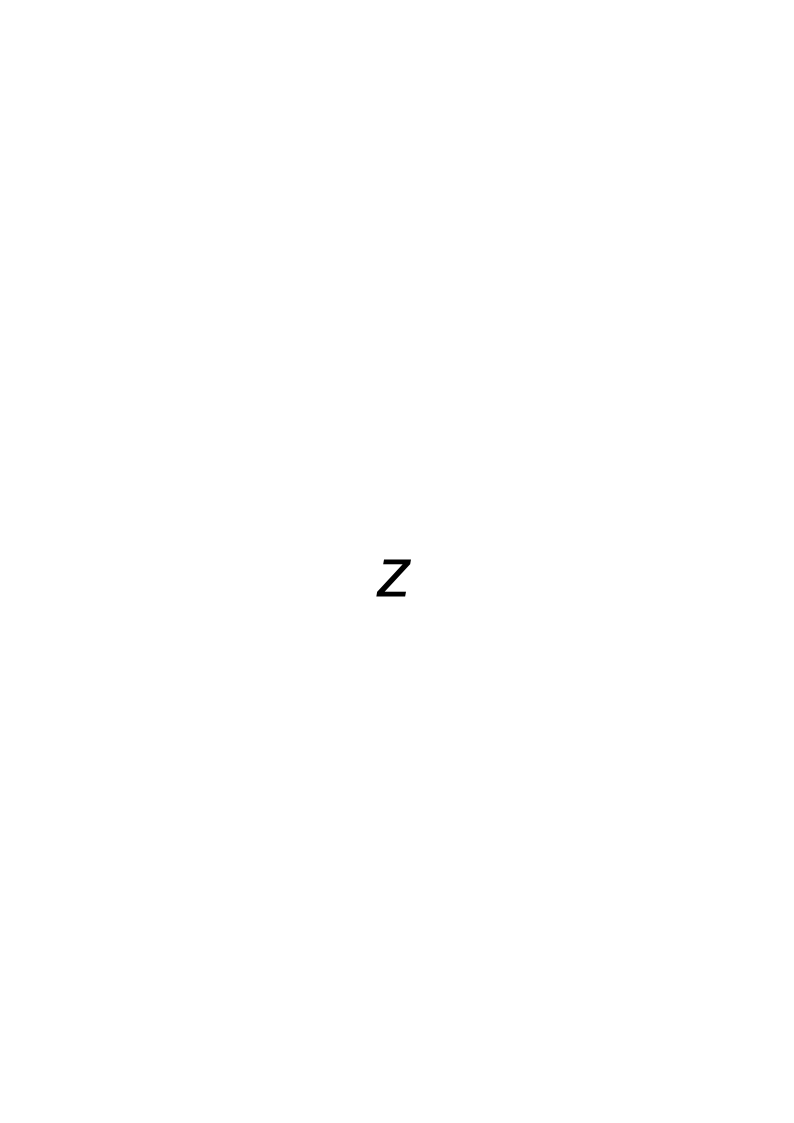
\includegraphics{images/image25.png}
\end{minipage} &
\multirow{4}{=}{\begin{minipage}[b]{\linewidth}\raggedright

\includegraphics[width=\linewidth]{images/image26.png}
\end{minipage}} \\
\multirow{3}{=}{\begin{minipage}[b]{\linewidth}\raggedright
\begin{quote}
\emph{\textbf{3 degrés de liberté en rotation}}
\end{quote}
\end{minipage}} & \begin{minipage}[b]{\linewidth}\raggedright
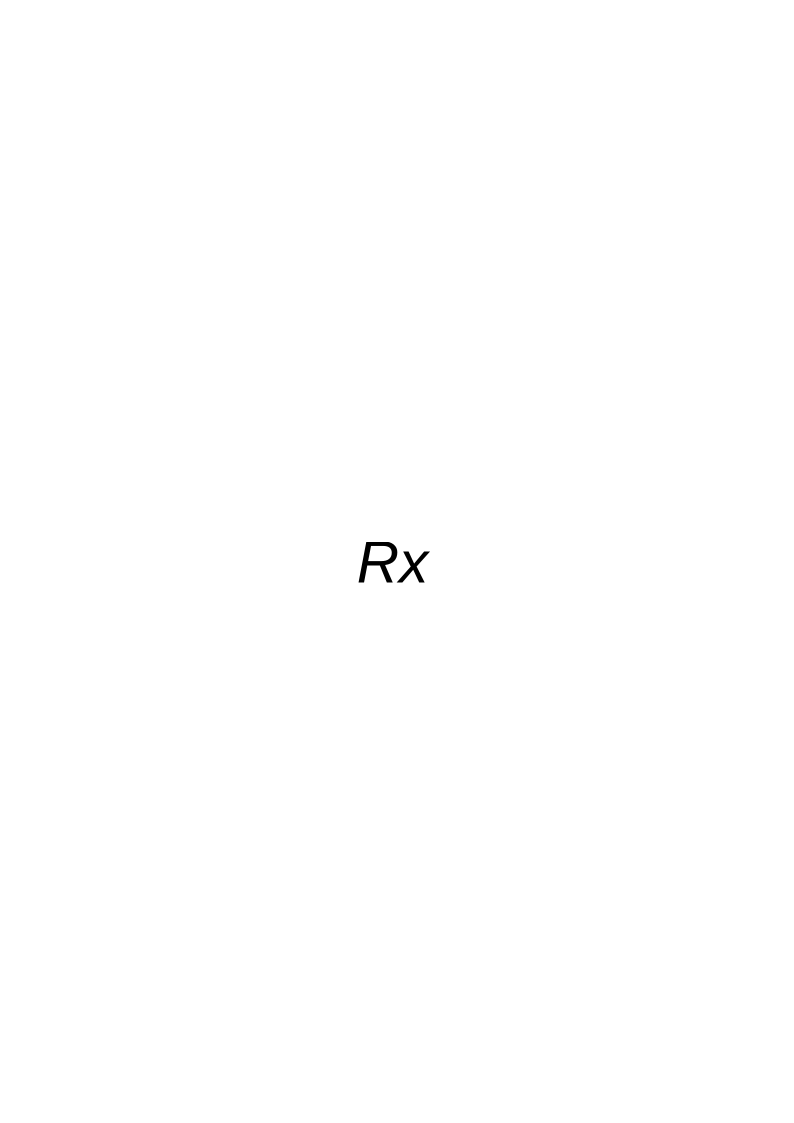
\includegraphics{images/image27.png} = liberté de mouvement de rotation
d'axe 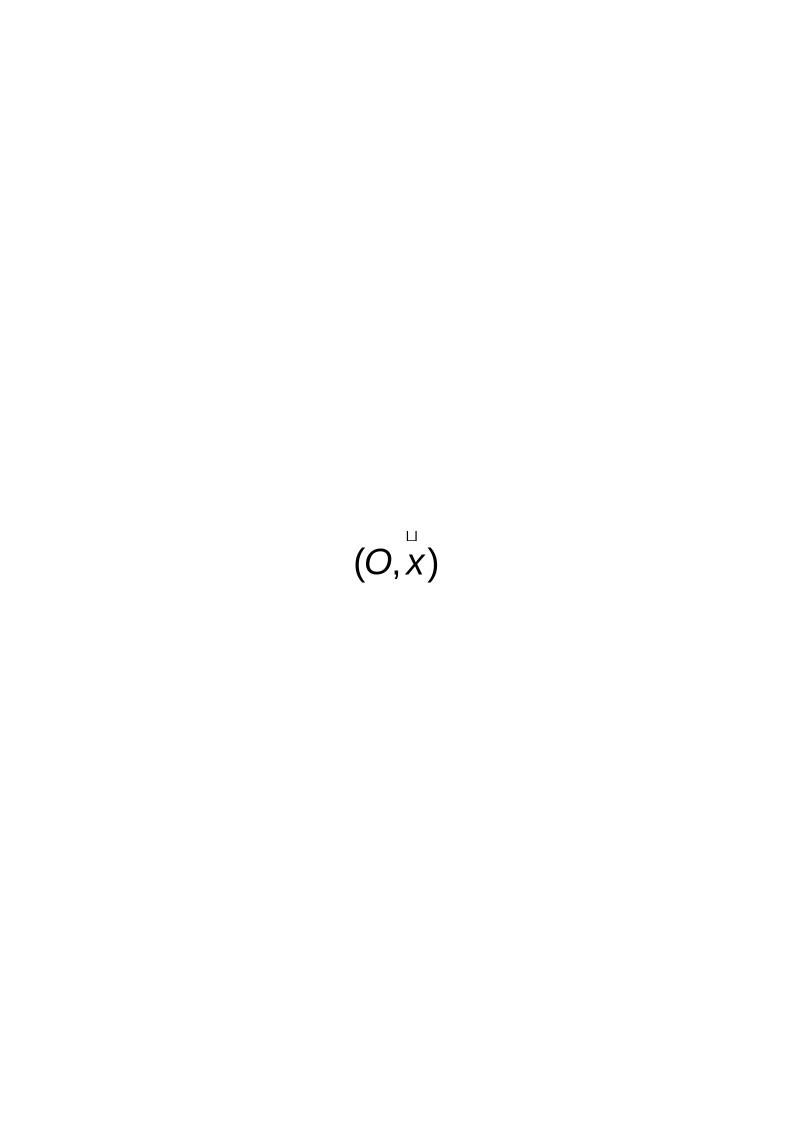
\includegraphics{images/image28.png}
\end{minipage} \\
& \begin{minipage}[b]{\linewidth}\raggedright
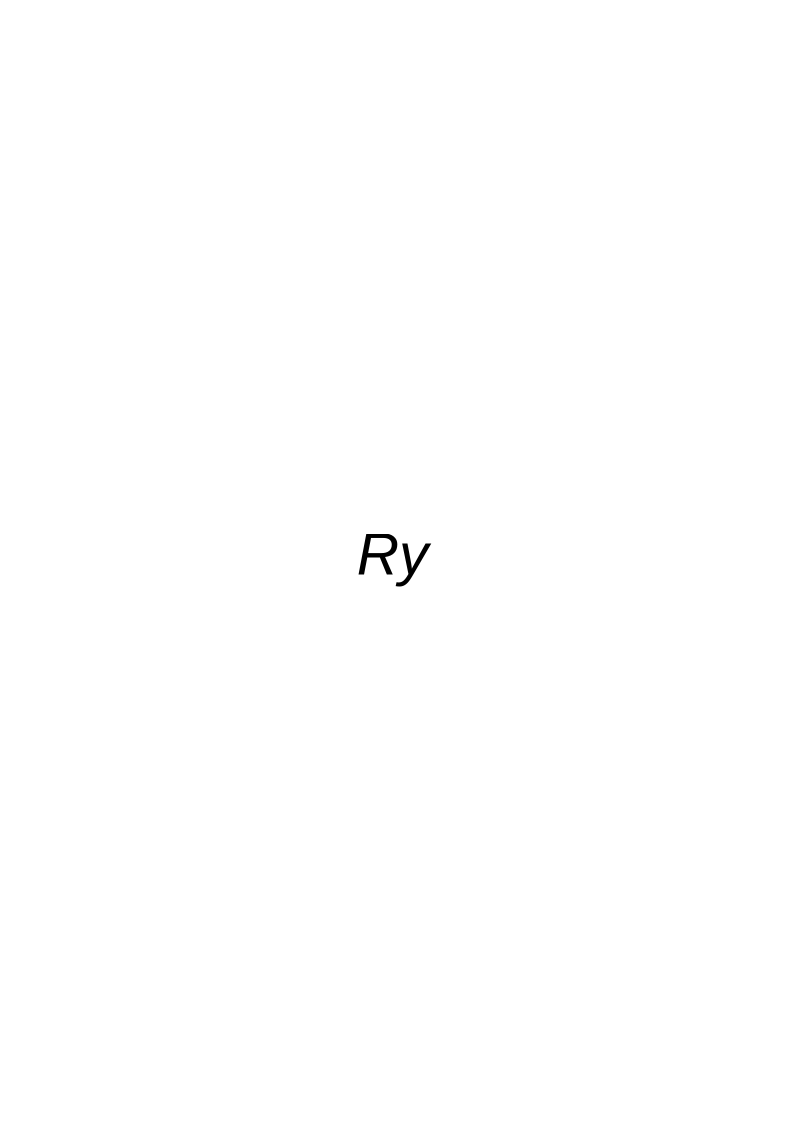
\includegraphics{images/image29.png} = liberté de mouvement de rotation
d'axe 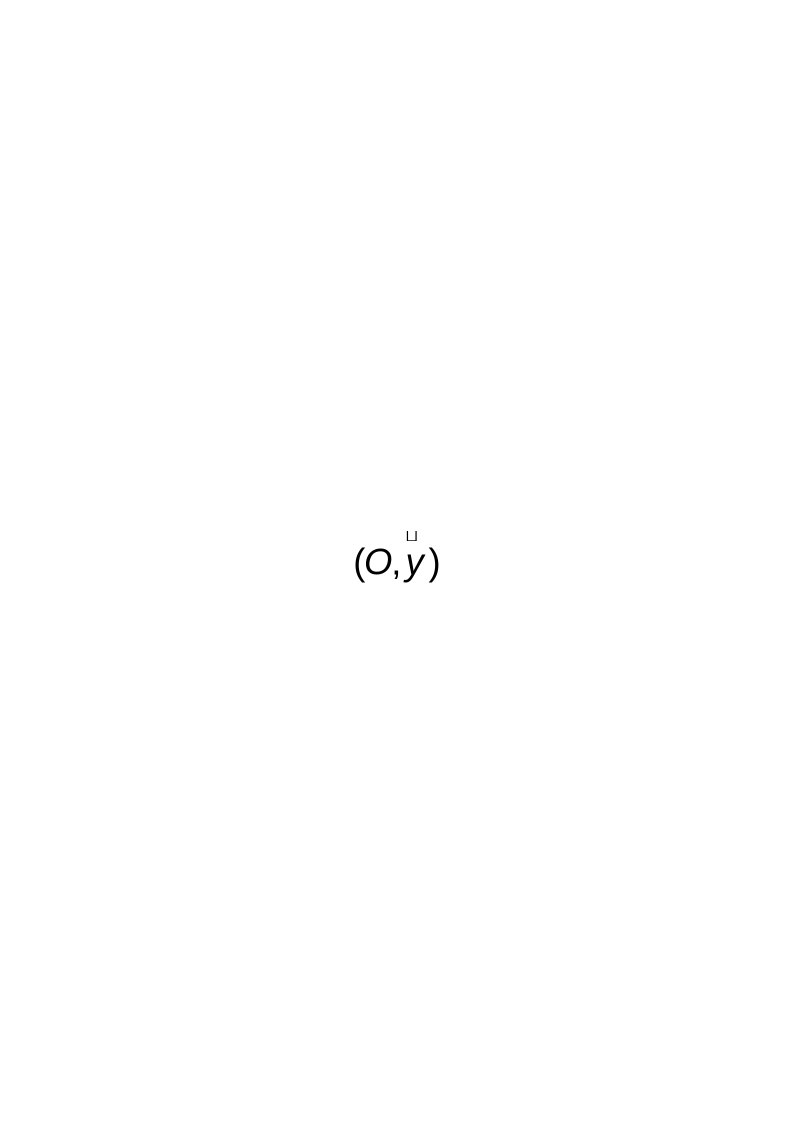
\includegraphics{images/image30.png}
\end{minipage} \\
& \begin{minipage}[b]{\linewidth}\raggedright
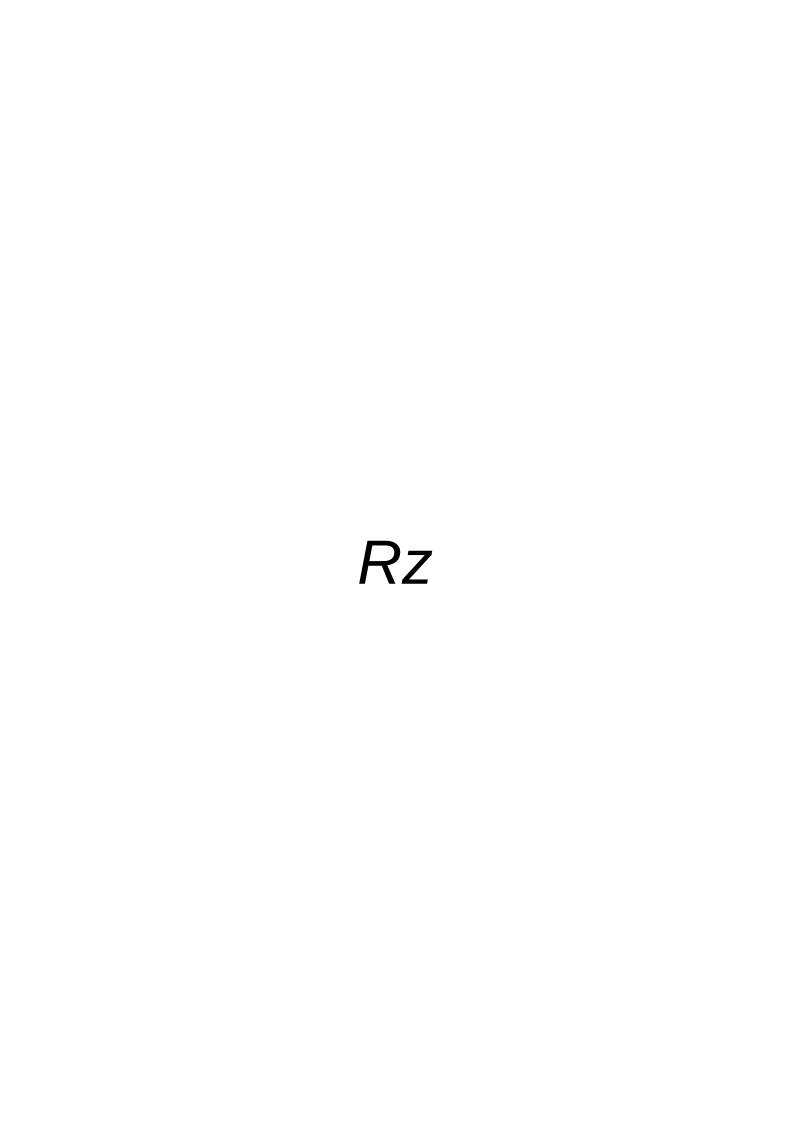
\includegraphics{images/image31.png} = liberté de mouvement de rotation
d'axe 
\includegraphics{images/image32.png}
\end{minipage} \\
\midrule\noalign{}
\endhead
\bottomrule\noalign{}
\endlastfoot
\end{longtable}

Le \emph{\textbf{nombre de degrés de liberté}} entre deux solides
correspond donc au \emph{\textbf{nombre de paramètres de mouvements
indépendants}} à définir pour caractériser le mouvement relatif entre
deux solides.

\subsection{\texorpdfstring{\hfill\break
Descriptions des
liaisons}{ Descriptions des liaisons}}\label{descriptions-des-liaisons}

Pour chacune des liaisons d'un mécanisme, on associe~:

\begin{longtable}[]{@{}
  >{\raggedright\arraybackslash}p{(\columnwidth - 2\tabcolsep) * \real{0.4784}}
  >{\raggedright\arraybackslash}p{(\columnwidth - 2\tabcolsep) * \real{0.5216}}@{}}
\toprule\noalign{}
\begin{minipage}[b]{\linewidth}\raggedright
\end{minipage} & \begin{minipage}[b]{\linewidth}\raggedright
REMARQUES
\end{minipage} \\
\midrule\noalign{}
\endhead
\bottomrule\noalign{}
\endlastfoot
Le nom & \multirow{2}{=}{\emph{Deux noms différents peuvent être
utilisés pour désigner la même liaison}

\emph{Deux liaisons différentes peuvent porter des noms qui se
ressemblent}} \\
\emph{\ul{Exemple~:}}

Liaison pivot \\
La description géométrique &
\multirow{2}{=}{\begin{minipage}[t]{\linewidth}\raggedright
\emph{Cette indication indispensable doit être rattachée au nom de la
liaison. Petit rappel~:}

\begin{itemize}
\item
  \emph{Cylindre -\textgreater{} axe}
\item
  \emph{Plan -\textgreater{} normale}
\end{itemize}
\end{minipage}} \\
\emph{\ul{Exemple~:}}

Liaison pivot d'axe 
\includegraphics{images/image33.png} \\
Les symboles de représentation 2D et 3D & \multirow{2}{=}{\emph{Ils ont
uniquement comme but de définir les mouvements relatifs possibles, sans
préjuger des solutions techniques présentent sur le système
réel\textbf{.}}

\emph{Les solides en contact seront donc indifféremment attachés à l'un
ou l'autre partie du symbole. Le choix se fera en fonction des critères
de lecture ou esthétique du schéma cinématique}} \\
\emph{\ul{Exemple~:}}


\includegraphics[width=\linewidth]{images/image34.png} \\
Le tableau de mobilité ou le nombre de degrés de liberté &
\multirow{2}{=}{\emph{Lorsque deux solides en mouvement relatifs sont en
contact, le nombre de degrés de liberté est compris entre 1 et 5.}} \\
\begin{minipage}[t]{\linewidth}\raggedright
\emph{\ul{Exemple~:}}

\begin{longtable}[]{@{}
  >{\raggedright\arraybackslash}p{(\columnwidth - 4\tabcolsep) * \real{0.5881}}
  >{\raggedright\arraybackslash}p{(\columnwidth - 4\tabcolsep) * \real{0.1775}}
  >{\raggedright\arraybackslash}p{(\columnwidth - 4\tabcolsep) * \real{0.2343}}@{}}
\toprule\noalign{}
\begin{minipage}[b]{\linewidth}\raggedright
\end{minipage} & \begin{minipage}[b]{\linewidth}\raggedright
\textbf{R}
\end{minipage} & \begin{minipage}[b]{\linewidth}\raggedright
\textbf{T}
\end{minipage} \\
\midrule\noalign{}
\endhead
\bottomrule\noalign{}
\endlastfoot
\(\overrightarrow{\mathbf{x}_{\mathbf{1}}}\) & 1 & 0 \\
\(\overrightarrow{\mathbf{y}_{\mathbf{1}}}\) & 0 & 0 \\
\(\overrightarrow{\mathbf{z}_{\mathbf{1}}}\) & 0 & 0 \\
\end{longtable}

1 degré de liberté~: Rotation suivant l'axe
\(\overrightarrow{\mathbf{x}_{\mathbf{1}}}\)
\end{minipage} \\
Le paramétrage associé aux degrés de liberté & \multirow{2}{=}{\emph{Il
sert à paramétrer la position (linéaire ou angulaire) relative d'un
solide par rapport à l'autre. Dans le cas des paramètres de rotation,
\textbf{il est fortement conseillé de le faire apparaître sur une figure
plane de changement de base}.}} \\
\emph{\ul{Exemple~:}}


\includegraphics[width=\linewidth]{images/image35.png} \\
Le torseur cinématique & \multirow{2}{=}{\emph{En général exprimé en un
point caractéristique de la liaison, il caractérise le comportement
cinématique d'un solide par rapport à l'autre.}

\emph{Il regroupe les informations permettant de déterminer le vecteur
vitesse de n'importe quel point d'un des deux solides dans son mouvement
par rapport à l'autre solide.}} \\
\emph{\ul{Exemple~:}}


\includegraphics{images/image36.png} \\
\end{longtable}

\subsection{Liaisons simples}\label{liaisons-simples}

Les liaisons simples sont celles obtenues par contact entre deux solides
élémentaires qui sont obtenues facilement en fabrication~:

\begin{itemize}
\item
  Le plan
\item
  Le cylindre (plein -- appelé aussi arbre-, ou creux -appelé aussi
  alésage)
\item
  La sphère (pleine ou creuse)
\end{itemize}

L`association de ces formes géométriques élémentaires amène à des
liaisons simples et contacts simples (surfacique, ponctuel, linéique) et
sont faciles à reconnaitre. De plus les caractéristiques géométriques
sont :

\begin{itemize}
\item
  Plan, il faut donner la normale au plan
\item
  Cylindre, il faut donner l'axe du cylindre
\item
  Sphère~: pas de spécificité
\end{itemize}

\begin{longtable}[]{@{}
  >{\raggedright\arraybackslash}p{(\columnwidth - 6\tabcolsep) * \real{0.1245}}
  >{\raggedright\arraybackslash}p{(\columnwidth - 6\tabcolsep) * \real{0.3287}}
  >{\raggedright\arraybackslash}p{(\columnwidth - 6\tabcolsep) * \real{0.2468}}
  >{\raggedright\arraybackslash}p{(\columnwidth - 6\tabcolsep) * \real{0.3000}}@{}}
\toprule\noalign{}
\begin{minipage}[b]{\linewidth}\raggedright
\end{minipage} & \begin{minipage}[b]{\linewidth}\raggedright
Plan
\end{minipage} & \begin{minipage}[b]{\linewidth}\raggedright
Sphère
\end{minipage} & \begin{minipage}[b]{\linewidth}\raggedright
Cylindre
\end{minipage} \\
\midrule\noalign{}
\endhead
\bottomrule\noalign{}
\endlastfoot
Plan &
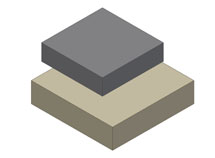
\includegraphics[width=\linewidth]{images/image37.jpeg}

Appui-plan de normale \ldots{}

\textbf{Contact surfacique} &
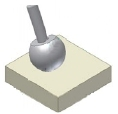
\includegraphics[width=\linewidth]{images/image38.jpeg}Sphère-plan
de normale \ldots{}

\textbf{Contact ponctuel} &
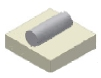
\includegraphics[width=\linewidth]{images/image39.jpeg}

Cylindre-plan de normale \ldots{} et d'axe\ldots{}

\textbf{Contact linéique} \\
Sphère &
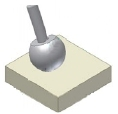
\includegraphics[width=\linewidth]{images/image38.jpeg}

Sphère-plan de normale \ldots{}

\textbf{Contact ponctuel} &
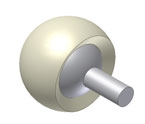
\includegraphics[width=\linewidth]{images/image40.jpeg}

Sphérique

\textbf{Contact surfacique} &
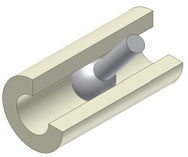
\includegraphics[width=\linewidth]{images/image41.jpeg}

Sphère-cylindre d'axe \ldots{}

\textbf{Contact linéique} \\
Cylindre &
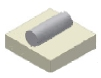
\includegraphics[width=\linewidth]{images/image39.jpeg}

Cylindre-plan de normale \ldots{} et d'axe\ldots{}

\textbf{Contact linéique} &
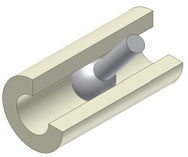
\includegraphics[width=\linewidth]{images/image41.jpeg}Sphère-cylindre
d'axe \ldots{}

\textbf{Contact linéique} &
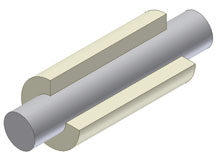
\includegraphics[width=\linewidth]{images/image42.jpeg}

Pivot glissant d'axe\ldots.

\textbf{Contact surfacique} \\
\end{longtable}

\begin{longtable}[]{@{}
  >{\raggedright\arraybackslash}p{(\columnwidth - 8\tabcolsep) * \real{0.2466}}
  >{\raggedright\arraybackslash}p{(\columnwidth - 8\tabcolsep) * \real{0.1708}}
  >{\raggedright\arraybackslash}p{(\columnwidth - 8\tabcolsep) * \real{0.1504}}
  >{\raggedright\arraybackslash}p{(\columnwidth - 8\tabcolsep) * \real{0.1606}}
  >{\raggedright\arraybackslash}p{(\columnwidth - 8\tabcolsep) * \real{0.2717}}@{}}
\toprule\noalign{}
\multirow{2}{=}{\begin{minipage}[b]{\linewidth}\raggedright
\textbf{Désignation de la liaison}

\textbf{Type de contact}
\end{minipage}} &
\multicolumn{2}{>{\raggedright\arraybackslash}p{(\columnwidth - 8\tabcolsep) * \real{0.3212} + 2\tabcolsep}}{%
\begin{minipage}[b]{\linewidth}\raggedright
\textbf{Symbole}
\end{minipage}} &
\multirow{2}{=}{\begin{minipage}[b]{\linewidth}\raggedright
\textbf{Mobilités}

\textbf{Degrés de liberté}
\end{minipage}} &
\multirow{2}{=}{\begin{minipage}[b]{\linewidth}\raggedright
\textbf{Torseur cinématique}\({\ \left\{ V_{2/1} \right\}}_{\text{O}}\)
\end{minipage}} \\
& \begin{minipage}[b]{\linewidth}\raggedright
\textbf{Plan}
\end{minipage} & \begin{minipage}[b]{\linewidth}\raggedright
\textbf{Spatial}
\end{minipage} \\
\midrule\noalign{}
\endhead
\bottomrule\noalign{}
\endlastfoot
Appui plan de normale \(\overrightarrow{\text{z}}\)


\includegraphics[width=\linewidth]{images/image43.emf}

\emph{Surfacique}

(plan / plan) &
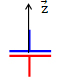
\includegraphics[width=\linewidth]{images/image44.jpeg}
&
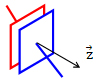
\includegraphics[width=\linewidth]{images/image45.jpeg}
& \(\ \begin{matrix}
0 \\
0 \\
\text{Rz}
\end{matrix}\ \left| \ \begin{matrix}
\text{Tx} \\
\text{Ty} \\
0
\end{matrix} \right.\ \)

\emph{3 paramètres indépendants}

\emph{= 3 ddl} &
\({{\ \left\{ V_{2/1} \right\}}_{\text{O}} =_{}^{}\left\{ \text{ }\begin{matrix}
\text{0} \\
\text{0} \\
\text{ω}_{\text{z 2/1}}
\end{matrix}\text{ }\left| \text{ }\begin{matrix}
\text{V}_{\text{x O, 2/1}} \\
\text{V}_{\text{y O, 2/1}} \\
\text{0}
\end{matrix} \right.\ \text{ } \right\}}_{\text{O,R}}\)

Pour tout point P de l\textquotesingle espace

Dans toute base contenant la normale (ici
\(\overrightarrow{\text{z}}\)) \\
Sphère-Plan (ou ponctuelle) de normale
\(\left( \text{O,}\overrightarrow{\text{z}} \right)\)


\includegraphics[width=\linewidth]{images/image46.emf}

\emph{Ponctuel} (sphère / plan) &
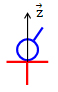
\includegraphics[width=\linewidth]{images/image47.jpeg}

O &
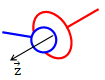
\includegraphics[width=\linewidth]{images/image48.jpeg}

O & \(\begin{matrix}
\text{Rx} \\
\text{Ry} \\
\text{Rz}
\end{matrix}\ \left| \ \begin{matrix}
\text{Tx} \\
\text{Ty} \\
\text{0}
\end{matrix} \right.\ \)

\emph{5 paramètres indépendants}

\emph{= 5 ddl} &
\({{\ \left\{ V_{2/1} \right\}}_{\text{O}} =_{}^{}\left\{ \text{ }\begin{matrix}
\text{ω}_{\text{x 2/1}} \\
\text{ω}_{\text{y 2/1}} \\
\text{ω}_{\text{z 2/1}}
\end{matrix}\text{ }\left| \text{ }\begin{matrix}
\text{V}_{\text{x O, 2/1}} \\
\text{V}_{\text{y O, 2/1}} \\
\text{0}
\end{matrix} \right.\ \text{ } \right\}}_{\text{O,R}}\)

Pour tout point P de l\textquotesingle axe
\(\left( \text{O,}\overrightarrow{\text{z}} \right)\)

Dans toute base contenant \(\overrightarrow{\text{z}}\) \\
Sphère-cylindre (ou linéaire annulaire) d'axe
\(\left( \text{O,}\overrightarrow{\text{z}} \right)\)


\includegraphics[width=\linewidth]{images/image49.emf}

\emph{Linéique}

(sphère / cylindre) &
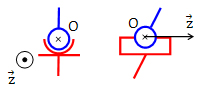
\includegraphics[width=\linewidth]{images/image50.jpeg}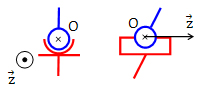
\includegraphics[width=\linewidth]{images/image50.jpeg}
&

\includegraphics[width=\linewidth]{images/image51.jpeg}
& \(\begin{matrix}
\text{Rx} \\
\text{Ry} \\
\text{Rz}
\end{matrix}\ \left| \ \begin{matrix}
0 \\
\text{0} \\
\text{Tz}
\end{matrix} \right.\ \)

\emph{4 paramètres indépendants}

\emph{= 4 ddl} &
\({{\ \left\{ V_{2/1} \right\}}_{\text{O}} =_{}^{}\left\{ \text{ }\begin{matrix}
\text{ω}_{\text{x 2/1}} \\
\text{ω}_{\text{y 2/1}} \\
\text{ω}_{\text{z 2/1}}
\end{matrix}\text{ }\left| \text{ }\begin{matrix}
\text{0} \\
0 \\
\text{V}_{\text{z O, 2/1}}
\end{matrix} \right.\ \text{ } \right\}}_{\text{O,R}}\)

Au centre O de la sphère

Dans toute base contenant \(\overrightarrow{\text{z}}\) \\
Cylindre-plan (ou linéaire rectiligne) d'axe
\(\left( \text{O,}\overrightarrow{\text{y}} \right)\) et de normale
\(\overrightarrow{\text{z}}\)
\includegraphics[width=\linewidth]{images/image52.emf}

\emph{Linéique} (plan / cylindre) &
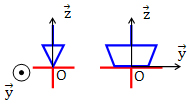
\includegraphics[width=\linewidth]{images/image53.jpeg}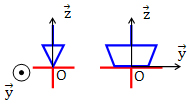
\includegraphics[width=\linewidth]{images/image53.jpeg}
&
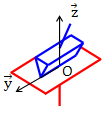
\includegraphics[width=\linewidth]{images/image54.jpeg}
& \(\begin{matrix}
0 \\
\text{Ry} \\
\text{Rz}
\end{matrix}\ \left| \ \begin{matrix}
\text{Tx} \\
\text{Ty} \\
0
\end{matrix} \right.\ \)

\emph{4 paramètres indépendants}

\emph{= 4 ddl} &
\({{\ \left\{ V_{2/1} \right\}}_{\text{O}} =_{}^{}\left\{ \text{ }\begin{matrix}
\text{0} \\
\text{ω}_{\text{y 2/1}} \\
\text{ω}_{\text{z 2/1}}
\end{matrix}\text{ }\left| \text{ }\begin{matrix}
\text{V}_{\text{x O, 2/1}}\  \\
\text{V}_{\text{y O, 2/1}} \\
\text{0}
\end{matrix} \right.\ \text{ } \right\}}_{\text{O,R}}\)

Pour tout point P du plan (yOz) \\
Sphérique (ou rotule) de centre O


\includegraphics[width=\linewidth]{images/image55.emf}

\emph{Surfacique}

(sphère / sphère) &
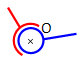
\includegraphics[width=\linewidth]{images/image56.jpeg}
&
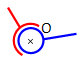
\includegraphics[width=\linewidth]{images/image56.jpeg}
& \(\begin{matrix}
\text{Rx} \\
\text{Ry} \\
\text{Rz}
\end{matrix}\ \left| \ \begin{matrix}
0 \\
\text{0} \\
0
\end{matrix}\ \  \right.\ \)

\emph{3 paramètres indépendants}

\emph{= 3 ddl} &
\({{\ \left\{ V_{2/1} \right\}}_{\text{O}} =_{}^{}\left\{ \text{ }\begin{matrix}
\text{ω}_{\text{x 2/1}} \\
\text{ω}_{\text{y 2/1}} \\
\text{ω}_{\text{z 2/1}}
\end{matrix}\text{ }\left| \text{ }\begin{matrix}
\text{0} \\
\text{0} \\
\text{0}
\end{matrix} \right.\ \text{ } \right\}}_{\text{O,R}}\)

Au centre O de la liaison

Dans toute base \\
Pivot glissant d'axe
\(\left( \text{O,}\overrightarrow{\text{z}} \right)\)


\includegraphics[width=\linewidth]{images/image57.emf}

\emph{Surfacique}

(cylindre / cylindre) &
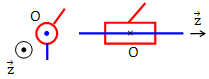
\includegraphics[width=\linewidth]{images/image58.jpeg}

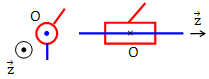
\includegraphics[width=\linewidth]{images/image58.jpeg}
&
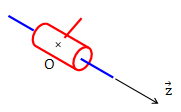
\includegraphics[width=\linewidth]{images/image59.jpeg}
& \(\begin{matrix}
\text{0} \\
\text{0} \\
\text{Rz}
\end{matrix}\ \left| \ \begin{matrix}
\text{0} \\
\text{0} \\
\text{Tz}
\end{matrix} \right.\ \)

\emph{2 paramètres indépendants}

\emph{= 2 ddl} &
\({{\ \left\{ V_{2/1} \right\}}_{\text{O}} =_{}^{}\left\{ \text{ }\begin{matrix}
\text{0} \\
\text{0} \\
\text{ω}_{\text{z 2/1}}
\end{matrix}\text{ }\left| \text{ }\begin{matrix}
\text{0} \\
0 \\
\text{V}_{\text{z O, 2/1}}
\end{matrix} \right.\ \text{ } \right\}}_{\text{O,R}}\)

Pour tout point P appartenant à
l\textquotesingle axe\(\left( \text{O,}\overrightarrow{\text{z}} \right)\)

Dans toute base contenant \(\overrightarrow{\text{z}}\) \\
\end{longtable}

\begin{longtable}[]{@{}
  >{\raggedright\arraybackslash}p{(\columnwidth - 2\tabcolsep) * \real{0.1227}}
  >{\raggedright\arraybackslash}p{(\columnwidth - 2\tabcolsep) * \real{0.8773}}@{}}
\toprule\noalign{}
\begin{minipage}[b]{\linewidth}\raggedright
\begin{quote}

\includegraphics[width=\linewidth]{images/image60.png}
\end{quote}
\end{minipage} & \begin{minipage}[b]{\linewidth}\raggedright
\begin{enumerate}
\def\labelenumi{\arabic{enumi}.}
\item
  Compléter le tableau suivant
\end{enumerate}

\begin{longtable}[]{@{}
  >{\raggedright\arraybackslash}p{(\columnwidth - 6\tabcolsep) * \real{0.2679}}
  >{\raggedright\arraybackslash}p{(\columnwidth - 6\tabcolsep) * \real{0.5459}}
  >{\raggedright\arraybackslash}p{(\columnwidth - 6\tabcolsep) * \real{0.0013}}
  >{\raggedright\arraybackslash}p{(\columnwidth - 6\tabcolsep) * \real{0.1849}}@{}}
\toprule\noalign{}
\multirow{2}{=}{\begin{minipage}[b]{\linewidth}\raggedright
\textbf{Désignation de la liaison}
\end{minipage}} &
\multicolumn{2}{>{\raggedright\arraybackslash}p{(\columnwidth - 6\tabcolsep) * \real{0.5472} + 2\tabcolsep}}{%
\begin{minipage}[b]{\linewidth}\raggedright
\textbf{Symbole}
\end{minipage}} & \begin{minipage}[b]{\linewidth}\raggedright
\textbf{Tableau de mobilités}
\end{minipage} \\
& \begin{minipage}[b]{\linewidth}\raggedright
\textbf{Plan}
\end{minipage} &
\multicolumn{2}{>{\raggedright\arraybackslash}p{(\columnwidth - 6\tabcolsep) * \real{0.1862} + 2\tabcolsep}@{}}{%
\begin{minipage}[b]{\linewidth}\raggedright
\end{minipage}} \\
\midrule\noalign{}
\endhead
\bottomrule\noalign{}
\endlastfoot
Pivot glissant axe (B,\(\overrightarrow{\text{z}}\)) & &
\multicolumn{2}{>{\raggedright\arraybackslash}p{(\columnwidth - 6\tabcolsep) * \real{0.1862} + 2\tabcolsep}@{}}{%
} \\
&
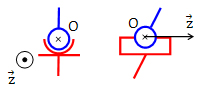
\includegraphics[width=\linewidth]{images/image50.jpeg}
&
\multicolumn{2}{>{\raggedright\arraybackslash}p{(\columnwidth - 6\tabcolsep) * \real{0.1862} + 2\tabcolsep}@{}}{%
} \\
& A

x &
\multicolumn{2}{>{\raggedright\arraybackslash}p{(\columnwidth - 6\tabcolsep) * \real{0.1862} + 2\tabcolsep}@{}}{%
R T

0 1

0 1

1 0} \\
Sphérique de centre T & &
\multicolumn{2}{>{\raggedright\arraybackslash}p{(\columnwidth - 6\tabcolsep) * \real{0.1862} + 2\tabcolsep}@{}}{%
} \\
&
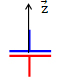
\includegraphics[width=\linewidth]{images/image44.jpeg}

Q &
\multicolumn{2}{>{\raggedright\arraybackslash}p{(\columnwidth - 6\tabcolsep) * \real{0.1862} + 2\tabcolsep}@{}}{%
} \\
sphère/plan de normale \((E,\overrightarrow{\text{z}}\)) & &
\multicolumn{2}{>{\raggedright\arraybackslash}p{(\columnwidth - 6\tabcolsep) * \real{0.1862} + 2\tabcolsep}@{}}{%
} \\
& B

x &
\multicolumn{2}{>{\raggedright\arraybackslash}p{(\columnwidth - 6\tabcolsep) * \real{0.1862} + 2\tabcolsep}@{}}{%
R T

0 1

1 0

1 1} \\
\end{longtable}
\end{minipage} \\
\midrule\noalign{}
\endhead
\bottomrule\noalign{}
\endlastfoot
\end{longtable}

Pour une liaison appui-plan, la seule rotation autorisée est celle de la
normale. Les translations et rotations sont complémentaires.

'\,'

Pour une liaison cylindre-plan, la seule translation impossible est
celle de la normale. La rotation impossible est suivant le seul axe non
indiqué dans la désignation.

'\,'

\subsection{Liaisons composées}\label{liaisons-composuxe9es}

Aux liaisons précédentes se rajoutent les liaisons composées, qui sont
(comme leur nom l'indique) composées de plusieurs liaisons élémentaires
précédentes (en parallèle ou en série)~:

\begin{itemize}
\item
  Liaison pivot d'axe\ldots.
\item
  Liaison glissière de direction\ldots.
\item
  Liaison sphérique à doigt de rotation interdite \ldots{}
\item
  Liaison hélicoïdale d'axe \ldots.
\end{itemize}

\begin{longtable}[]{@{}
  >{\raggedright\arraybackslash}p{(\columnwidth - 6\tabcolsep) * \real{0.2445}}
  >{\raggedright\arraybackslash}p{(\columnwidth - 6\tabcolsep) * \real{0.2445}}
  >{\raggedright\arraybackslash}p{(\columnwidth - 6\tabcolsep) * \real{0.2729}}
  >{\raggedright\arraybackslash}p{(\columnwidth - 6\tabcolsep) * \real{0.2382}}@{}}
\toprule\noalign{}
\begin{minipage}[b]{\linewidth}\raggedright
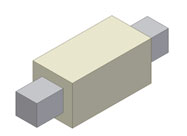
\includegraphics[width=\linewidth]{images/image61.jpeg}
\end{minipage} & \begin{minipage}[b]{\linewidth}\raggedright

\includegraphics[width=\linewidth]{images/image62.jpeg}
\end{minipage} & \begin{minipage}[b]{\linewidth}\raggedright
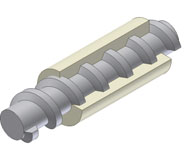
\includegraphics[width=\linewidth]{images/image63.jpeg}
\end{minipage} & \begin{minipage}[b]{\linewidth}\raggedright
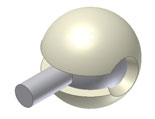
\includegraphics[width=\linewidth]{images/image64.jpeg}
\end{minipage} \\
\midrule\noalign{}
\endhead
\bottomrule\noalign{}
\endlastfoot
\textbf{GLISSIERE} & \textbf{PIVOT} & \textbf{HELICOIDALE} &
\textbf{SPHERIQUE A DOIGT} \\
\end{longtable}

Par exemple voici une liaison glissière de direction
\(\overrightarrow{j_{0}}\) composée de deux liaisons pivot glissant en
parallèle.

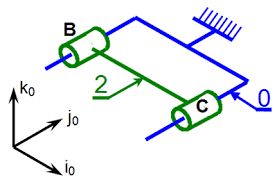
\includegraphics[width=\linewidth]{images/image65.png}

\begin{longtable}[]{@{}
  >{\raggedright\arraybackslash}p{(\columnwidth - 8\tabcolsep) * \real{0.2210}}
  >{\raggedright\arraybackslash}p{(\columnwidth - 8\tabcolsep) * \real{0.1954}}
  >{\raggedright\arraybackslash}p{(\columnwidth - 8\tabcolsep) * \real{0.1563}}
  >{\raggedright\arraybackslash}p{(\columnwidth - 8\tabcolsep) * \real{0.1694}}
  >{\raggedright\arraybackslash}p{(\columnwidth - 8\tabcolsep) * \real{0.2579}}@{}}
\toprule\noalign{}
\multirow{2}{=}{\begin{minipage}[b]{\linewidth}\raggedright
\textbf{Désignation de la liaison}
\end{minipage}} &
\multicolumn{2}{>{\raggedright\arraybackslash}p{(\columnwidth - 8\tabcolsep) * \real{0.3517} + 2\tabcolsep}}{%
\begin{minipage}[b]{\linewidth}\raggedright
\textbf{Symbole}
\end{minipage}} &
\multirow{2}{=}{\begin{minipage}[b]{\linewidth}\raggedright
\textbf{Mobilités}

\textbf{Degrés de liberté}
\end{minipage}} &
\multirow{2}{=}{\begin{minipage}[b]{\linewidth}\raggedright
\textbf{Torseur cinématique}\({\ \left\{ V_{2/1} \right\}}_{\text{O}}\)
\end{minipage}} \\
& \begin{minipage}[b]{\linewidth}\raggedright
\textbf{Plan}
\end{minipage} & \begin{minipage}[b]{\linewidth}\raggedright
\textbf{Spatial}
\end{minipage} \\
\midrule\noalign{}
\endhead
\bottomrule\noalign{}
\endlastfoot
Glissière de direction \(\overrightarrow{\text{z}}\)


\includegraphics[width=\linewidth]{images/image66.emf}
&
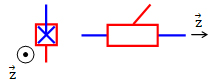
\includegraphics[width=\linewidth]{images/image67.jpeg}

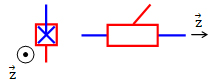
\includegraphics[width=\linewidth]{images/image67.jpeg}
&

\includegraphics[width=\linewidth]{images/image68.jpeg}
& \(\begin{matrix}
\text{0} \\
\text{0} \\
\text{0}
\end{matrix}\ \left| \ \begin{matrix}
\text{0} \\
\text{0} \\
\text{Tz}
\end{matrix} \right.\ \)

\emph{1 paramètre indépendant}

\emph{= 1 ddl} &
\({{\ \left\{ V_{2/1} \right\}}_{\text{O}} =_{}^{}\left\{ \text{ }\begin{matrix}
\text{0} \\
\text{0} \\
\text{0}
\end{matrix}\text{ }\left| \text{ }\begin{matrix}
\text{0} \\
0 \\
\text{V}_{\text{z O, }\text{2/1}}
\end{matrix} \right.\ \text{ } \right\}}_{\text{O,}\text{R}}\)

Pour tout point P de l\textquotesingle espace

Dans toute base contenant \(\overrightarrow{\text{z}}\) \\
Pivot d'axe \(\left( \text{O,}\overrightarrow{\text{z}} \right)\)


\includegraphics[width=\linewidth]{images/image69.emf}
& 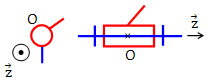
\includegraphics[width=\linewidth]{images/image70.jpeg}

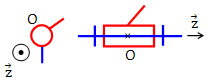
\includegraphics[width=\linewidth]{images/image70.jpeg}
&
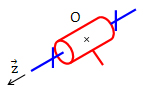
\includegraphics[width=\linewidth]{images/image71.jpeg}
& \(\begin{matrix}
\text{0} \\
\text{0} \\
\text{Rz}
\end{matrix}\ \left| \ \begin{matrix}
\text{0} \\
\text{0} \\
0
\end{matrix} \right.\ \)

\emph{1 paramètre indépendant}

\emph{= 1 ddl} &
\({{\ \left\{ V_{2/1} \right\}}_{\text{O}} =_{}^{}\left\{ \text{ }\begin{matrix}
\text{0} \\
\text{0} \\
\text{ω}_{\text{z 2/1}}
\end{matrix}\text{ }\left| \text{ }\begin{matrix}
\text{0} \\
0 \\
\text{0}
\end{matrix} \right.\ \text{ } \right\}}_{\text{O,R}}\)

Pour tout point P appartenant à
l\textquotesingle axe\(\left( \text{O,}\overrightarrow{\text{z}} \right)\)

-Dans toute base contenant \(\overrightarrow{\text{z}}\) \\
Hélicoïdale d'axe \(\left( \text{O,}\overrightarrow{\text{z}} \right)\)


\includegraphics[width=\linewidth]{images/image72.emf} &

\includegraphics[width=\linewidth]{images/image73.jpeg}


\includegraphics[width=\linewidth]{images/image73.jpeg}
&

\includegraphics[width=\linewidth]{images/image74.jpeg}
& \(\begin{matrix}
\text{0} \\
\text{0} \\
\text{Rz}
\end{matrix}\ \left| \ \begin{matrix}
\text{0} \\
\text{0} \\
\text{Tz}
\end{matrix} \right.\ \)

Rz et Tz liées

\emph{\textbf{1 paramètre indépendant}}

\emph{\textbf{= 1 ddl}} &
\({{\ \left\{ V_{2/1} \right\}}_{\text{O}} =_{}^{}\left\{ \text{ }\begin{matrix}
\text{0} \\
\text{0} \\
\text{ω}_{\text{z 2/1}}
\end{matrix}\text{ }\left| \text{ }\begin{matrix}
\text{0} \\
0 \\
\text{V}_{\text{z O, 2/1}}
\end{matrix} \right.\ \text{ } \right\}}_{\text{O,R}}\)

\(\text{V}_{\text{z O, 2/1}}\) et \(\text{ω}_{\text{z 2/1}}\ \)liées :
\(\text{V}_{\text{z O, }\text{2/1}} =\)p.\(\ \frac{\text{ω}_{\text{z 2/1}}}{2\pi}\)

Pour tout point P appartenant à
l\textquotesingle axe\(\left( \text{O,}\overrightarrow{\text{z}} \right)\)

Dans toute base contenant \(\overrightarrow{\text{z}}\) \\
Sphérique à doigt de centre O et de rotation interdite
\(\left( \text{O,}\overrightarrow{\text{z}} \right)\)


\includegraphics[width=\linewidth]{images/image75.emf}
&
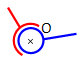
\includegraphics[width=\linewidth]{images/image56.jpeg}
&
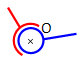
\includegraphics[width=\linewidth]{images/image56.jpeg}
& \(\begin{matrix}
\text{Rx} \\
\text{Ry} \\
\text{0}
\end{matrix}\ \left| \ \begin{matrix}
0 \\
\text{0} \\
0
\end{matrix}\ \  \right.\ \)

\emph{2 paramètres indépendants}

\emph{= 2 ddl} &
\({{\ \left\{ V_{2/1} \right\}}_{\text{O}} =_{}^{}\left\{ \text{ }\begin{matrix}
\text{ω}_{\text{x }\text{2/1}} \\
\text{ω}_{\text{y }\text{2/1}} \\
\text{0}
\end{matrix}\text{ }\left| \text{ }\begin{matrix}
\text{0} \\
\text{0} \\
\text{0}
\end{matrix} \right.\ \text{ } \right\}}_{\text{O,}\text{R}}\)

Au centre O de la liaison \\
\end{longtable}

\begin{longtable}[]{@{}
  >{\raggedright\arraybackslash}p{(\columnwidth - 2\tabcolsep) * \real{0.1227}}
  >{\raggedright\arraybackslash}p{(\columnwidth - 2\tabcolsep) * \real{0.8773}}@{}}
\toprule\noalign{}
\begin{minipage}[b]{\linewidth}\raggedright
\begin{quote}

\includegraphics[width=\linewidth]{images/image60.png}
\end{quote}
\end{minipage} & \begin{minipage}[b]{\linewidth}\raggedright
Un vérin électrique peut se modéliser par le schéma cinématique suivant
:

O

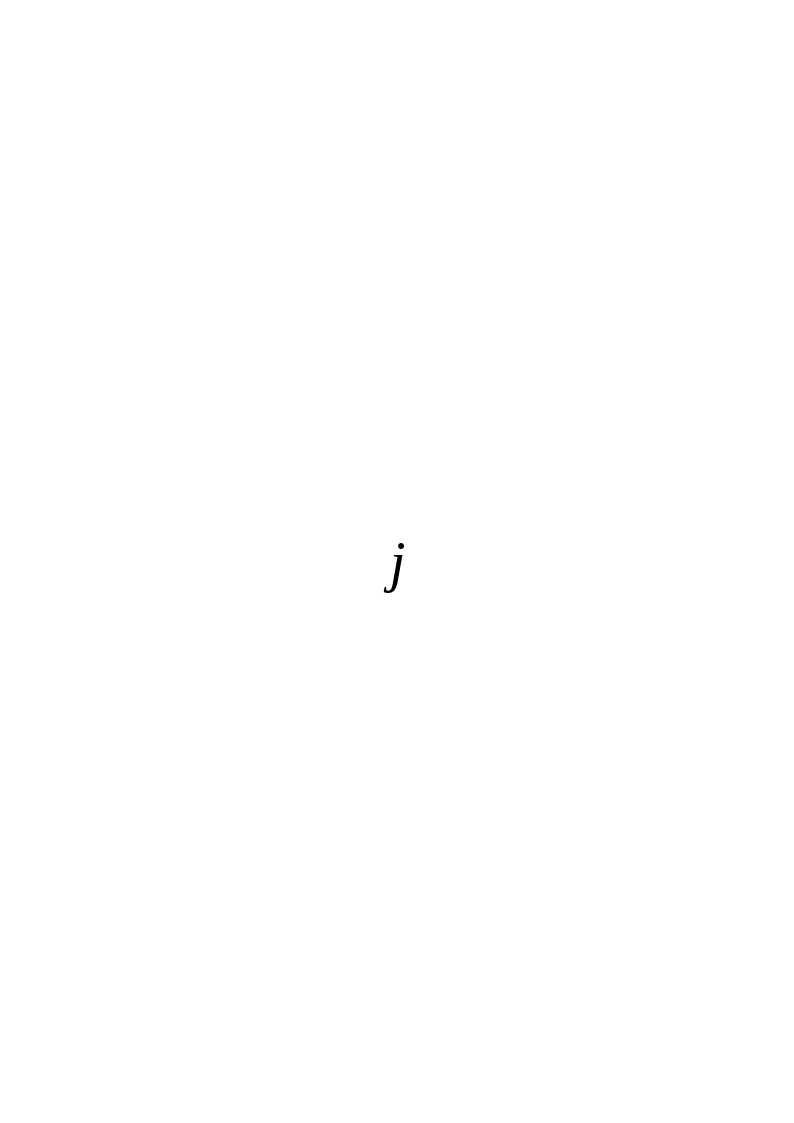
\includegraphics{images/image76.png}

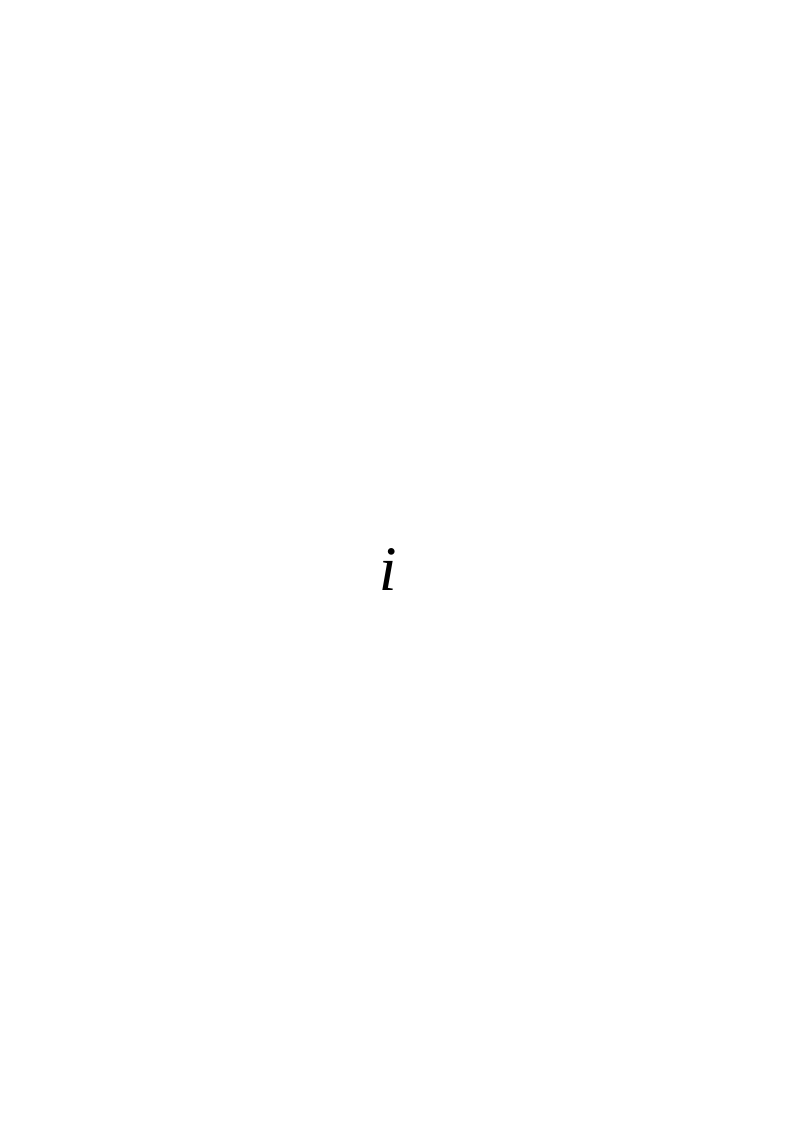
\includegraphics{images/image77.png}


\includegraphics[width=\linewidth]{images/image78.jpeg}
\includegraphics[width=\linewidth]{images/image79.jpeg}

C

A

\begin{enumerate}
\def\labelenumi{\arabic{enumi}.}
\setcounter{enumi}{1}
\item
  Donner le graphe de liaisons correspondant
\item
  Donner les torseurs cinématiques \(\left\{ V_{2/1} \right\}_{B}\),
  \(\left\{ V_{2/0} \right\}_{A}\)et
  \(\left\{ V_{1/0} \right\}_{O}\)associés aux trois liaisons du schéma
  cinématique.
\end{enumerate}
\end{minipage} \\
\midrule\noalign{}
\endhead
\bottomrule\noalign{}
\endlastfoot
\end{longtable}

\section{ELABORATION D'UN MODELE
CINEMATIQUE}\label{elaboration-dun-modele-cinematique}

\subsection{Démarche}\label{duxe9marche}

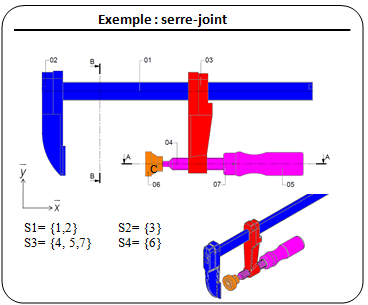
\includegraphics[width=\linewidth]{images/image80.png}\textbf{Etape
1 : Identifier les Classes d'Equivalence Cinématique} (Solides
Cinématiquement liés)

Cela consiste à repérer sur le système réel les pièces qui n'ont pas de
mouvement relatif entre elles et à les regrouper. Pour cela :

\begin{itemize}
\item
  rechercher et/ou colorier chaque CEC sur la représentation technique
  2D ou 3D du système;
\item
  nommer chacune des CEC (S1, S2\ldots) et lister, dans l'ordre
  croissant, les pièces qui les constituent.
\end{itemize}

\begin{itemize}
\item
  \textbf{Remarque~:} Toutes les pièces déformables CEC (ressorts,
  rondelles élastiques, barres de torsion, joints\ldots) et les éléments
  roulants (billes, rouleaux\ldots) des roulements, butées, douilles,
  vis et guidages sont à exclure des CEC.
\end{itemize}

\begin{quote}

\includegraphics[width=\linewidth]{images/image81.png}
\includegraphics[width=\linewidth]{images/image82.png}
\includegraphics[width=\linewidth]{images/image83.png}
\end{quote}


\includegraphics[width=\linewidth]{images/image84.png}\textbf{Etape
2 : Réaliser le graphe des liaisons}

Pour cela :

\begin{itemize}
\item
  représenter les CEC par des bulles et les placer en respectant si
  possible leurs positions relatives observées sur le système réel;
\item
  repérer la CEC qui correspond au solide considéré comme fixe ;
\item
  identifier les mouvements relatifs entre deux CEC en contact, choisir
  la liaison usuelle associée et la représenter par un lien entre les
  deux bulles.
\end{itemize}

Pour trouver les liaisons, on peut utiliser les deux questions
suivantes~:

\begin{itemize}
\item
  \emph{\textbf{Quelle est la nature des surfaces en contact entre les
  solides~? (contact ponctuel, linéique ou surfacique)}}
\item
  \emph{\textbf{Quels sont les mouvements relatifs possibles entre les
  solides~? (translations et rotations).}}
\end{itemize}

\textbf{Remarque~:} Lorsque cela est possible, on peut simplifier le
graphe des liaisons en remplaçant des liaisons en parallèles ou en série
par leur liaison équivalente (voir un peu plus tard~:D).

Cela permet d'obtenir un \emph{\textbf{graphe des liaisons minimal}} qui
peut être plus adapté à l'étude que l'on souhaite ensuite réaliser.

\textbf{Etape 3 : Elaborer le schéma cinématique}


\includegraphics[width=\linewidth]{images/image3.png}Pour
cela :

\begin{itemize}
\item
  positionner les centres et les axes des liaisons en respectant si
  possible leurs positions relatives observées sur le système réel;
\item
  mettre en place, en s'appuyant sur le graphe des liaisons, les
  symboles des liaisons usuelles en utilisant le code couleur retenu et
  en respectant leur orientation;
\item
  relier par des traits les éléments des symboles de liaisons qui sont
  de même couleur en respectant si possible l'architecture du système
  réel et en évitant que des traits se croisent.
\item
  vérifier la cohérence entre les mouvements possibles entre les CEC sur
  le schéma cinématique et les mouvements observés sur le système réel.
\end{itemize}

\textbf{Remarque~:} si le schéma cinématique a été conçu en s'appuyant
sur le graphe des liaisons minimal, on parle du \emph{\textbf{\ul{schéma
cinématique minimal}.}}

\begin{longtable}[]{@{}
  >{\raggedright\arraybackslash}p{(\columnwidth - 2\tabcolsep) * \real{0.1227}}
  >{\raggedright\arraybackslash}p{(\columnwidth - 2\tabcolsep) * \real{0.8773}}@{}}
\toprule\noalign{}
\begin{minipage}[b]{\linewidth}\raggedright
\begin{quote}

\includegraphics[width=\linewidth]{images/image60.png}
\end{quote}
\end{minipage} & \begin{minipage}[b]{\linewidth}\raggedright
Réaliser le graphe de liaison et le schéma cinématique du micromoteur.


\includegraphics[width=\linewidth]{images/image85.gif}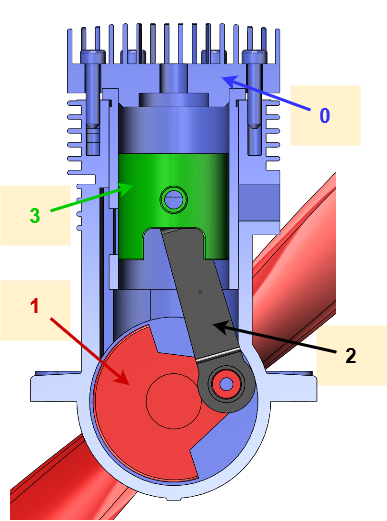
\includegraphics[width=\linewidth]{images/image86.png}

\textbf{Etape 1~: Identifier les classes d'équivalences}

\textbf{Ici, il est assez simple d'identifier 4 solides~:}

\begin{itemize}
\item
  \textbf{0~: le carter}
\item
  \textbf{1~: le vilebrequin}
\item
  \textbf{2~: la bielle}
\item
  \textbf{3~: le piston}
\end{itemize}

\textbf{Le solide de référence, appelé aussi bâti, doit être unique}.
C'est le solide «~fixe~» dans le référentiel d'observation (par
hypothèse Galiléen). On lui attribue une base, en général
\((\overrightarrow{x_{0}},\overrightarrow{y_{0}},\overrightarrow{z_{0}})\).
Ici le bâti est le carter \textbf{\ul{0}}.

\textbf{Etape 2~: Graphe de liaison}

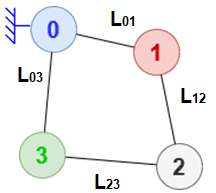
\includegraphics{images/image87.png}Il existe différentes approches
permettant d'identifier par quelle liaison cinématique normalisée
modéliser un contact entre deux solides :

\begin{itemize}
\item
  analyse approfondie couples de \textbf{surfaces en contact}
  (plan/plan, sphère/cylindre, \ldots)
\item
  analyse des \textbf{degrés de liberté} autorisés par la liaison
  \textbf{(sans tenir compte du reste du mécanisme !)}
\item
  identification de composants dont la fonction est le guidage en
  rotation ou en translation (roulements à billes, \ldots)
\item
  
\includegraphics[width=\linewidth]{images/image88.gif}ou
  une combinaison de ces méthodes \ldots{}
\end{itemize}

On en déduit la nature de la liaison entre le piston et le carte :
\textbf{pivot glissant} d'axe (\emph{A},
\(\overrightarrow{z_{0}}\)\emph{)}

~Chaque liaison doit être \ul{complètement décrite} (nom et éléments de
situation) ; on définit les différents points nécessaires pour cela.


\includegraphics[width=\linewidth]{images/image89.png}Exemple
: pour le micromoteur, on a besoin des 3 points \emph{A}, \emph{B} et
\emph{C}.

Et l'on peut ainsi définir toutes les liaisons du mécanisme :

\begin{itemize}
\item
  L\textsubscript{01} : \textbf{pivot} d'axe (\emph{A},
  \(\overrightarrow{z_{0}})\)
\item
  L\textsubscript{12} : \textbf{pivot} d'axe (\emph{B},
  \(\overrightarrow{z_{0}})\).
\item
  L\textsubscript{23} : \textbf{pivot glissant} d'axe (\emph{C},
  \(\overrightarrow{z_{0}})\).
\item
  L\textsubscript{30} : \textbf{pivot glissant} d'axe (\emph{A},
  \(\overrightarrow{y_{0}})\).
\end{itemize}

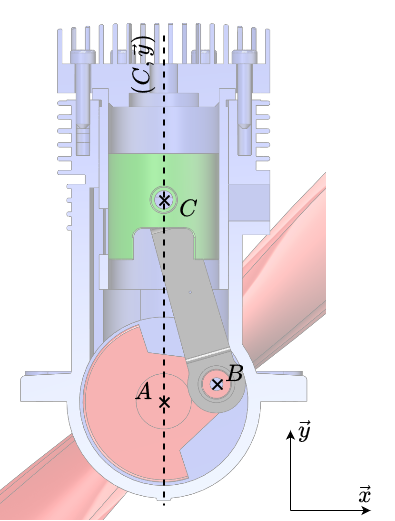
\includegraphics[width=\linewidth]{images/image90.png}~\textbf{Etape
3~: Elaborer le schéma cinématique}

On choisit une vue adaptée. Dans le cas du micromoteur, le plan
\((\overrightarrow{x_{0}},\overrightarrow{y_{0}}\)) convient bien. On
met en place les éléments de situation des liaisons (axes,
points,\ldots)

Remarque : seule la \ul{position relative} des points est nécessaire.
Inutile de respecter absolument les dimensions.

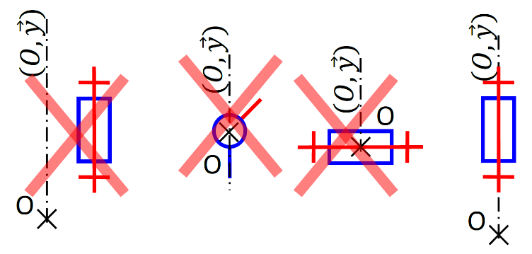
\includegraphics[width=\linewidth]{images/image91.png}~On
dessine les symboles normalisés des liaisons, positionnés et orientés
selon les éléments de situation de chacun. Attention à ne pas commettre
d'erreur de positionnement~!

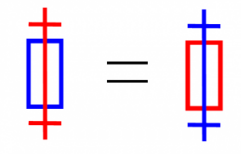
\includegraphics[width=\linewidth]{images/image92.png}Remarque
: le choix de la couleur n'a pas d'influence sur le modèle cinématique.

Exemple : 4 symboles de liaisons pour le micromoteur, représentés \ul{en
respectant les couleurs des solides} !

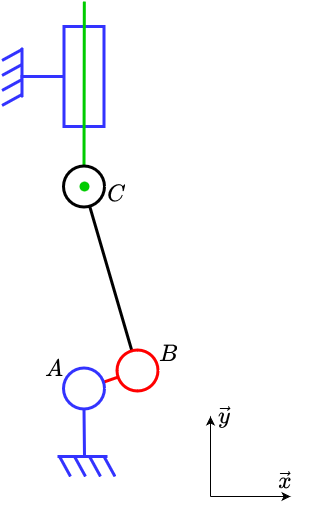
\includegraphics[width=\linewidth]{images/image93.png}~

On représentera le « bâti » par ce symbole :
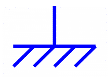
\includegraphics[width=\linewidth]{images/image94.png}

Exemple : voici un schéma cinématique du micromoteur
\end{minipage} \\
\midrule\noalign{}
\endhead
\bottomrule\noalign{}
\endlastfoot
& \\
\end{longtable}

\subsection{\texorpdfstring{Modélisation des guidages
}{Modélisation des guidages }}\label{moduxe9lisation-des-guidages}

Grâce à l'interposition d'\emph{\textbf{éléments glissants}} ou
\emph{\textbf{roulants}} entre les solides, il est possible d'obtenir
des mouvements relatifs plus performants d'un point de vue énergétique.
L'utilisation de ces solutions techniques permet aussi aux concepteurs
des systèmes d'obtenir facilement les mouvements relatifs recherchés.

\begin{longtable}[]{@{}
  >{\raggedright\arraybackslash}p{(\columnwidth - 6\tabcolsep) * \real{0.4746}}
  >{\raggedright\arraybackslash}p{(\columnwidth - 6\tabcolsep) * \real{0.0143}}
  >{\raggedright\arraybackslash}p{(\columnwidth - 6\tabcolsep) * \real{0.3281}}
  >{\raggedright\arraybackslash}p{(\columnwidth - 6\tabcolsep) * \real{0.1830}}@{}}
\toprule\noalign{}
\multicolumn{4}{@{}>{\raggedright\arraybackslash}p{(\columnwidth - 6\tabcolsep) * \real{1.0000} + 6\tabcolsep}@{}}{%
\begin{minipage}[b]{\linewidth}\raggedright
\textbf{Coussinets}
\end{minipage}} \\
\midrule\noalign{}
\endhead
\bottomrule\noalign{}
\endlastfoot

\includegraphics[width=\linewidth]{images/image95.png}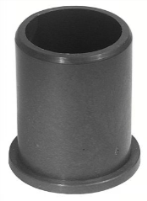
\includegraphics[width=\linewidth]{images/image96.png}
&
\multicolumn{3}{>{\raggedright\arraybackslash}p{(\columnwidth - 6\tabcolsep) * \real{0.5254} + 4\tabcolsep}@{}}{%
Ils permettent d'obtenir un mouvement relatif entre deux solides
modélisables par une liaison \textbf{pivot} ou \textbf{pivot
glissant}} \\
\multicolumn{4}{@{}>{\raggedright\arraybackslash}p{(\columnwidth - 6\tabcolsep) * \real{1.0000} + 6\tabcolsep}@{}}{%
} \\
\multicolumn{4}{@{}>{\raggedright\arraybackslash}p{(\columnwidth - 6\tabcolsep) * \real{1.0000} + 6\tabcolsep}@{}}{%
\textbf{Roulements}} \\
\multicolumn{3}{@{}>{\raggedright\arraybackslash}p{(\columnwidth - 6\tabcolsep) * \real{0.8170} + 4\tabcolsep}}{%

\includegraphics[width=\linewidth]{images/image97.png}En
fonction de la valeur de l'angle maximal \textbf{de rotulage} fourni par
le constructeur, on peut considérer que le mouvement relatif entre la
bague extérieure et la bague intérieure peut être modélisé par une
liaison pivot ou une liaison sphérique. \textbf{I}l existe toujours un
jeu, aussi minime soit-il, entre les billes et les bagues. Ce jeu a pour
conséquence de permettre une rotation relative des bagues, autour des
axes perpendiculaires à l\textquotesingle axe principal du roulement.

Si \textbf{l'angle maximal de rotulage est \textgreater5'}, on peut
considérer que les degrés de liberté de rotation autour des axes
secondaires ne sont pas supprimés.} &

\includegraphics[width=\linewidth]{images/image98.png} \\
\multicolumn{2}{@{}>{\raggedright\arraybackslash}p{(\columnwidth - 6\tabcolsep) * \real{0.4889} + 2\tabcolsep}}{%
Roulement à une rangée de billes

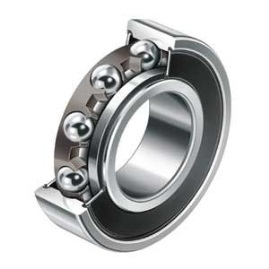
\includegraphics[width=\linewidth]{images/image99.jpeg}
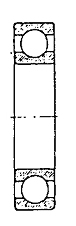
\includegraphics[width=\linewidth]{images/image100.jpeg}

En général, rotulage \textgreater{} 5'⇒ liaison \textbf{sphérique}} &
\multicolumn{2}{>{\raggedright\arraybackslash}p{(\columnwidth - 6\tabcolsep) * \real{0.5111} + 2\tabcolsep}@{}}{%
Roulement à deux rangées de billes

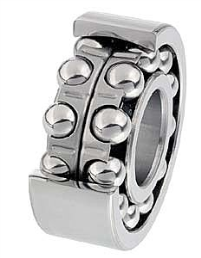
\includegraphics[width=\linewidth]{images/image101.png}
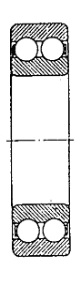
\includegraphics[width=\linewidth]{images/image102.jpeg}

En général, rotulage \textless{} 5'⇒ liaison \textbf{pivot}} \\
\multicolumn{2}{@{}>{\raggedright\arraybackslash}p{(\columnwidth - 6\tabcolsep) * \real{0.4889} + 2\tabcolsep}}{%
Roulement à aiguilles ou à rouleaux

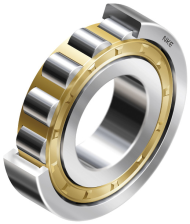
\includegraphics[width=\linewidth]{images/image103.png}
\includegraphics[width=\linewidth]{images/image104.png}
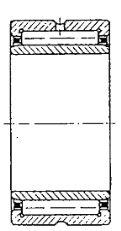
\includegraphics[width=\linewidth]{images/image105.jpeg}

Rotulage toujours \textless{} 5'⇒ liaison \textbf{pivot}} &
\multicolumn{2}{>{\raggedright\arraybackslash}p{(\columnwidth - 6\tabcolsep) * \real{0.5111} + 2\tabcolsep}@{}}{%
Roulement à rotule (billes ou rouleaux)


\includegraphics[width=\linewidth]{images/image106.jpeg}

\includegraphics[width=\linewidth]{images/image107.jpeg}

Rotulage entre 2°et 4°⇒ liaison \textbf{sphérique}} \\
\end{longtable}

Ainsi, la façon dont sont liées les bagues aux deux solides en contact
par l'intermédiaire du roulement, peut conduire à modéliser le mouvement
relatif d'un solide par rapport à l'autre par~:

\begin{longtable}[]{@{}
  >{\raggedright\arraybackslash}p{(\columnwidth - 6\tabcolsep) * \real{0.3377}}
  >{\raggedright\arraybackslash}p{(\columnwidth - 6\tabcolsep) * \real{0.1586}}
  >{\raggedright\arraybackslash}p{(\columnwidth - 6\tabcolsep) * \real{0.4957}}
  >{\raggedright\arraybackslash}p{(\columnwidth - 6\tabcolsep) * \real{0.0080}}@{}}
\toprule\noalign{}
\begin{minipage}[b]{\linewidth}\raggedright
\textbf{Une liaison pivot}
\end{minipage} &
\multicolumn{3}{>{\raggedright\arraybackslash}p{(\columnwidth - 6\tabcolsep) * \real{0.6623} + 4\tabcolsep}@{}}{%
\begin{minipage}[b]{\linewidth}\raggedright
\begin{itemize}
\item
  Angle de rotulage du roulement \textless5'
\item
  Les deux bagues sont ~arrêtées~ en translation
\end{itemize}
\end{minipage}} \\
\midrule\noalign{}
\endhead
\bottomrule\noalign{}
\endlastfoot
\textbf{Une liaison pivot glissant} &
\multicolumn{3}{>{\raggedright\arraybackslash}p{(\columnwidth - 6\tabcolsep) * \real{0.6623} + 4\tabcolsep}@{}}{%
\begin{minipage}[t]{\linewidth}\raggedright
\begin{itemize}
\item
  Angle de rotulage du roulement \textless5'
\item
  Une des deux bagues n'est pas arrêtée en translation
\end{itemize}
\end{minipage}} \\
\textbf{Une liaison sphérique} &
\multicolumn{3}{>{\raggedright\arraybackslash}p{(\columnwidth - 6\tabcolsep) * \real{0.6623} + 4\tabcolsep}@{}}{%
\begin{minipage}[t]{\linewidth}\raggedright
\begin{itemize}
\item
  Angle de rotulage du roulement \textgreater5'
\item
  Les deux bagues sont arrêtées~ en translation
\end{itemize}
\end{minipage}} \\
\textbf{Une liaison sphère-cylindre (ou linéaire annulaire)} &
\multicolumn{3}{>{\raggedright\arraybackslash}p{(\columnwidth - 6\tabcolsep) * \real{0.6623} + 4\tabcolsep}@{}}{%
\begin{minipage}[t]{\linewidth}\raggedright
\begin{itemize}
\item
  Angle de rotulage du roulement \textgreater5'
\item
  Une des deux bagues n'est pas arrêtée en translation
\end{itemize}
\end{minipage}} \\
\multicolumn{3}{@{}>{\raggedright\arraybackslash}p{(\columnwidth - 6\tabcolsep) * \real{0.9920} + 4\tabcolsep}}{%
\textbf{Douilles à billes}} & \\
\multicolumn{2}{@{}>{\raggedright\arraybackslash}p{(\columnwidth - 6\tabcolsep) * \real{0.4963} + 2\tabcolsep}}{%

\includegraphics[width=\linewidth]{images/image108.png}}
& Elles permettent d'obtenir un mouvement relatif entre deux solides
modélisable par une liaison \textbf{pivot glissant} & \\
\end{longtable}

\begin{longtable}[]{@{}
  >{\raggedright\arraybackslash}p{(\columnwidth - 2\tabcolsep) * \real{0.5003}}
  >{\raggedright\arraybackslash}p{(\columnwidth - 2\tabcolsep) * \real{0.4997}}@{}}
\toprule\noalign{}
\multicolumn{2}{@{}>{\raggedright\arraybackslash}p{(\columnwidth - 2\tabcolsep) * \real{1.0000} + 2\tabcolsep}@{}}{%
\begin{minipage}[b]{\linewidth}\raggedright
\textbf{Vis à billes}
\end{minipage}} \\
\midrule\noalign{}
\endhead
\bottomrule\noalign{}
\endlastfoot

\includegraphics[width=\linewidth]{images/image109.png}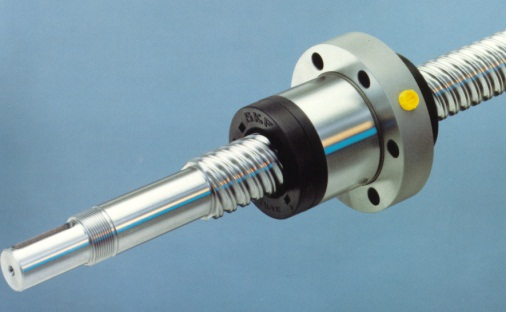
\includegraphics[width=\linewidth]{images/image110.jpeg}
& Elles permettent d'obtenir un mouvement relatif entre deux solides
modélisable par une liaison \textbf{hélicoïdale} \\
\end{longtable}

\begin{longtable}[]{@{}
  >{\raggedright\arraybackslash}p{(\columnwidth - 2\tabcolsep) * \real{0.5003}}
  >{\raggedright\arraybackslash}p{(\columnwidth - 2\tabcolsep) * \real{0.4997}}@{}}
\toprule\noalign{}
\multicolumn{2}{@{}>{\raggedright\arraybackslash}p{(\columnwidth - 2\tabcolsep) * \real{1.0000} + 2\tabcolsep}@{}}{%
\begin{minipage}[b]{\linewidth}\raggedright
\textbf{Guidages à billes}
\end{minipage}} \\
\midrule\noalign{}
\endhead
\bottomrule\noalign{}
\endlastfoot
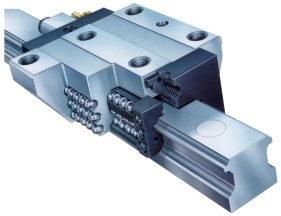
\includegraphics[width=\linewidth]{images/image111.jpeg}
& Ils permettent d'obtenir un mouvement relatif entre deux solides
modélisable par une liaison \textbf{glissière} \\
\multicolumn{2}{@{}>{\raggedright\arraybackslash}p{(\columnwidth - 2\tabcolsep) * \real{1.0000} + 2\tabcolsep}@{}}{%
\textbf{Rotules lisses}} \\

\includegraphics[width=\linewidth]{images/image112.png}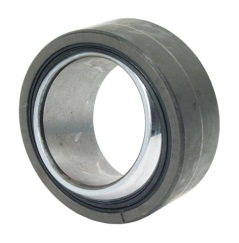
\includegraphics[width=\linewidth]{images/image113.jpeg}
& Elles permettent d'obtenir un mouvement relatif entre deux solides
modélisable par une liaison \textbf{sphérique} \\
\end{longtable}

\subsection{Modélisations des transmetteurs
usuels}\label{moduxe9lisations-des-transmetteurs-usuels}

On trouve, sur les systèmes réels, de nombreux dispositifs permettant
d'\emph{\textbf{adapter}} et de \emph{\textbf{transmettre l'énergie
mécanique}}. Il faut donc savoir représenter ou identifier dans un
schéma cinématique les plus courants d'entre eux.

\begin{longtable}[]{@{}
  >{\raggedright\arraybackslash}p{(\columnwidth - 2\tabcolsep) * \real{0.3444}}
  >{\raggedright\arraybackslash}p{(\columnwidth - 2\tabcolsep) * \real{0.6556}}@{}}
\toprule\noalign{}
\begin{minipage}[b]{\linewidth}\raggedright
Roue et vis sans fin
\end{minipage} &
\multirow{2}{=}{\begin{minipage}[b]{\linewidth}\raggedright

\includegraphics[width=\linewidth]{images/image114.png}
\end{minipage}} \\
\begin{minipage}[b]{\linewidth}\raggedright
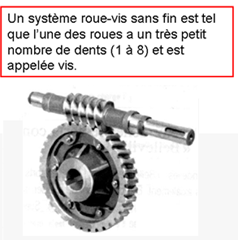
\includegraphics[width=\linewidth]{images/image115.png}
\end{minipage} \\
\midrule\noalign{}
\endhead
\bottomrule\noalign{}
\endlastfoot
Poulie-courroie &
\multirow{2}{=}{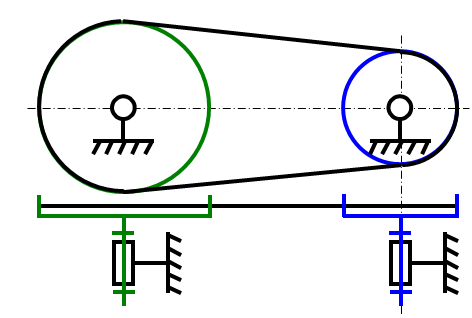
\includegraphics[width=\linewidth]{images/image116.png}} \\
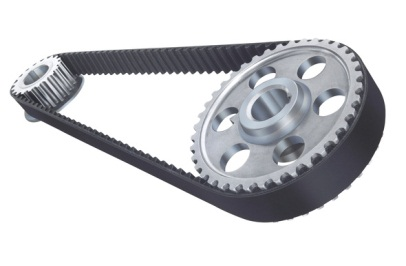
\includegraphics[width=\linewidth]{images/image117.jpeg} \\
Engrenages &
\multirow{2}{=}{
\includegraphics[width=\linewidth]{images/image118.png}} \\

\includegraphics[width=\linewidth]{images/image119.png} \\
\end{longtable}

\section{PARAMETRAGE D'UN SCHEMA
CINEMATIQUE}\label{parametrage-dun-schema-cinematique}

Afin de pouvoir simuler le comportement du mécanisme à l'aide des outils
(lois, principes fondamentaux) de la mécanique, on va associer une
\textbf{base} \textbf{orthonormée directe} à chaque classe
d'équivalence. Comme pour le solide de référence, on associe à chaque
solide dont on étudie le mouvement, un repère appelé repère associé au
solide. Au solide 1 sera associé le
repère\(\ (O_{1},\overrightarrow{x_{1}},\overrightarrow{y_{1}},\overrightarrow{z_{1}})\)
, au solide 2 le repère
\((O_{2},\overrightarrow{x_{2}},\overrightarrow{y_{2}},\overrightarrow{z_{2}})\)
\emph{\textsubscript{,}} etc\ldots{}

\begin{longtable}[]{@{}
  >{\raggedright\arraybackslash}p{(\columnwidth - 2\tabcolsep) * \real{0.1227}}
  >{\raggedright\arraybackslash}p{(\columnwidth - 2\tabcolsep) * \real{0.8773}}@{}}
\toprule\noalign{}
\begin{minipage}[b]{\linewidth}\raggedright
\begin{quote}

\includegraphics[width=\linewidth]{images/image60.png}
\end{quote}
\end{minipage} & \begin{minipage}[b]{\linewidth}\raggedright
\begin{enumerate}
\def\labelenumi{\arabic{enumi}.}
\item
  Paramétrer les schémas cinématiques.
\end{enumerate}


\includegraphics[width=\linewidth]{images/image120.png}\textbf{Antenne
parabolique}

\textbf{A}

\textbf{B}

\textbf{C}

\textbf{1}

\textbf{0}

\textbf{2}

\textbf{3}

\textbf{Echelle EPAS}


\includegraphics[width=\linewidth]{images/image121.png}

O\textsubscript{0}

A

C

B
\end{minipage} \\
\midrule\noalign{}
\endhead
\bottomrule\noalign{}
\endlastfoot
\end{longtable}

\subsection[Base
orthonormée]{\texorpdfstring{\protect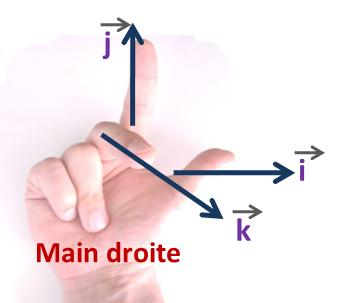
\includegraphics[width=\linewidth]{images/image124.jpeg}Base
orthonormée}{Base orthonormée}}\label{base-orthonormuxe9e}

En SII, les bases associées aux solides sont toujours des bases
orthonormées de dimension 3 avec les propriétés suivantes, elle sera :

\textbf{■ Orthonormée : - vecteurs orthogonaux 2 à 2}

\textbf{- de longueur unitaire (norme=1)}

■ \textbf{Directe}

Ces bases bougent avec les classes d'équivalences et sont donc en
mouvement les unes par rapport aux autres. Pour quantifier ces
mouvements on va utiliser des \textbf{paramètres de mouvement}.

Heureusement, les mouvements entres les solides d'un mécanisme sont très
simples en général~:

\begin{itemize}
\item
  La \textbf{translation rectiligne} (liaison glissière)
\item
  La \textbf{rotation autour d'un axe} (liaison \textbf{pivot})
\end{itemize}

Dans une \textbf{liaison pivot}, le mouvement relatif entre les deux
solides est un mouvement de \textbf{rotation}.

On veut donc savoir, à \textbf{chaque instant t}, de quel \textbf{angle}
a tourné la base associée au premier solide par rapport à la base
associée au deuxième solide. On va \textbf{paramétrer} cette liaison
avec un \textbf{angle (\emph{α,β,θ},\ldots) fonction du temps. Il y aura
donc une figure de changement de base.}

Dans une liaison \textbf{glissière}, le mouvement relatif entre les deux
solides est un mouvement de \textbf{translation rectiligne.} Le
paramètre de cette liaison est une \textbf{distance}. \textbf{Les bases
sont colinéaires et il n'y aura pas de figure de changement de base
entre les deux.}

\subsection{Figures de changement de
base}\label{figures-de-changement-de-base}

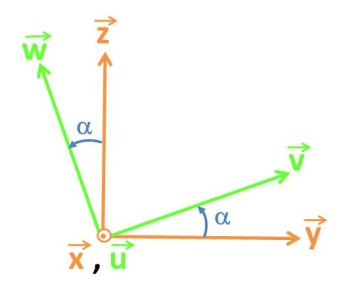
\includegraphics[width=\linewidth]{images/image125.jpeg}Pour
construire la \textbf{figure de changement de base}, il faut :

\begin{itemize}
\item
  \textbf{Dessiner} la figure de changement de base avec un
  \textbf{petit angle} (≈20°).
\item
  \textbf{Placer face à soi} le vecteur autour duquel tourne la base par
  rapport à l'autre. \emph{\textbf{(il s'agit donc d'un vecteur
  commun)}}
\item
  \textbf{Compléter de manière directe} les bases.
\end{itemize}

\begin{quote}
Il faut dessiner autant de figures de changement de base qu'il y a de
liaisons pivot dans le mécanisme étudié. Dans ce cas, certaines règles
sont à respecter afin de faciliter les calculs qui seront réalisés à
partir de ces figures (produits vectoriels et produits scalaires). Il
faut :
\end{quote}

\begin{itemize}
\item
  toujours superposer les figures lorsque cela est possible,
  c'est-à-dire lorsque plusieurs figures ont un même vecteur unitaire
  commun, ce qui est le cas lorsqu'il y a plusieurs liaisons pivot
  d'axes parallèles.
\item
  reporter sur toutes les figures les égalités de vecteur unitaire.
\end{itemize}

\begin{longtable}[]{@{}
  >{\raggedright\arraybackslash}p{(\columnwidth - 2\tabcolsep) * \real{0.1227}}
  >{\raggedright\arraybackslash}p{(\columnwidth - 2\tabcolsep) * \real{0.8773}}@{}}
\toprule\noalign{}
\begin{minipage}[b]{\linewidth}\raggedright
\begin{quote}

\includegraphics[width=\linewidth]{images/image60.png}
\end{quote}
\end{minipage} & \begin{minipage}[b]{\linewidth}\raggedright
\begin{enumerate}
\def\labelenumi{\arabic{enumi}.}
\item
  Réaliser les figures de changement de base de l'antenne parabolique et
  de l'échelle EPAS
\end{enumerate}

\textbf{Antenne parabolique}

\textbf{Echelle EPAS}
\end{minipage} \\
\midrule\noalign{}
\endhead
\bottomrule\noalign{}
\endlastfoot
\end{longtable}

\begin{longtable}[]{@{}
  >{\raggedright\arraybackslash}p{(\columnwidth - 2\tabcolsep) * \real{0.1227}}
  >{\raggedright\arraybackslash}p{(\columnwidth - 2\tabcolsep) * \real{0.8773}}@{}}
\toprule\noalign{}
\begin{minipage}[b]{\linewidth}\raggedright
\begin{quote}

\includegraphics[width=\linewidth]{images/image60.png}
\end{quote}
\end{minipage} & \begin{minipage}[b]{\linewidth}\raggedright
🢩 Soit une base
\(({\overrightarrow{x}}_{1},{\overrightarrow{y}}_{1},{\overrightarrow{z}}_{1})\)
en rotation par rapport à la base
\(({\overrightarrow{x}}_{0},{\overrightarrow{y}}_{0},{\overrightarrow{z}}_{0})\)

\textbf{α} est le paramètre qui caractérise la rotation autour de l'axe
\({\overrightarrow{z}}_{0}( = {\overrightarrow{z}}_{1})\) \textbf{→ α =}
\(({\overrightarrow{x}}_{0},{\overrightarrow{x}}_{1})\)

🢩 Soit une base
\(({\overrightarrow{x}}_{2},{\overrightarrow{y}}_{2},{\overrightarrow{z}}_{2})\)
en rotation par rapport à la base
\(({\overrightarrow{x}}_{1},{\overrightarrow{y}}_{1},{\overrightarrow{z}}_{1})\)

\textbf{β} est le paramètre qui caractérise la rotation autour de l'axe
\({\overrightarrow{x}}_{1}( = {\overrightarrow{x}}_{2})\) \textbf{→ β =}
\(({\overrightarrow{y}}_{1},{\overrightarrow{y}}_{2})\)

\textbf{1 - Dessiner} les figures de changement de base
\end{minipage} \\
\midrule\noalign{}
\endhead
\bottomrule\noalign{}
\endlastfoot
\end{longtable}

\begin{longtable}[]{@{}
  >{\raggedright\arraybackslash}p{(\columnwidth - 2\tabcolsep) * \real{0.1227}}
  >{\raggedright\arraybackslash}p{(\columnwidth - 2\tabcolsep) * \real{0.8773}}@{}}
\toprule\noalign{}
\begin{minipage}[b]{\linewidth}\raggedright
\begin{quote}

\includegraphics[width=\linewidth]{images/image60.png}
\end{quote}
\end{minipage} & \begin{minipage}[b]{\linewidth}\raggedright
\textbf{Robot de soudage}

On associe à chaque solide i une base orthonormée directe

\includegraphics{images/image126.png}

Le mouvement de 1/0 est une rotation d'axe
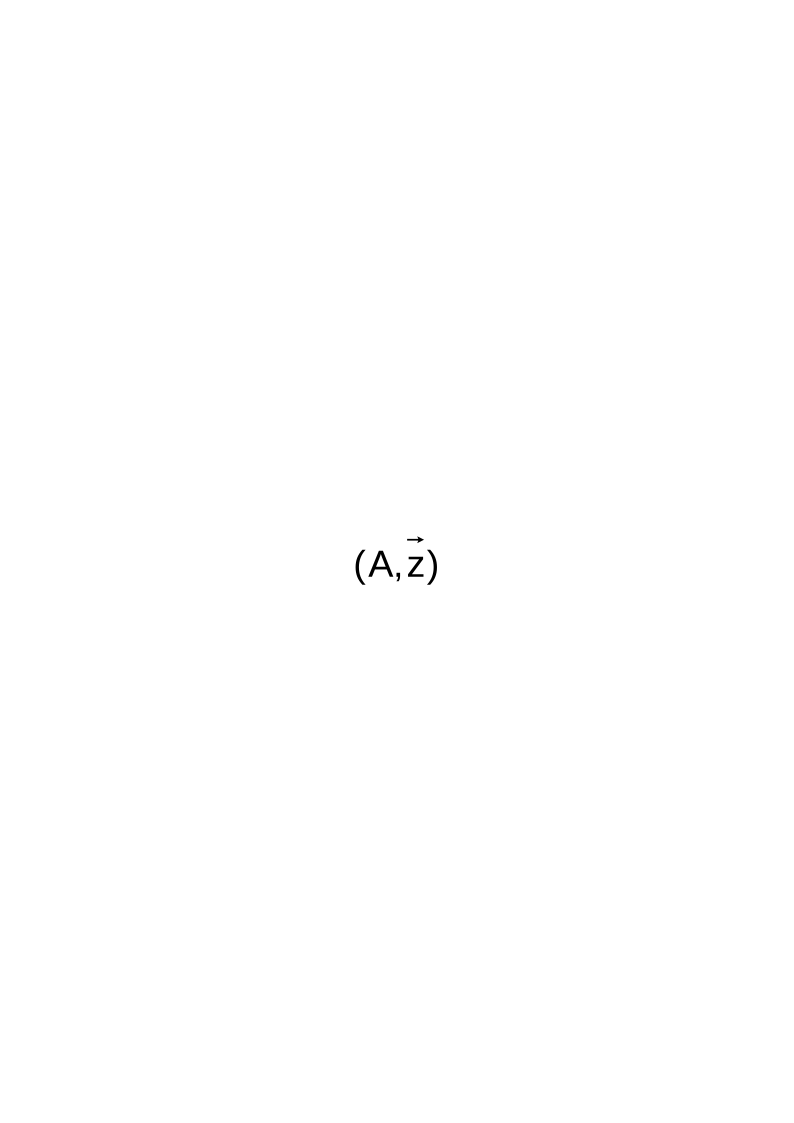
\includegraphics{images/image127.png}~; on pose
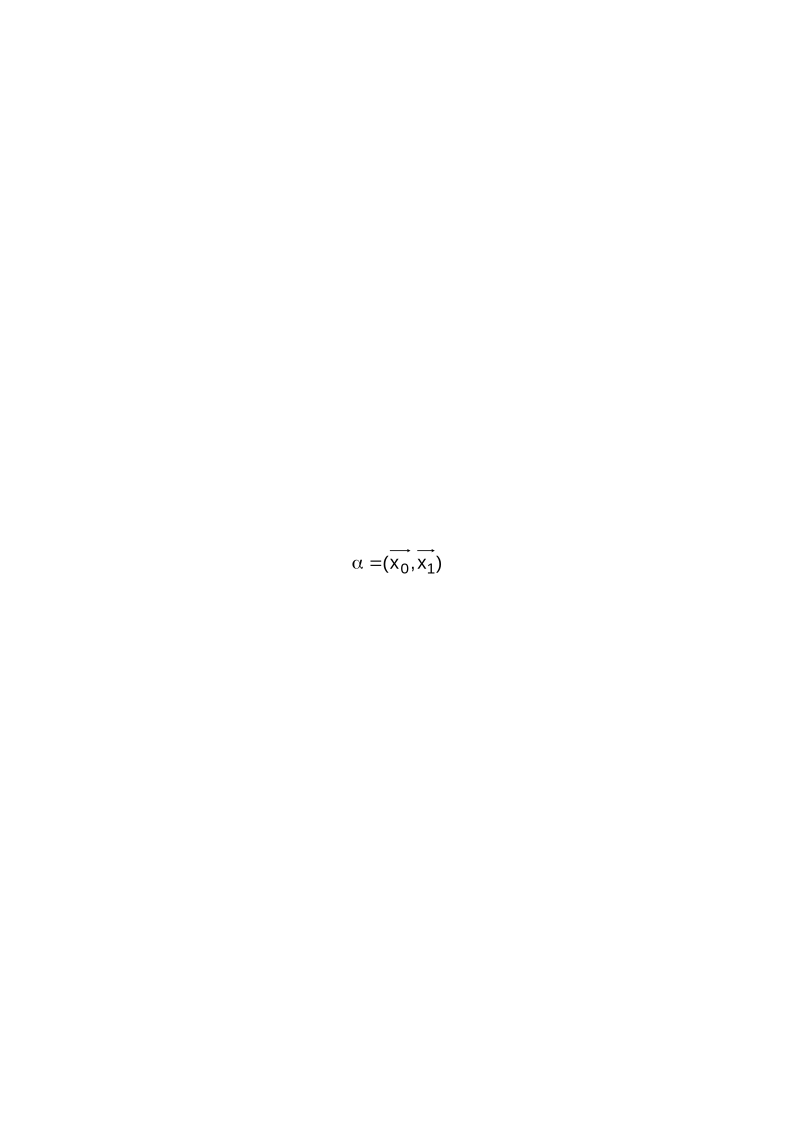
\includegraphics{images/image128.png}

Le mouvement de 2/0 est une rotation d'axe
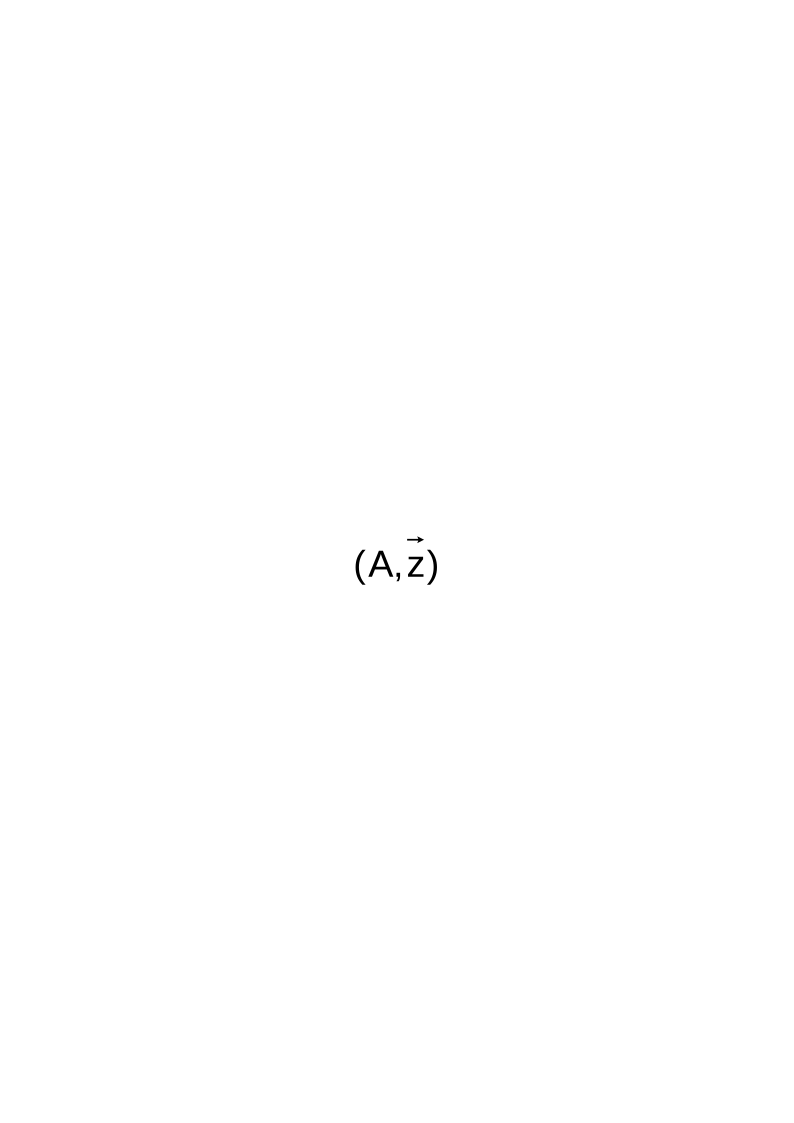
\includegraphics{images/image129.png}~; on pose
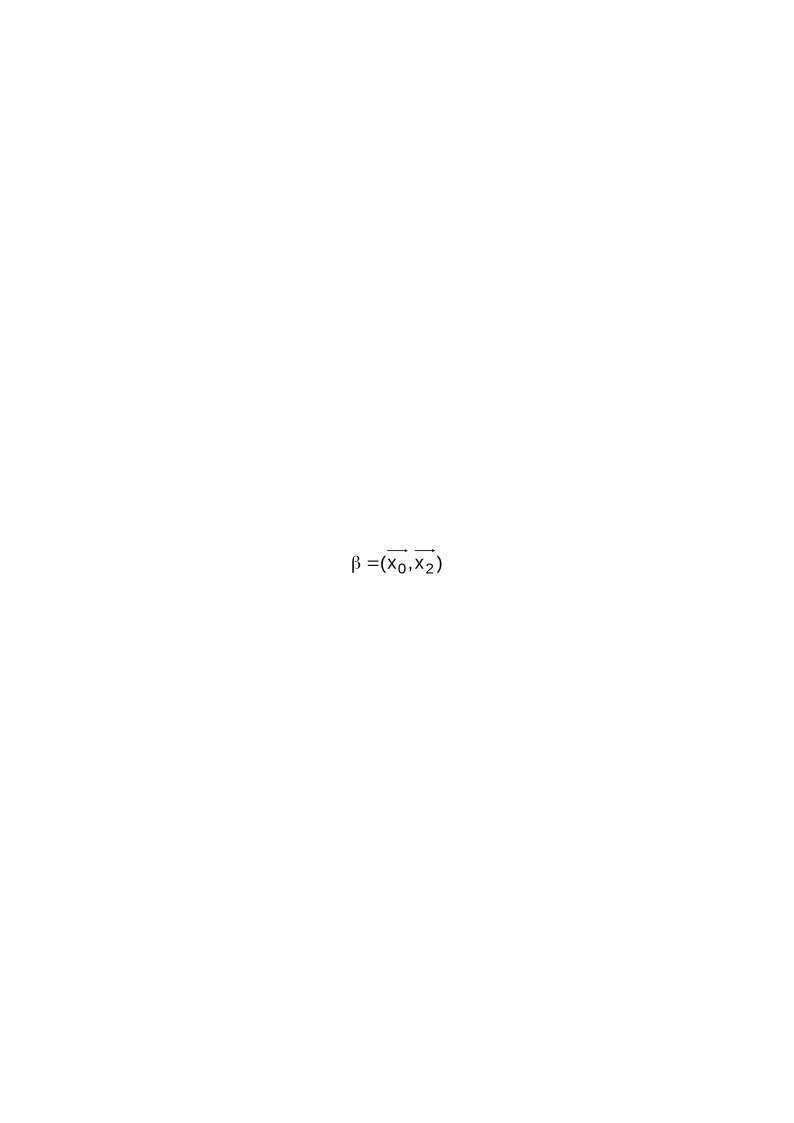
\includegraphics{images/image130.png}

Le mouvement de 1/3 est une rotation d'axe
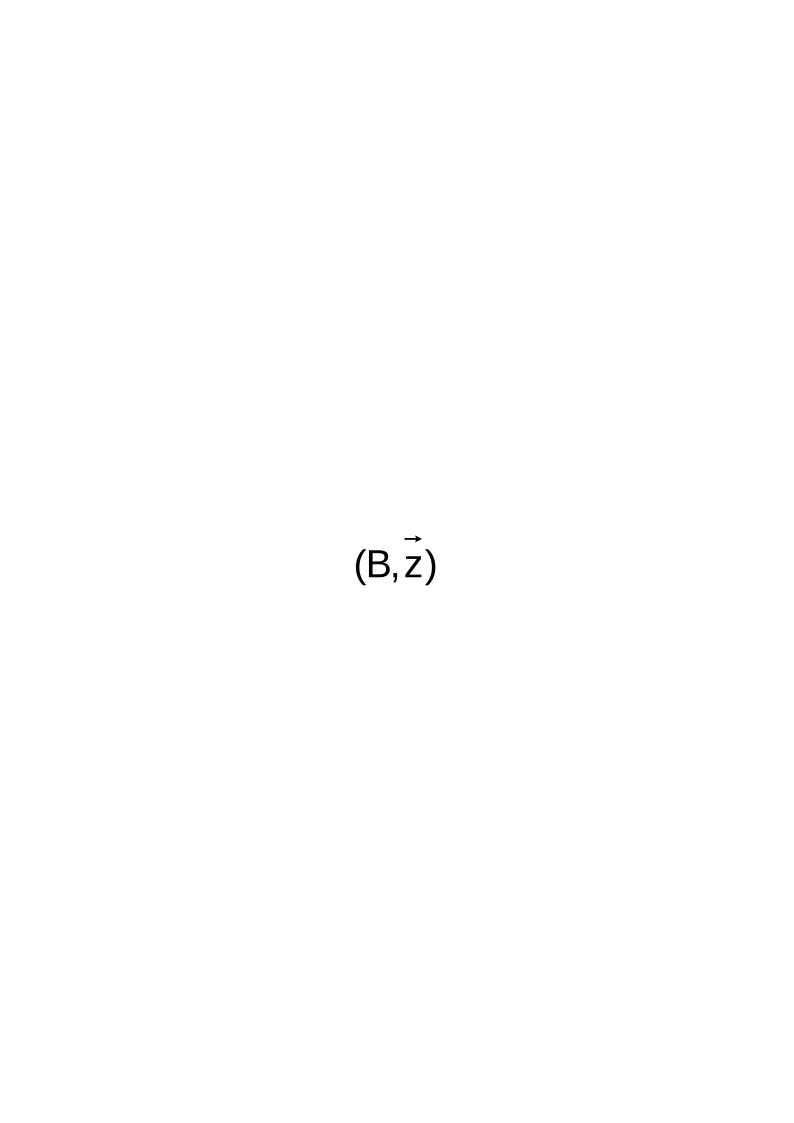
\includegraphics{images/image131.png}~

Le mouvement de 2/4 est une rotation d'axe
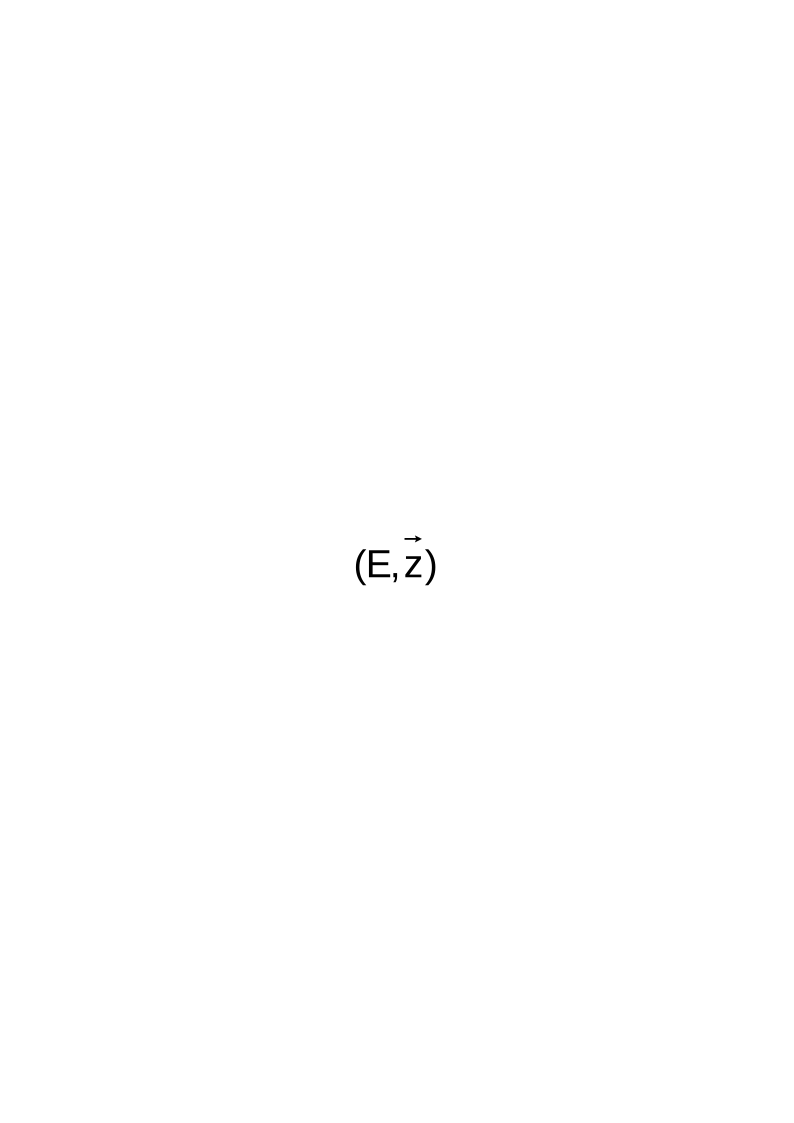
\includegraphics{images/image132.png}~

Le mouvement de 3/4 est une rotation d'axe
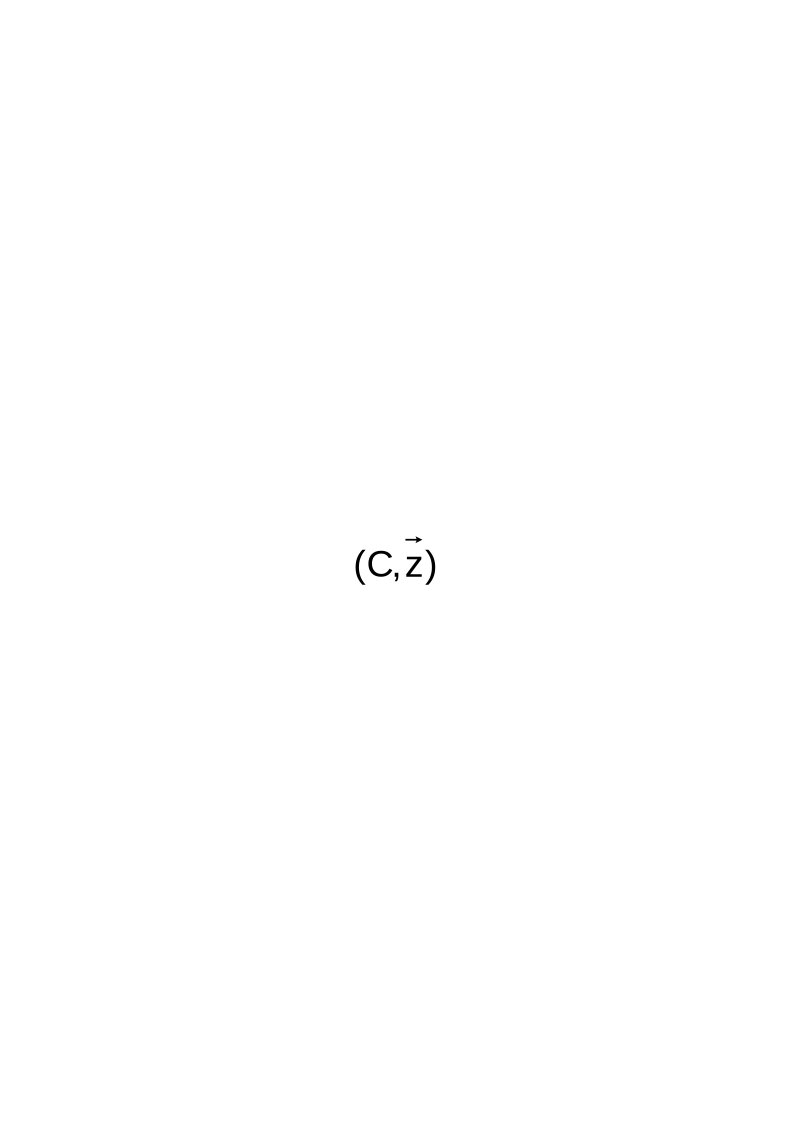
\includegraphics{images/image133.png}~

Par ailleurs~: 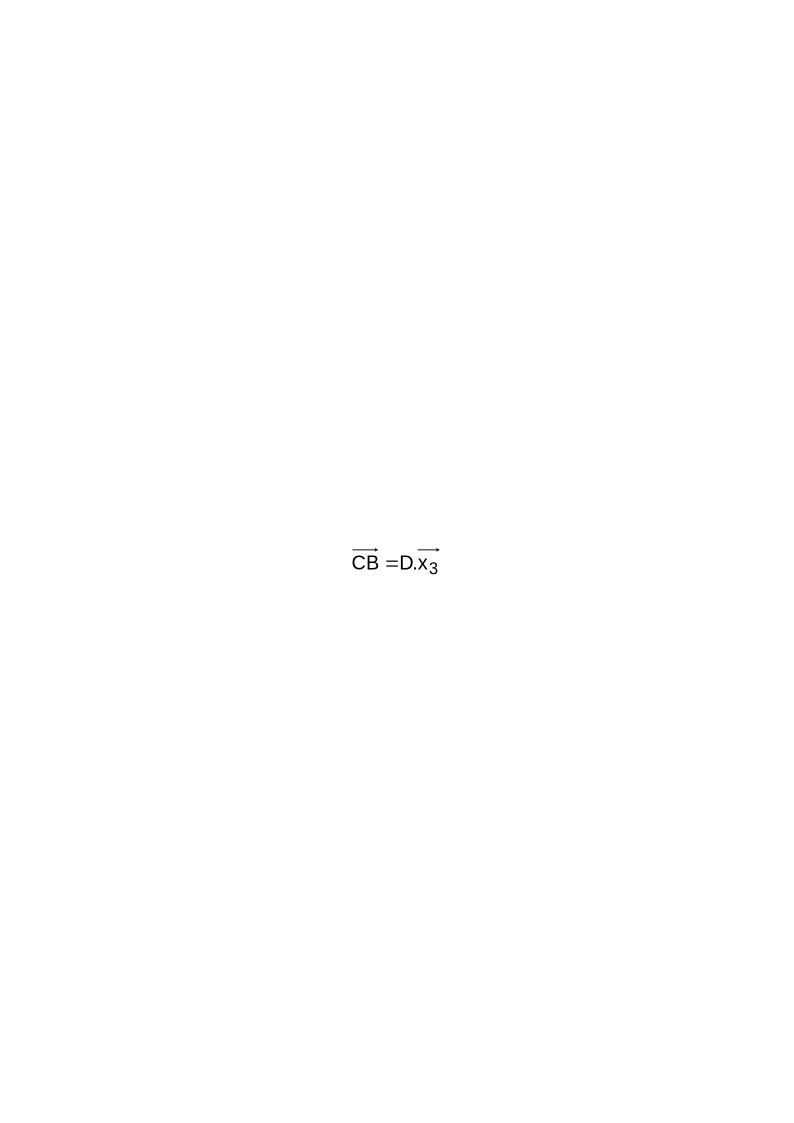
\includegraphics{images/image134.png},
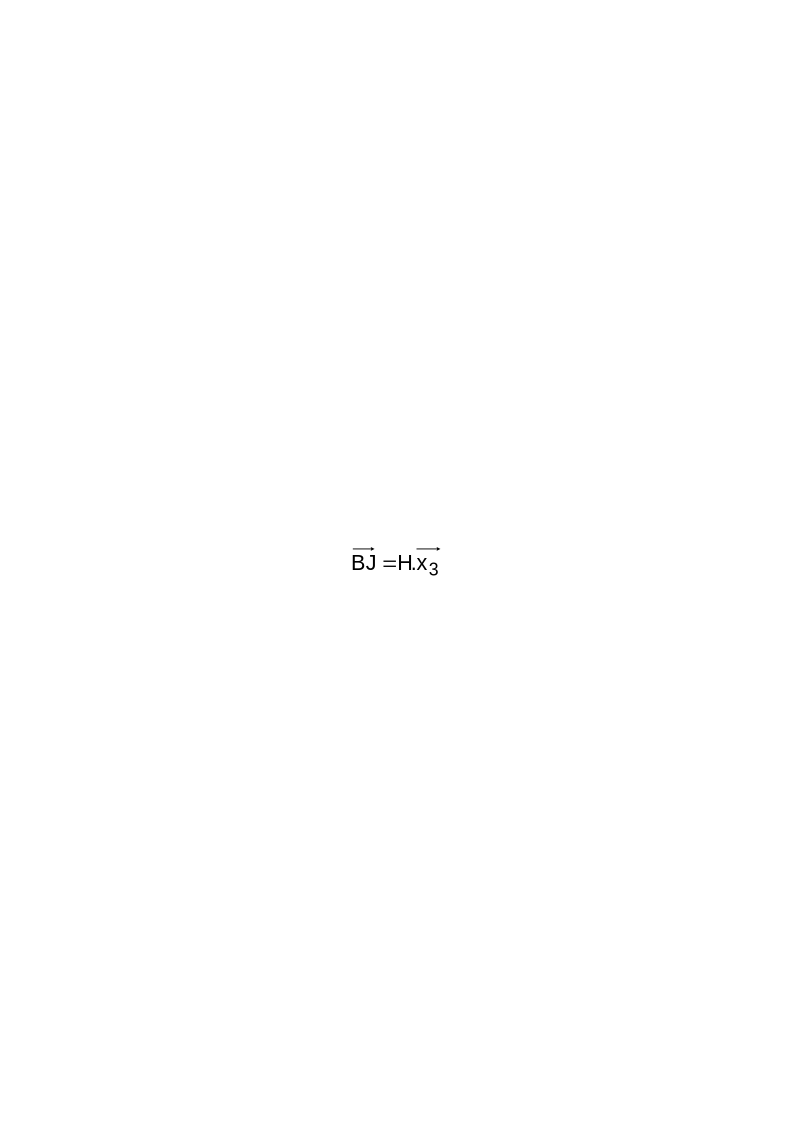
\includegraphics{images/image135.png},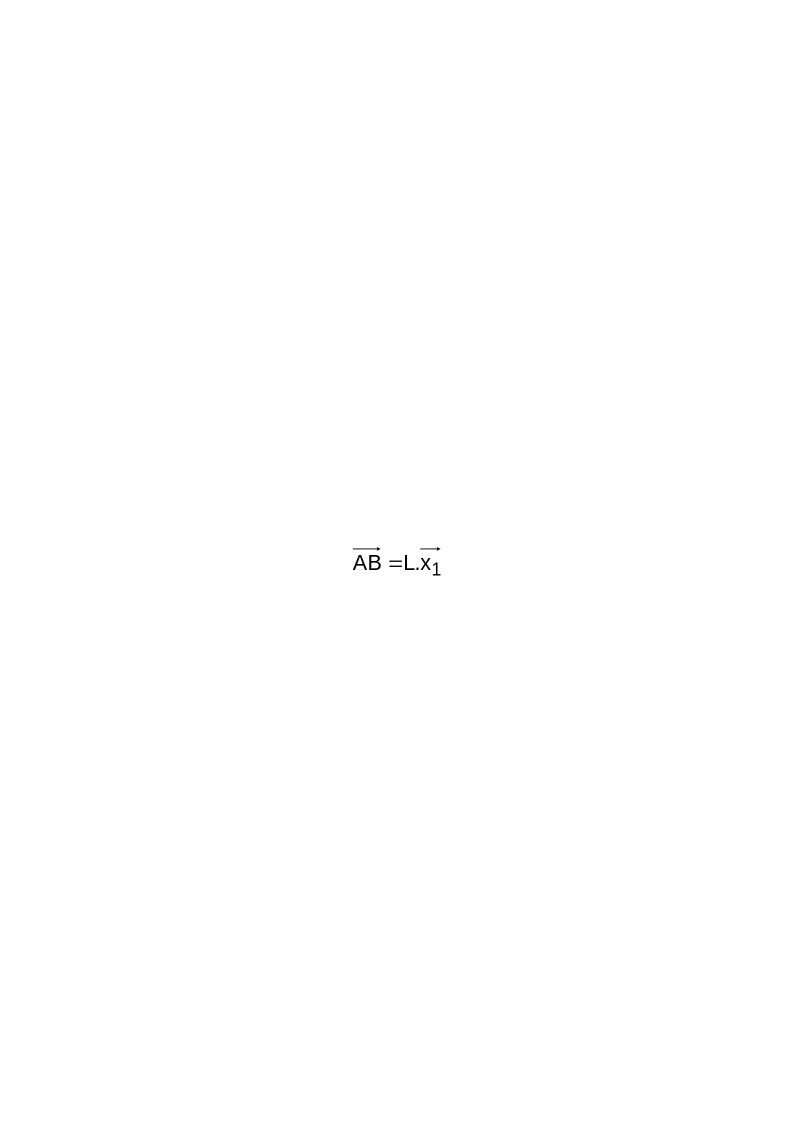
\includegraphics{images/image136.png},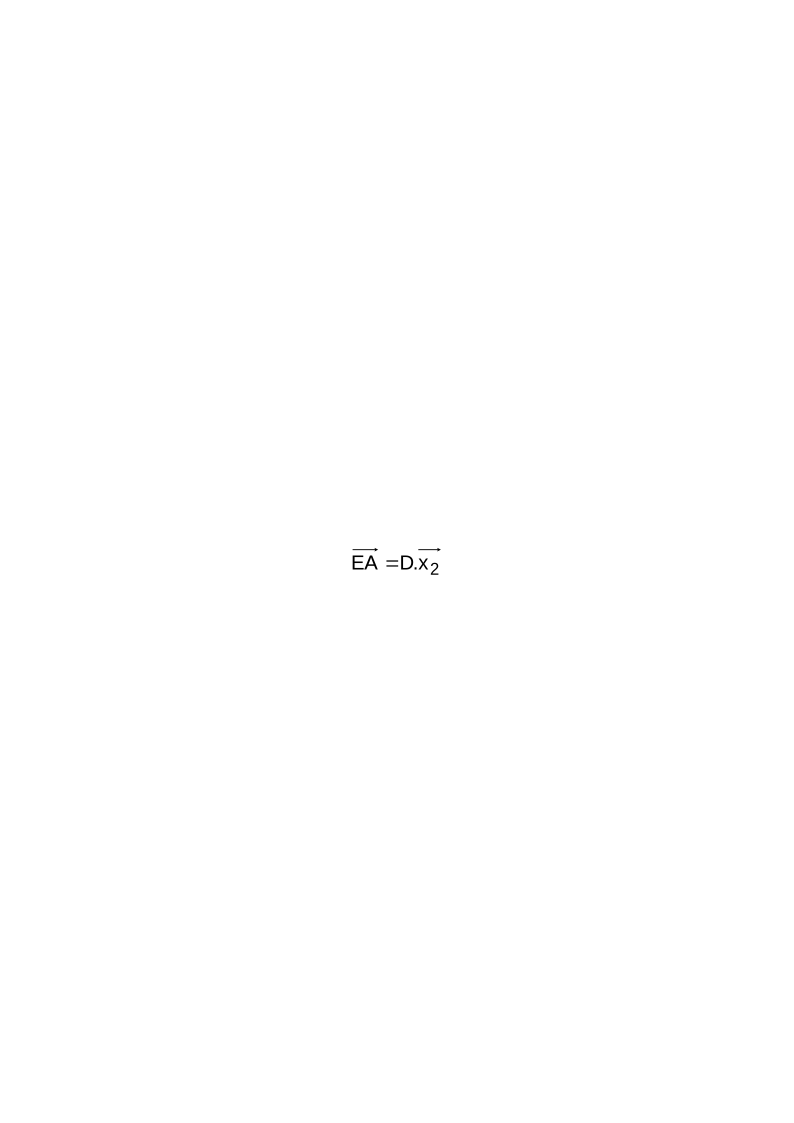
\includegraphics{images/image137.png}et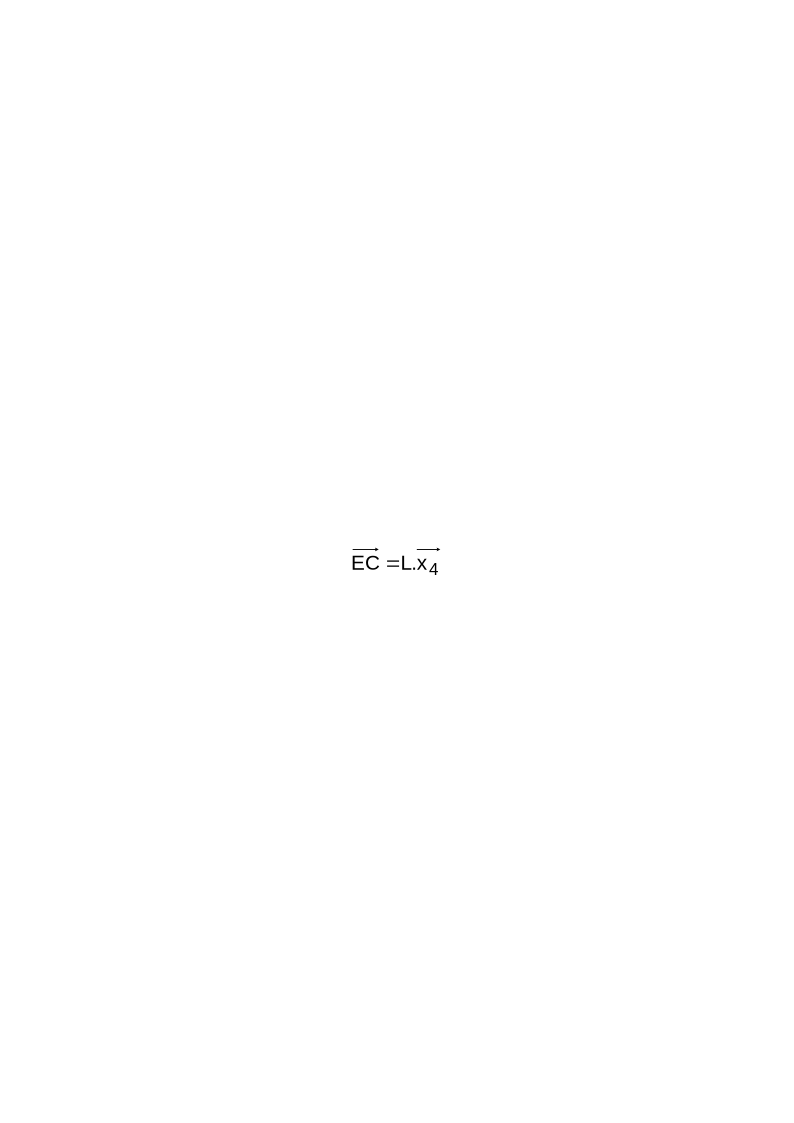
\includegraphics{images/image138.png}

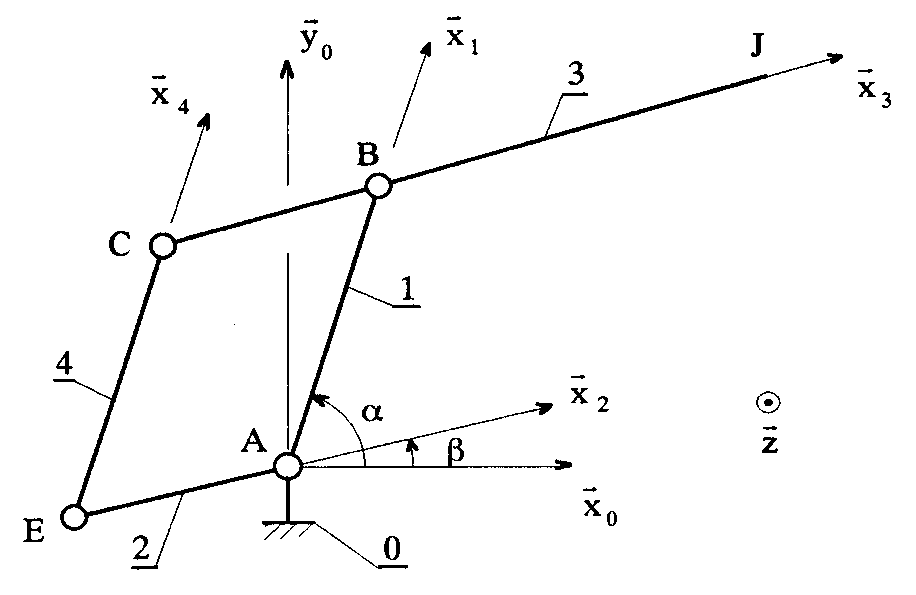
\includegraphics[width=\linewidth]{images/image139.png}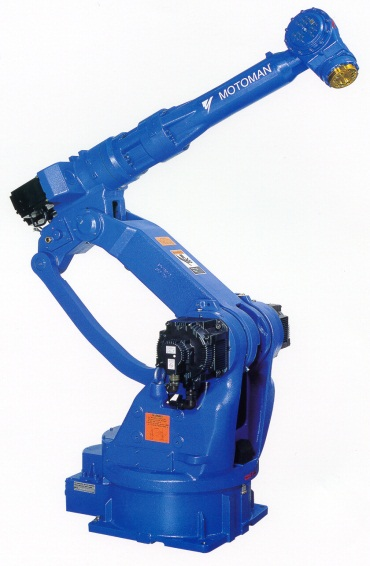
\includegraphics[width=\linewidth]{images/image140.jpeg}

\emph{figure 2}

\emph{figure 1}

\textbf{1 - Dessiner} les figures de changement de base. Essayer de
regrouper si possible.
\end{minipage} \\
\midrule\noalign{}
\endhead
\bottomrule\noalign{}
\endlastfoot
\end{longtable}

\section{LIAISON EQUIVALENTE}\label{liaison-equivalente}

Dans le but d'obtenir un schéma cinématique minimal, on est parfois
amené à chercher une \emph{\textbf{liaison équivalente à un ensemble de
plusieurs liaisons}}.

Cette étape pouvant se faire de manière intuitive dans les cas simples
ou en utilisant les torseurs cinématiques.

Une liaison équivalente à plusieurs liaisons entre deux CEC est une
liaison qui traduit le même mouvement relatif et qui permet de
transmettre les mêmes actions mécaniques.

\subsection{Analyse des mouvements possible avec une association de
liaisons}\label{analyse-des-mouvements-possible-avec-une-association-de-liaisons}

Il est possible de déterminer la liaison équivalente de plusieurs
liaisons en série ou en parallèle en analysant les seuls mouvements
possibles avec l'association des deux. Pour cela, il faut~:

\begin{enumerate}
\def\labelenumi{\arabic{enumi}.}
\item
  Identifier chaque liaison
\item
  Déterminer les degrés de liberté de chaque liaison seule (sans
  l'association de liaisons)
\item
  Travailler sur la liaison qui a le moins degrés de liberté et
  «~tester~» chacun de ses degrés de liberté pour savoir ceux qui sont
  possibles ou non avec l'association de liaison
\item
  Identifier la liaison équivalente avec les degrés de liberté restants
  et le repère associé.
\end{enumerate}

Exemple~: Déterminer la liaison équivalente suivante

\begin{longtable}[]{@{}
  >{\raggedright\arraybackslash}p{(\columnwidth - 8\tabcolsep) * \real{0.1849}}
  >{\raggedright\arraybackslash}p{(\columnwidth - 8\tabcolsep) * \real{0.1806}}
  >{\raggedright\arraybackslash}p{(\columnwidth - 8\tabcolsep) * \real{0.1935}}
  >{\raggedright\arraybackslash}p{(\columnwidth - 8\tabcolsep) * \real{0.2065}}
  >{\raggedright\arraybackslash}p{(\columnwidth - 8\tabcolsep) * \real{0.2344}}@{}}
\toprule\noalign{}
\begin{minipage}[b]{\linewidth}\raggedright
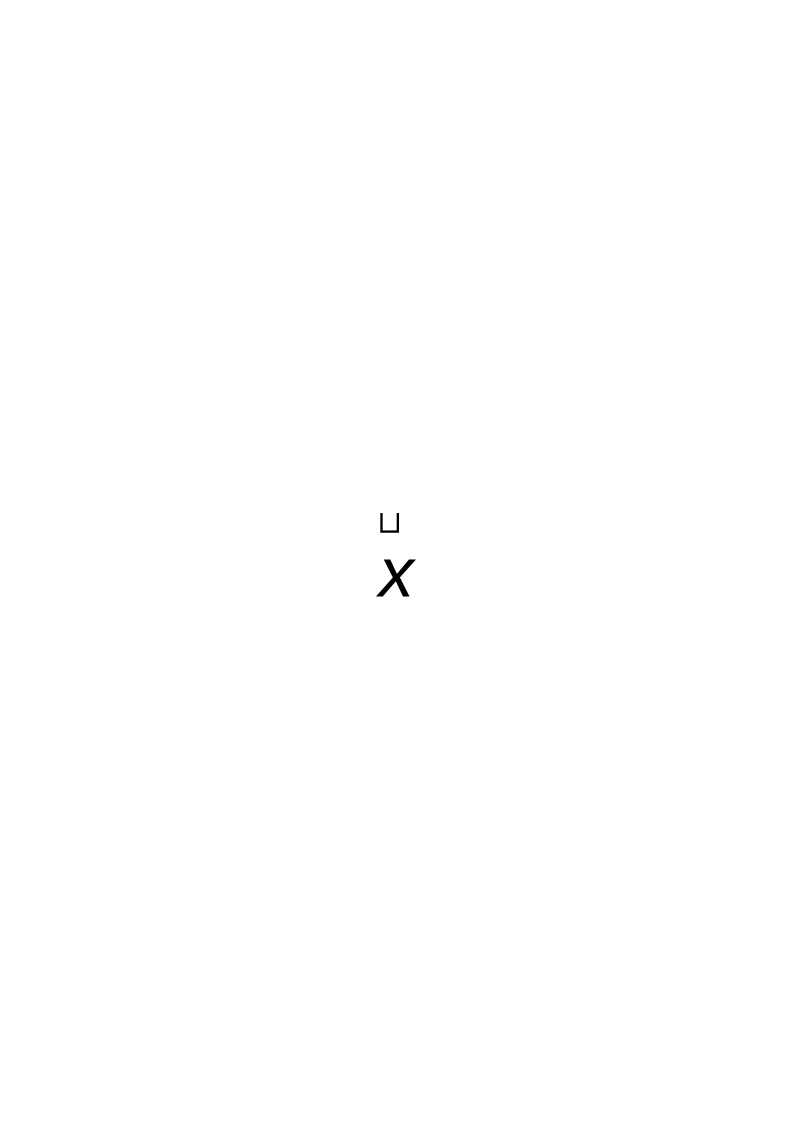
\includegraphics{images/image141.png}

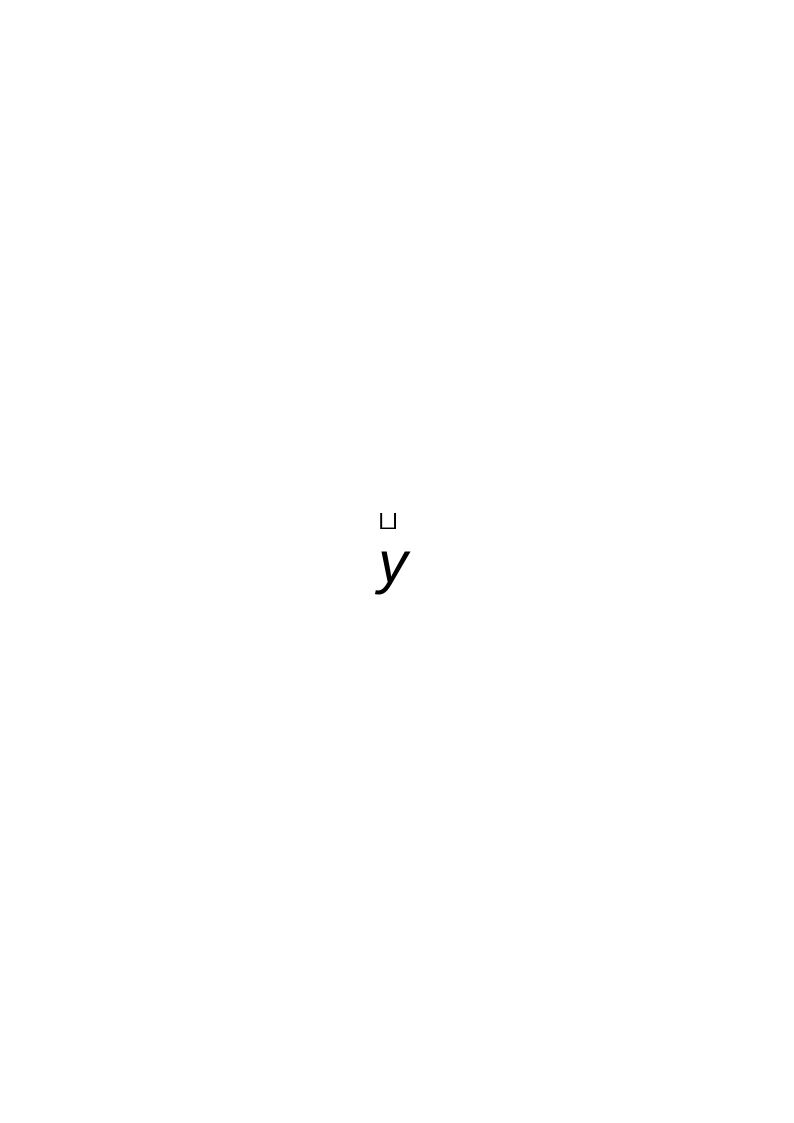
\includegraphics{images/image142.png}

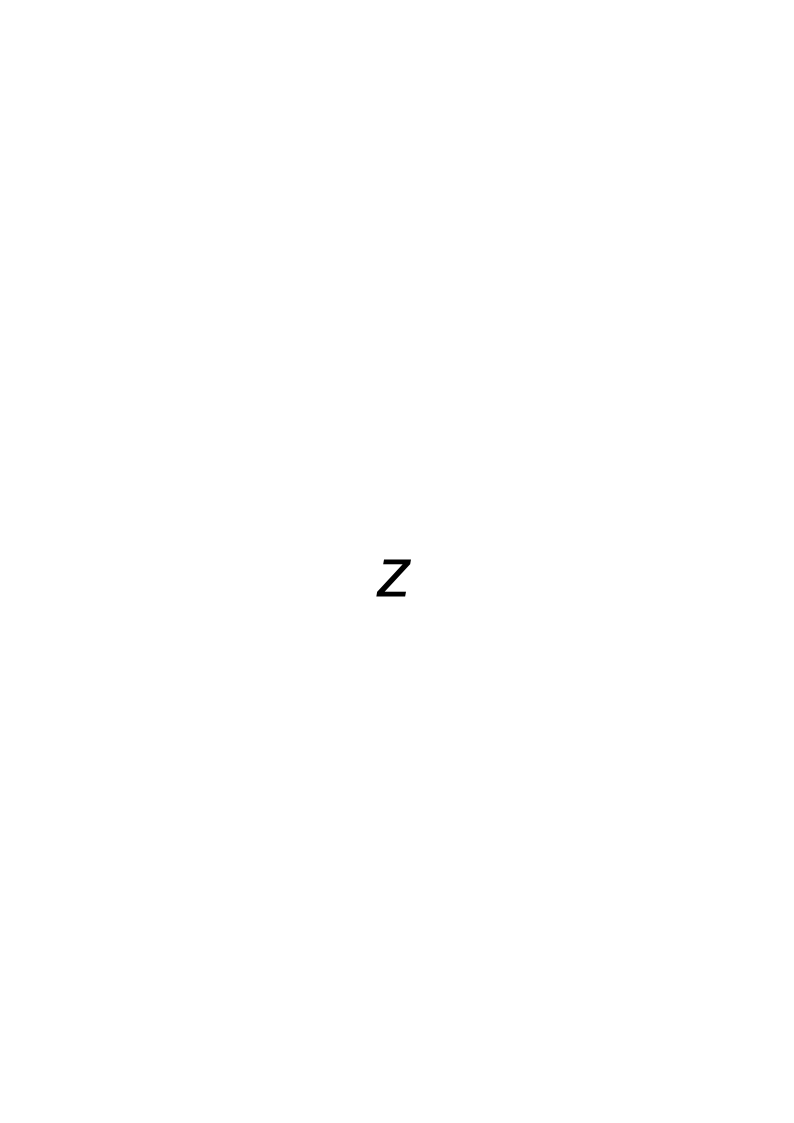
\includegraphics{images/image143.png}

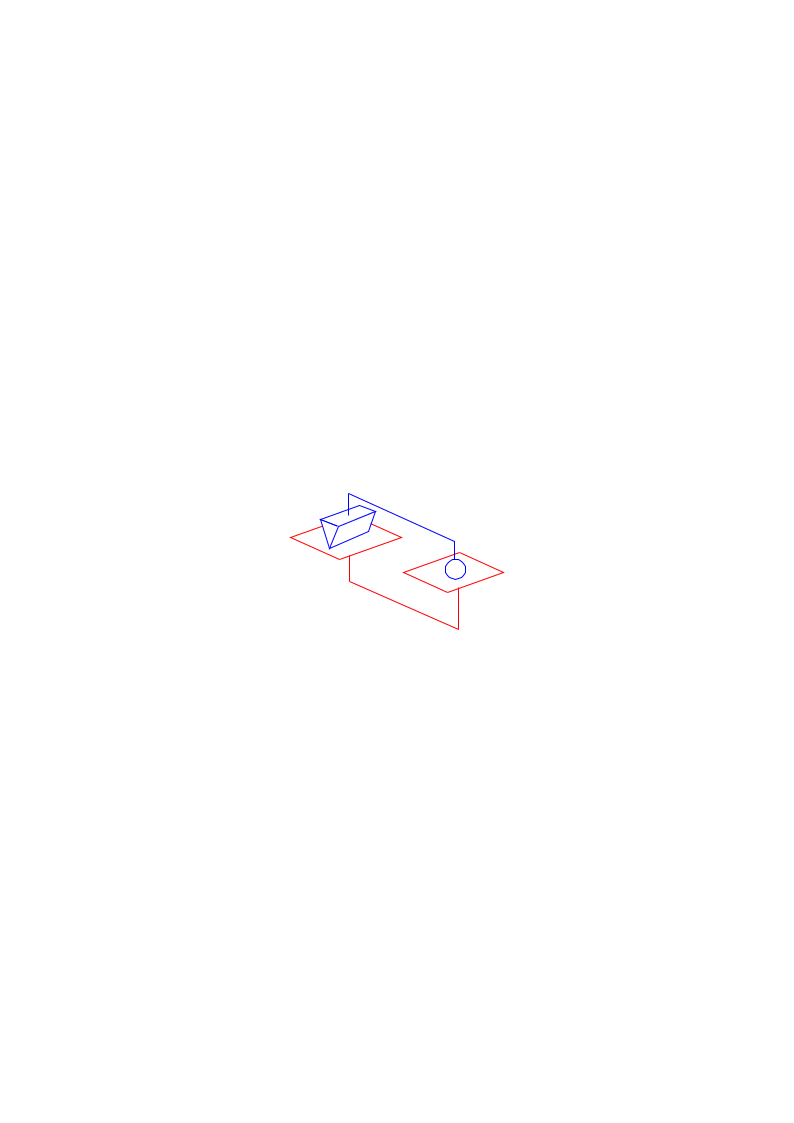
\includegraphics{images/image144.png}
\end{minipage} & \begin{minipage}[b]{\linewidth}\raggedright
1.

Liaison à gauche~: linéaire rectiligne de normale y et de contact z

Liaison à droite~: ponctuelle de normale y
\end{minipage} & \begin{minipage}[b]{\linewidth}\raggedright
2.

Liaison à gauche~:

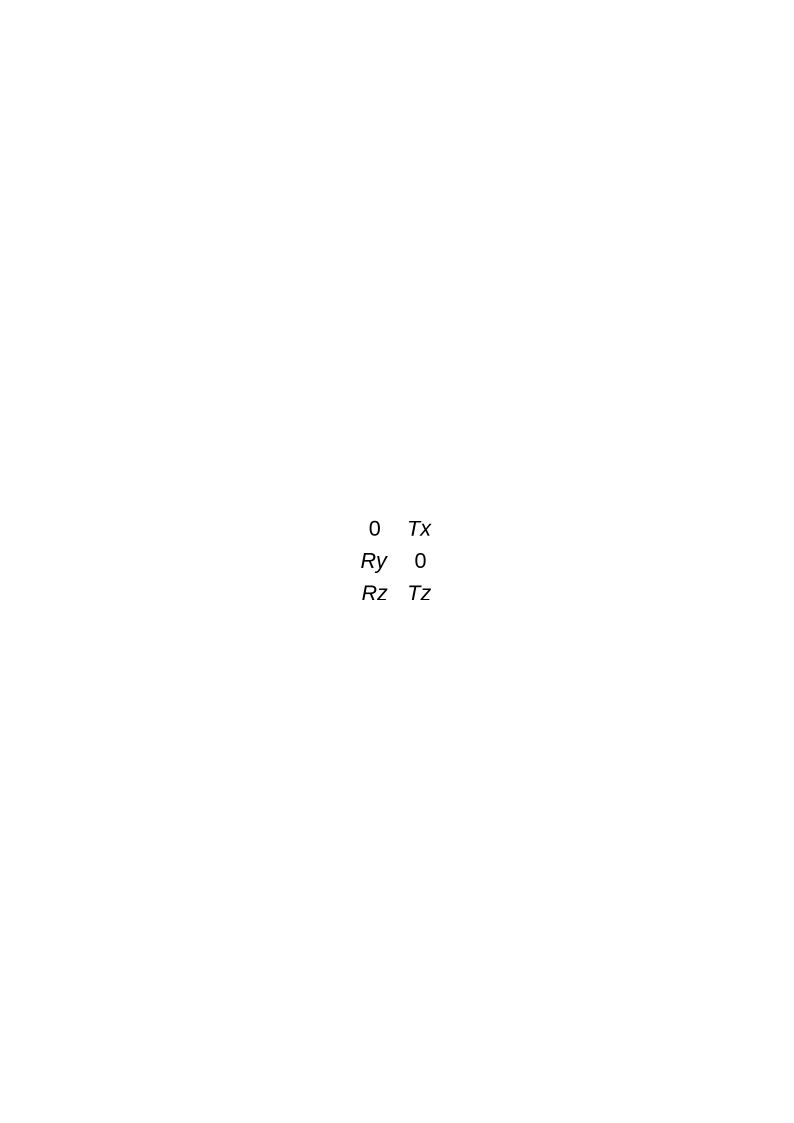
\includegraphics{images/image145.png}

Liaison à droite~:

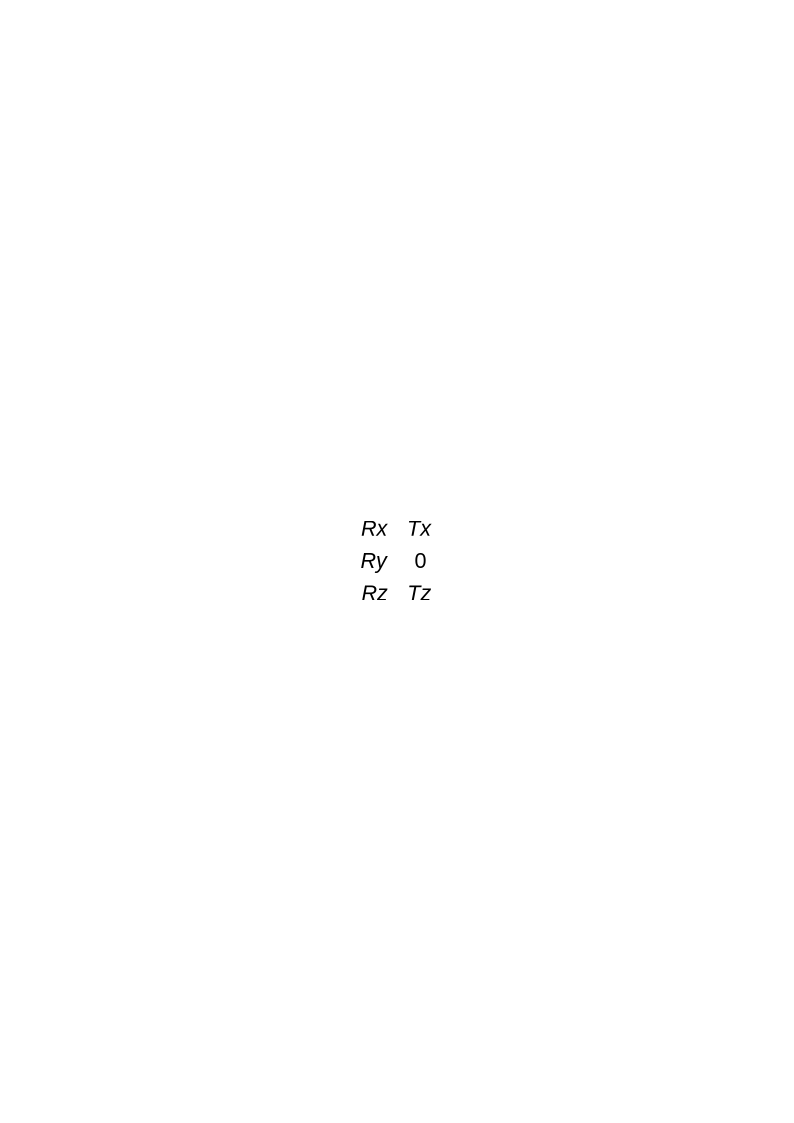
\includegraphics{images/image146.png}
\end{minipage} & \begin{minipage}[b]{\linewidth}\raggedright
3. La linéaire rectiligne est celle qui a le moins de degré de liberté.

L'association des deux empêche la rotation suivant z (Rz)

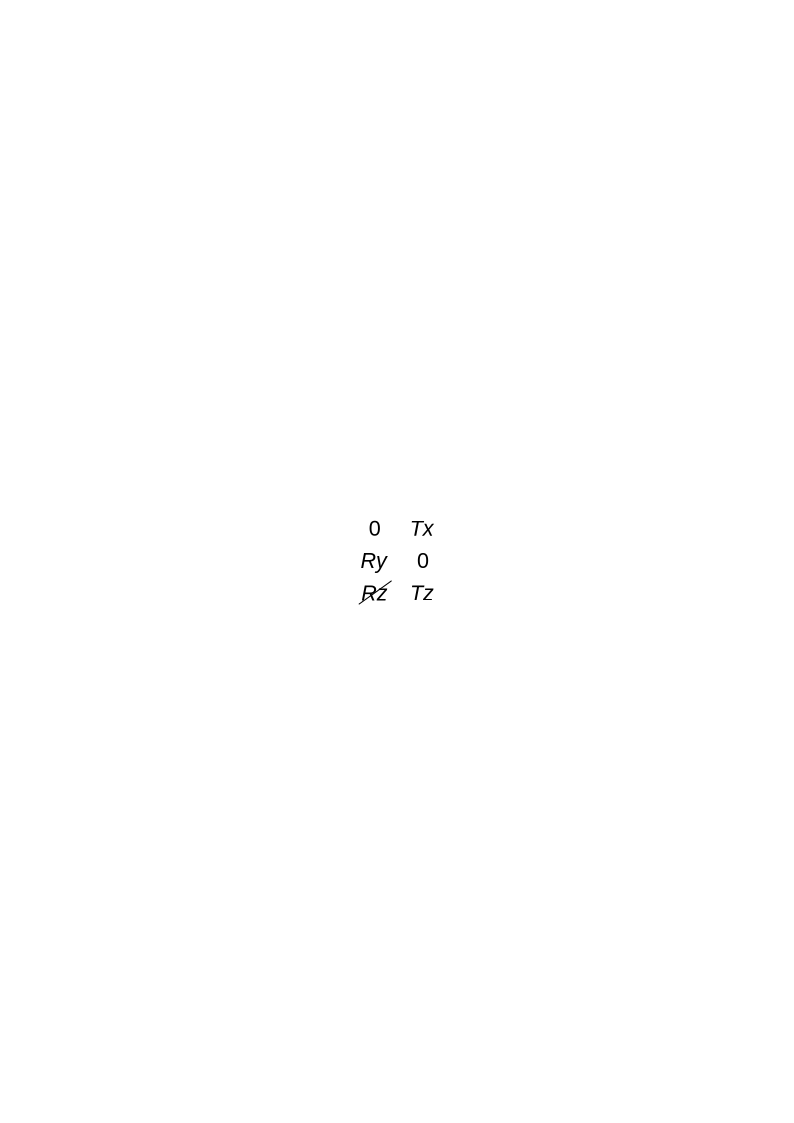
\includegraphics{images/image147.png}
\end{minipage} & \begin{minipage}[b]{\linewidth}\raggedright
4. On identifie une liaison équivalente appui-plan de normale y~:

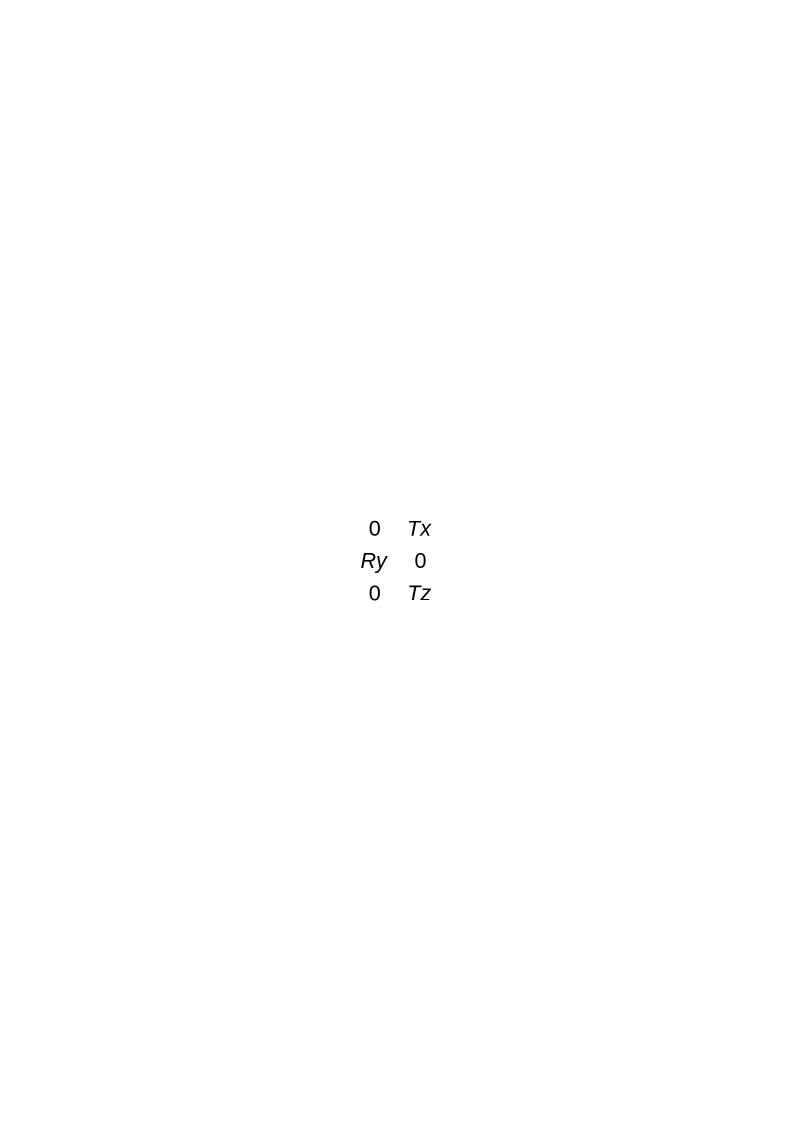
\includegraphics{images/image148.png}

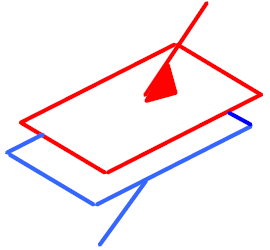
\includegraphics[width=\linewidth]{images/image149.png}
\end{minipage} \\
\midrule\noalign{}
\endhead
\bottomrule\noalign{}
\endlastfoot
\end{longtable}

\subsection*{}\label{section}
\addcontentsline{toc}{subsubsection}{}


\includegraphics[width=\linewidth]{images/image150.png}

\subsection{Liaisons en parallèle avec les
torseurs}\label{liaisons-en-paralluxe8le-avec-les-torseurs}

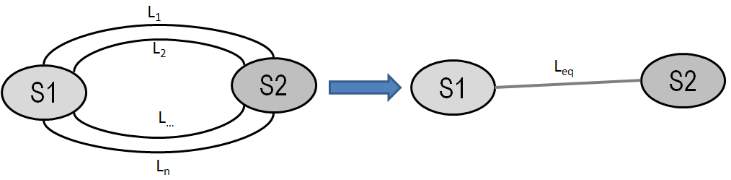
\includegraphics[width=\linewidth]{images/image151.png}Les
\emph{\textbf{n}} liaisons \emph{\textbf{L\textsubscript{1}}},
\emph{\textbf{L\textsubscript{2}}},\ldots.\emph{\textbf{L\textsubscript{n}}}
sont dites «~\emph{\textbf{en parallèles}}~» si elles relient
directement deux CEC \emph{\textbf{S1}} et \emph{\textbf{S2}} sur le
graphe des liaisons.

La liaison équivalente, notée \emph{\textbf{L\textsubscript{eq}}}, est
identifiée à partir de la forme de son torseur cinématique qui est tel
que~:

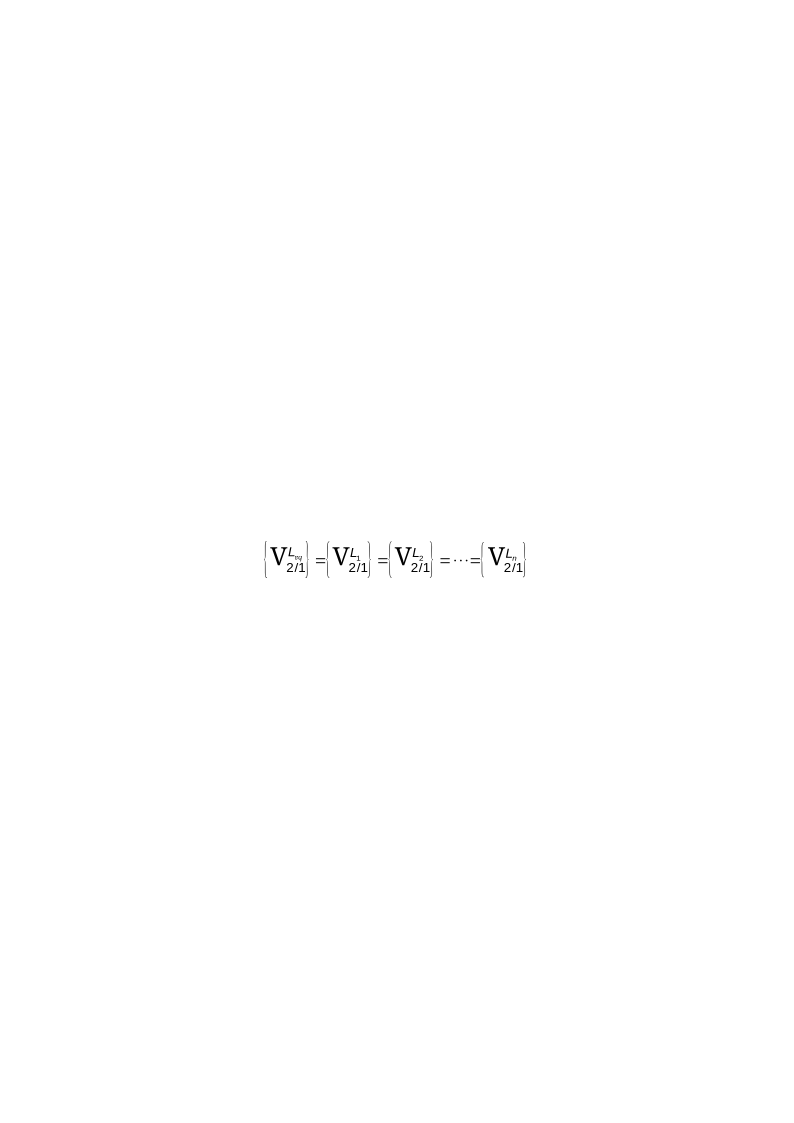
\includegraphics{images/image152.png}

En effet, puisqu'elle doit traduire le même mouvement relatif entre les
deux CEC, \emph{\textbf{le}} \emph{\textbf{torseur de la liaison
équivalente doit être «~compatible~» avec les torseurs cinématiques des
n liaisons}}.

\subsection{Liaisons en série avec les
torseurs}\label{liaisons-en-suxe9rie-avec-les-torseurs}

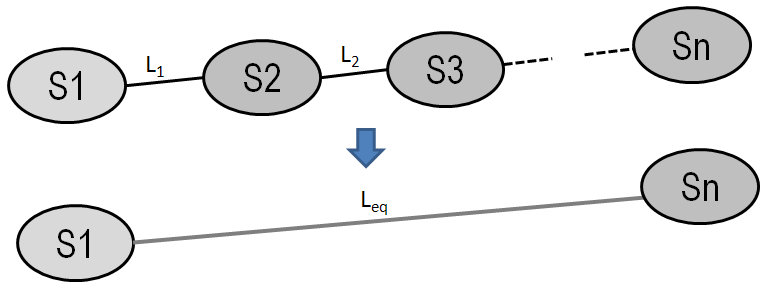
\includegraphics[width=\linewidth]{images/image153.png}Les
\emph{\textbf{n}} liaisons \emph{\textbf{L\textsubscript{1}}},
\emph{\textbf{L\textsubscript{2}}},\ldots.\emph{\textbf{L\textsubscript{n}}}
sont dites «~\emph{\textbf{en série}}~» entre deux CEC
\emph{\textbf{S1}} et \emph{\textbf{Sn}} si elles sont disposées, sur le
graphe des liaisons, à la suite l'une de l'autre par l'intermédiaire de
\emph{\textbf{(n-1)}} CEC.

Par \emph{\textbf{composition des torseurs cinématique}}, on a~:

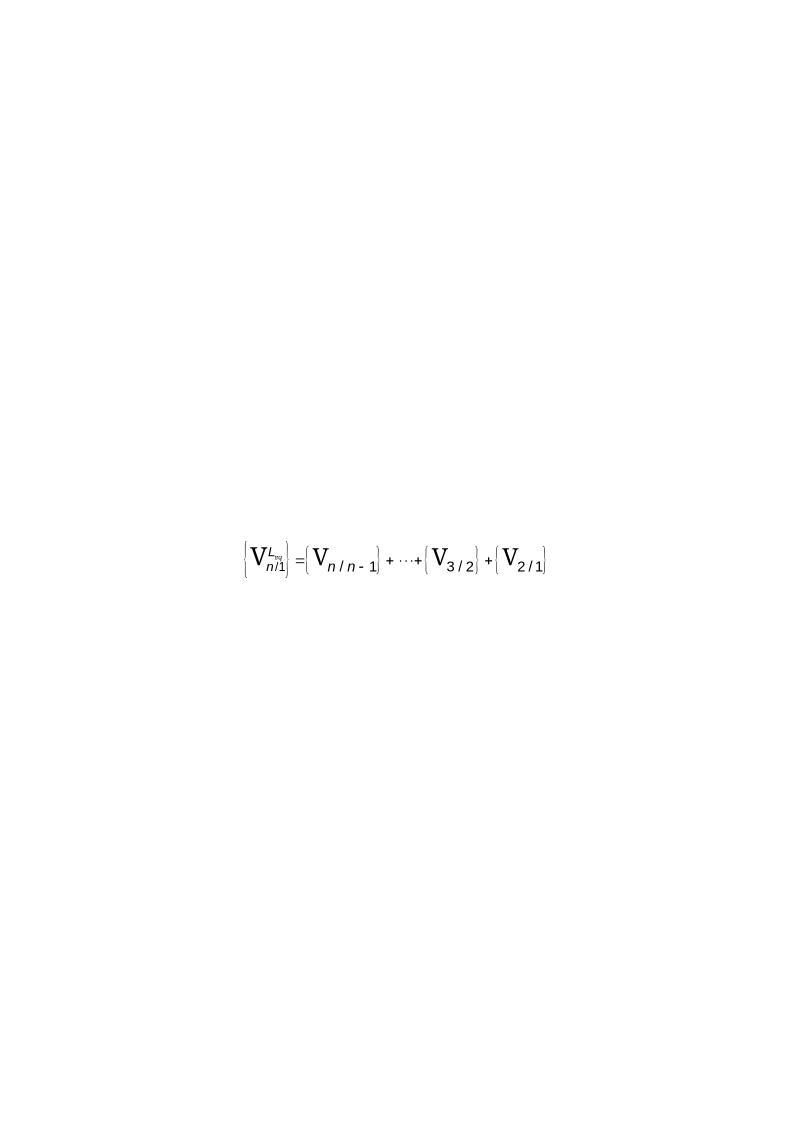
\includegraphics{images/image154.png}

En effet, la liaison équivalente présente les degrés de liberté qui
n'ont été supprimés par aucune des \emph{\textbf{n}} liaisons.

\section{Sources}\label{sources}

Ce cours a été élaboré à l'aide de nombreuses ressources~provenant de
différents collègues~: Jacques Le Goff, Corentin Kerzreho, Stéphane
Génouel, de documents publics d'industriels, des activités pédagogiques
de collègues de l'UPSTI.

\section{Exercices du chapitre}\label{exercices-du-chapitre}


\includegraphics[width=\linewidth]{images/image155.png}

\textbf{APPLICATIONS GRAPHE DE LIAISONS}


\includegraphics[width=\linewidth]{images/image156.png}
Niveau 2

\begin{enumerate}
\def\labelenumi{\arabic{enumi}.}
\item
  Donner les graphes de laisons des systèmes suivants
\end{enumerate}

\textbf{Bielle-manivelle}

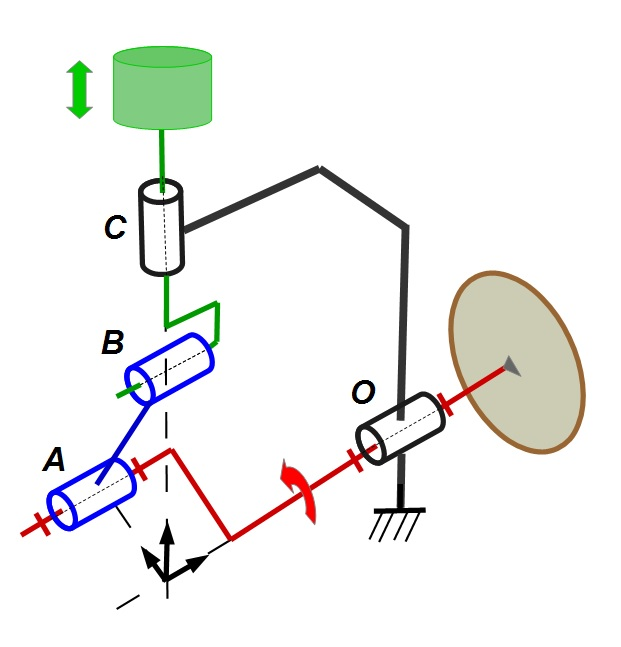
\includegraphics[width=\linewidth]{images/image157.jpeg}

\textbf{Lève-Personne}

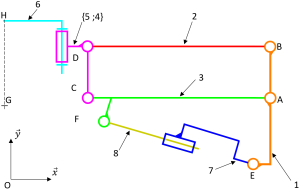
\includegraphics[width=\linewidth]{images/image158.png}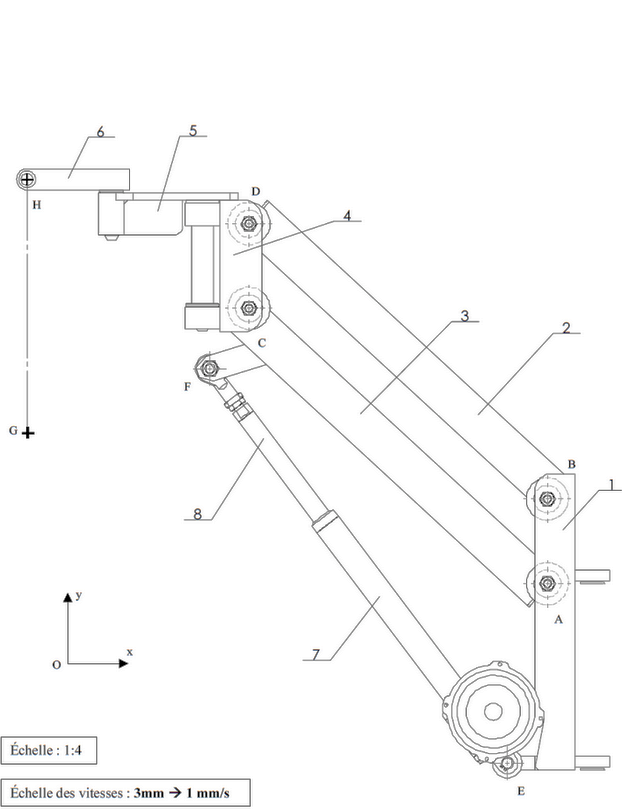
\includegraphics[width=\linewidth]{images/image159.png}

\textbf{Système Spiralift pour salles modulables}

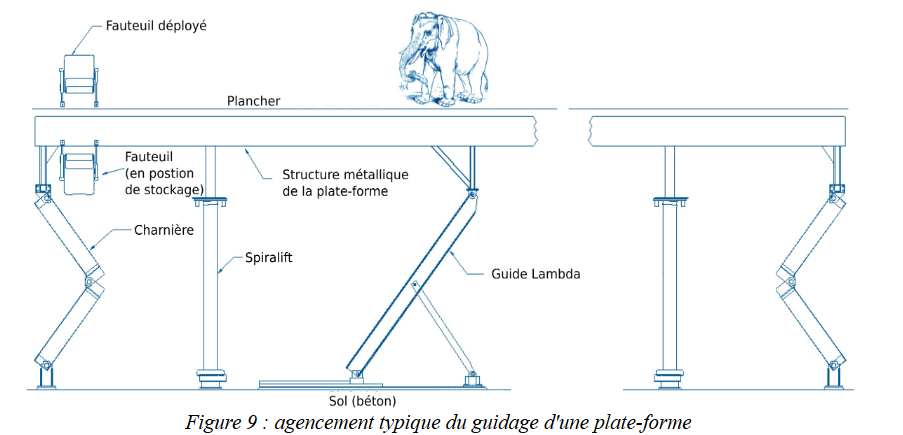
\includegraphics[width=\linewidth]{images/image160.png}

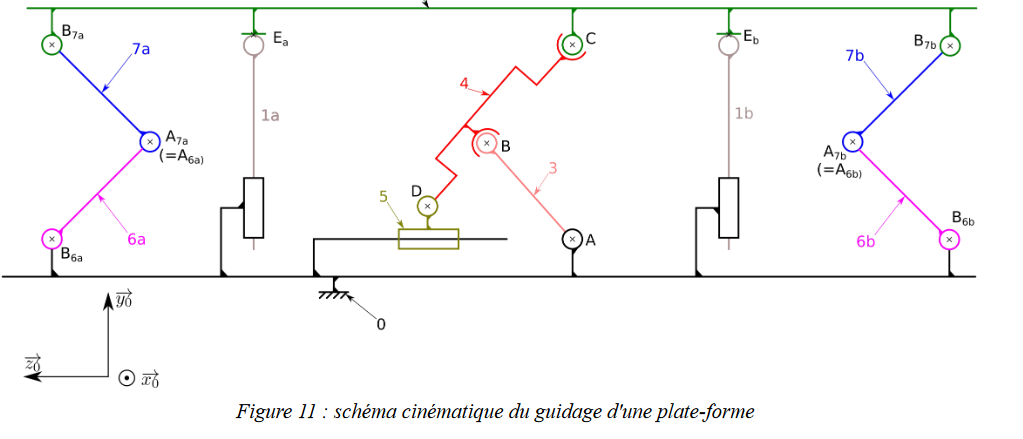
\includegraphics[width=\linewidth]{images/image161.png}

\textbf{Dépose de bagages automatisés}


\includegraphics[width=\linewidth]{images/image162.emf}
\includegraphics[width=\linewidth]{images/image163.emf}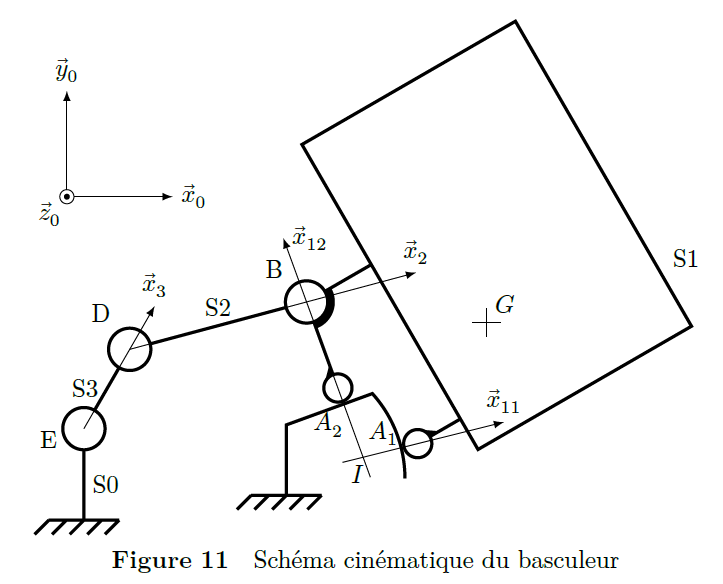
\includegraphics[width=\linewidth]{images/image164.png}

\textbf{Robot manipulateur}

\begin{longtable}[]{@{}
  >{\raggedright\arraybackslash}p{(\columnwidth - 2\tabcolsep) * \real{0.3640}}
  >{\raggedright\arraybackslash}p{(\columnwidth - 2\tabcolsep) * \real{0.6360}}@{}}
\toprule\noalign{}
\begin{minipage}[b]{\linewidth}\raggedright
\begin{quote}
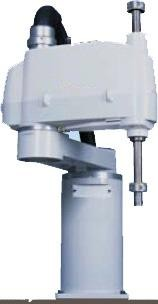
\includegraphics[width=\linewidth]{images/image165.jpeg}
\end{quote}
\end{minipage} & \begin{minipage}[b]{\linewidth}\raggedright
\begin{quote}
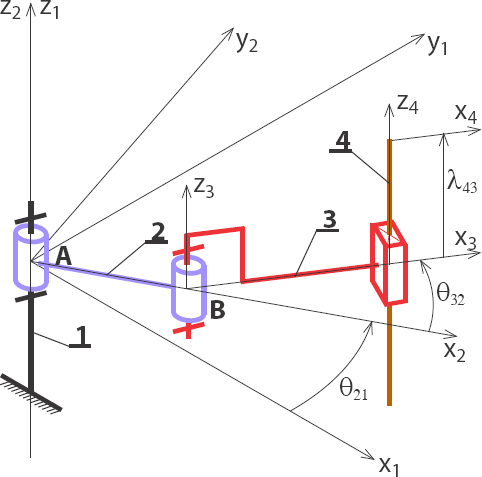
\includegraphics[width=\linewidth]{images/image166.png}
\end{quote}
\end{minipage} \\
\midrule\noalign{}
\endhead
\bottomrule\noalign{}
\endlastfoot
\end{longtable}

\textbf{PERFORATRICE}


\includegraphics[width=\linewidth]{images/image156.png}
Niveau 1

\textbf{\ul{Objectif de l'étude~:}}

\begin{itemize}
\item
  \textbf{Modéliser} la perforatrice.
\end{itemize}

\begin{enumerate}
\item
  Mise en situation
\end{enumerate}

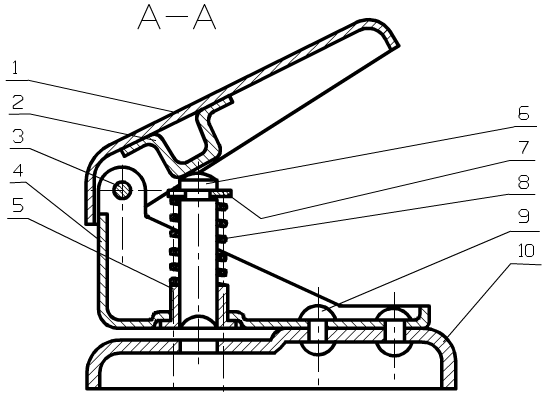
\includegraphics[width=\linewidth]{images/image167.png}

\textbf{Q1.} Repérer les classes d\textquotesingle équivalences en les
coloriant chacune avec une couleur différente. Lister les pièces qui
constituent ces classes

\textbf{Q2.} Dessiner le graphe des liaisons.

\begin{quote}
\textbf{PORTIQUE DE MANIPULATION}
\end{quote}


\includegraphics[width=\linewidth]{images/image156.png}
Niveau 3

\begin{enumerate}
\setcounter{enumi}{1}
\item
  Mise en situation
\end{enumerate}

Le mécanisme étudié est un portique de manipulation conçu et fabriqué
par la société A.V.M. Automation. Ce portique permet le transfert et la
rotation d`une pièce entre deux positions (voir \textbf{DT 01}). La
répétabilité du système (précision de positionnement) est inférieure à
0,05 mm. L'objet de notre étude est la pince de préhension et le guidage
du manipulateur Y (axe horizontal). Le document DT 01 présente le
portique de manipulation.

Le manipulateur de l'axe Z est actionné par un vérin pneumatique double
effet sans tige. Les manipulateurs des axes Y et Z sont actionnés par
des vérins pneumatiques double effet. Le rotatif Z est actionné par un
vérin pneumatique double effet et un ensemble pignon-crémaillère. La
pince de préhension est une pince parallèle actionnée par un vérin
pneumatique double effet. Pour chaque axe, il est possible d'ajouter des
positions intermédiaires (non représentées ici).

\[\overrightarrow{x}\]

\[\overrightarrow{z}\]

\[\overrightarrow{y}\]

O

\textbf{Zone d'étude 1}

Manipulateur Y

axe Y

Pince de préhension

Manipulateur X

axe X

Manipulateur Z

axe Z

Rotatif

axe Z

Bâti

fixe

\begin{enumerate}
\setcounter{enumi}{2}
\item
  Activités
\end{enumerate}

\begin{enumerate}
\def\labelenumi{\arabic{enumi}.}
\item
  Donner le schéma cinématique du manipulateur de l'axe Y à partir de
  l'éclaté (DT04).
\item
  Donner la liaison équivalente du manipulateur Y.
\item
  En déduire le schéma cinématique dans le plan et dans l'espace pour le
  portique de manipulation
\end{enumerate}

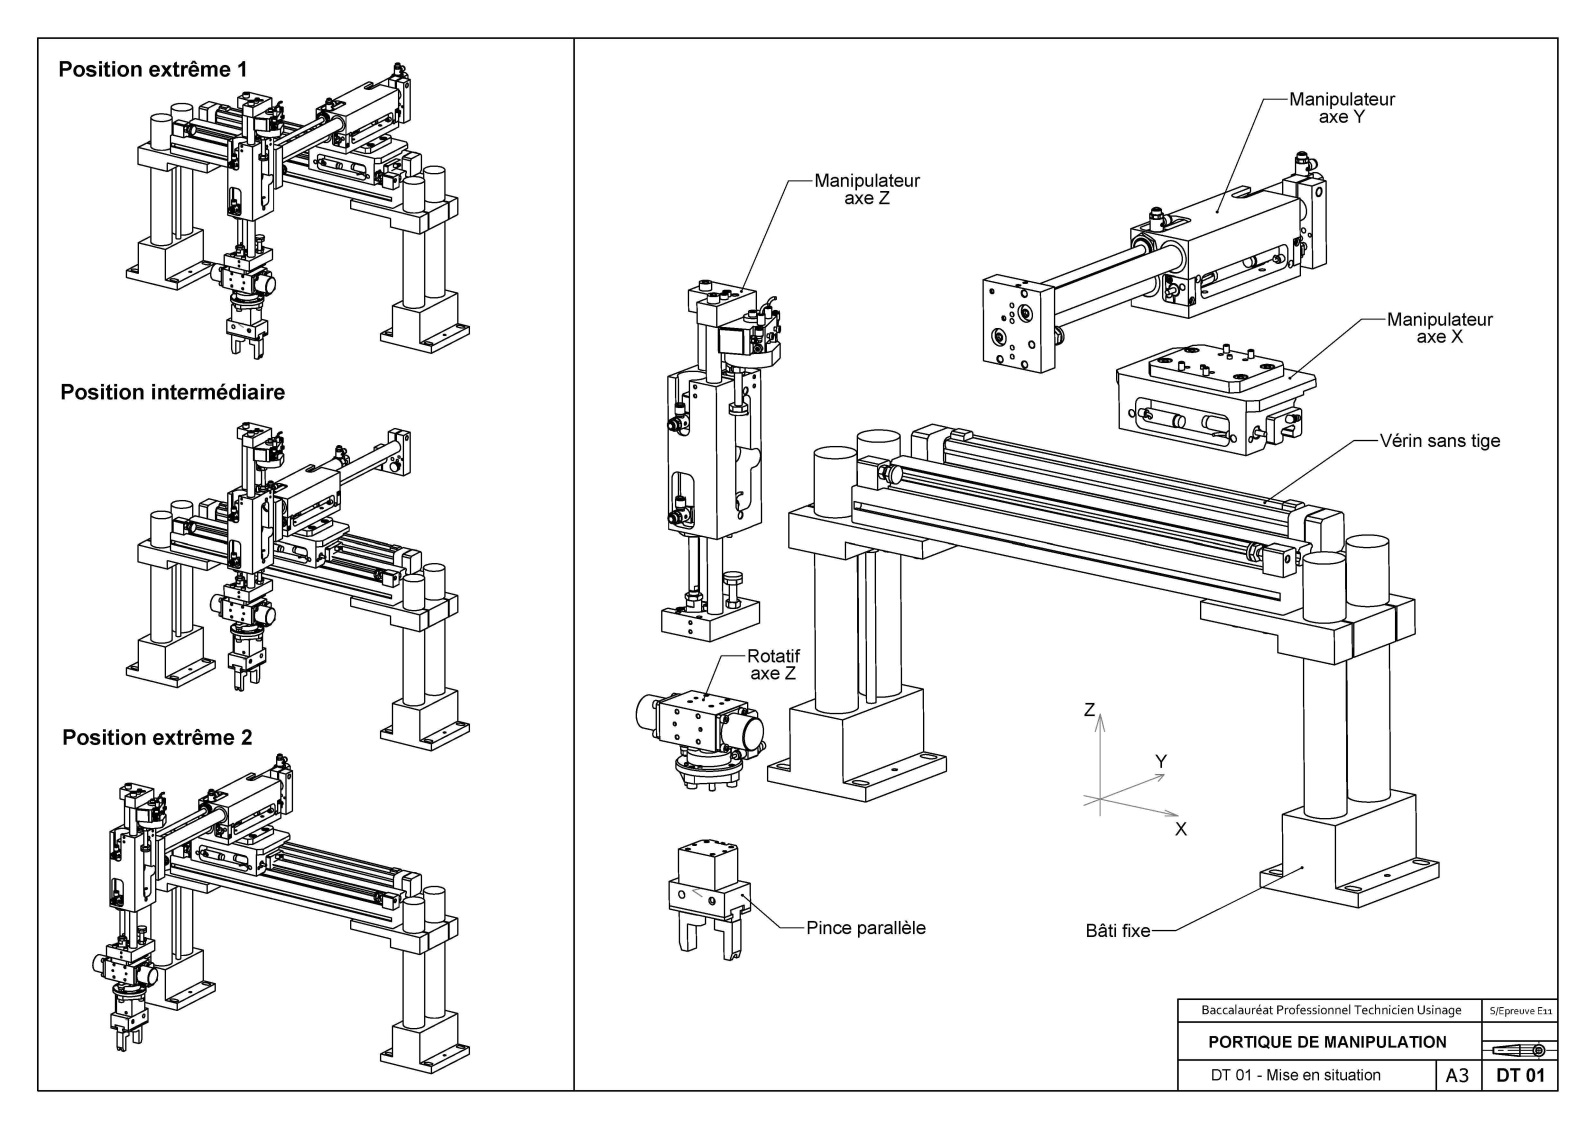
\includegraphics[width=\linewidth]{images/image172.jpeg}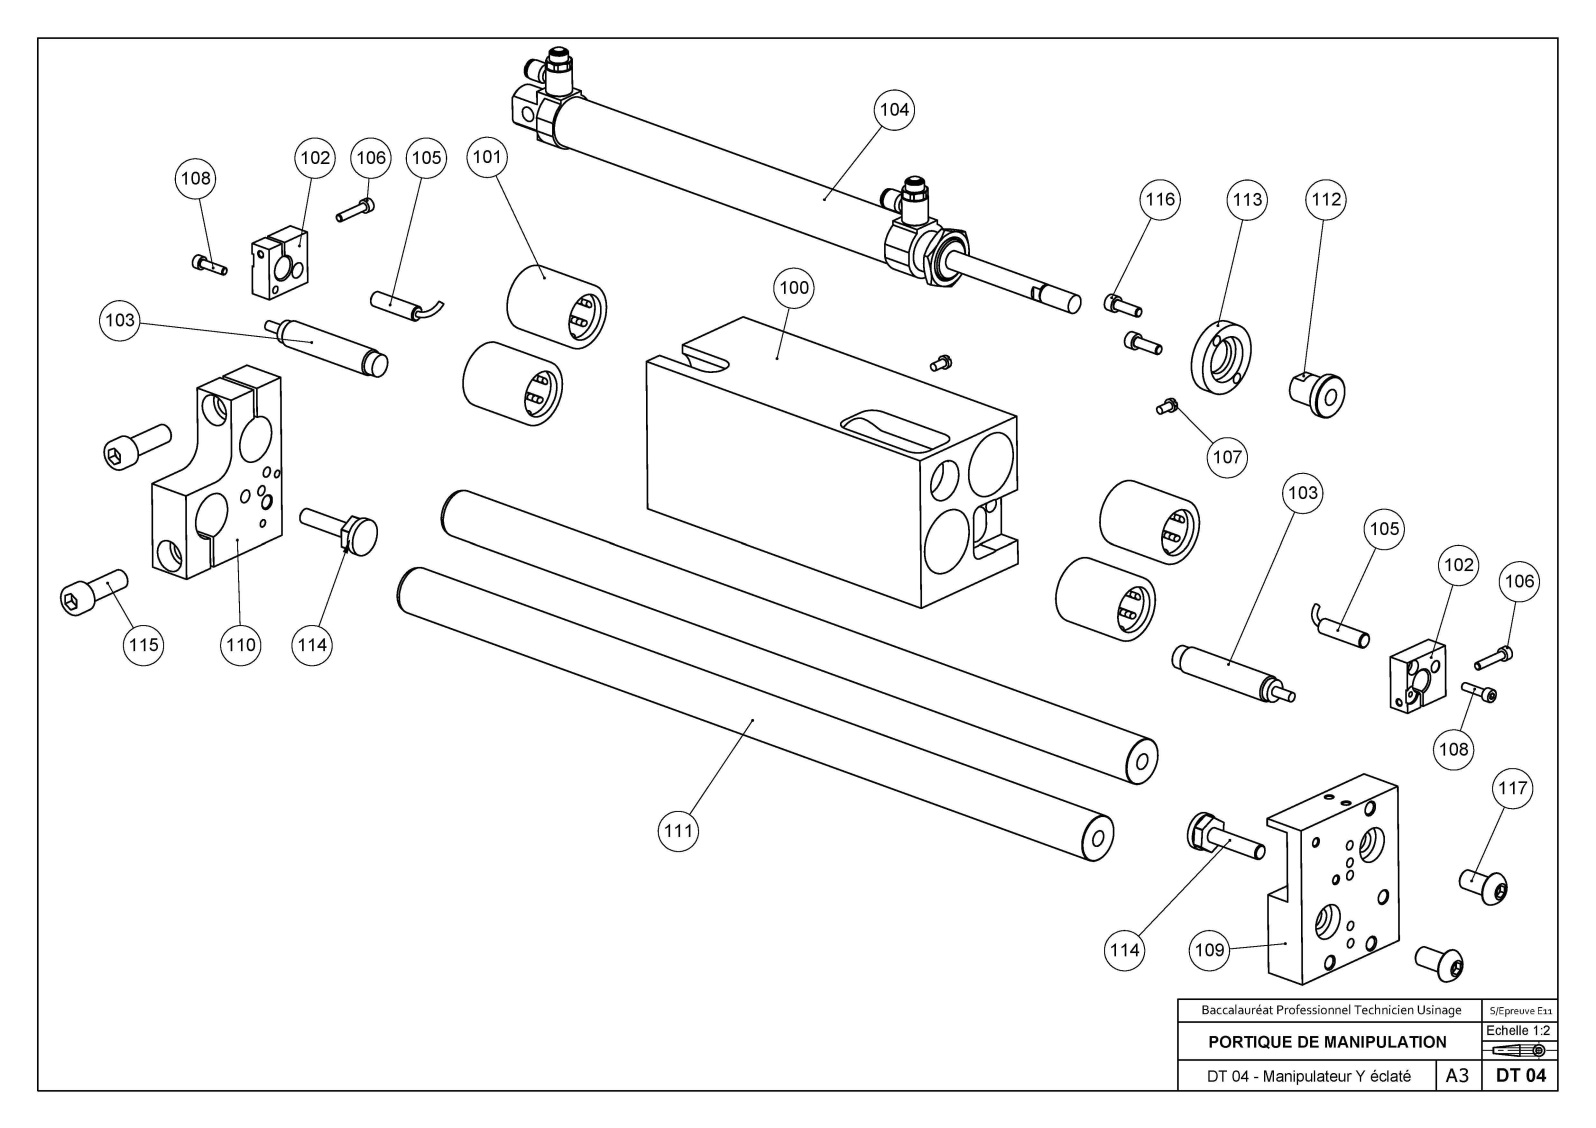
\includegraphics[width=\linewidth]{images/image173.jpeg}


\includegraphics[width=\linewidth]{images/image120.png}\textbf{SYSTÈME
D'ORIENTATION D'ANTENNE}

\emph{(\ul{Source :} Jérôme Letard)}


\includegraphics[width=\linewidth]{images/image156.png}
Niveau 2

\textbf{\ul{Objectifs de l'étude~:}}

\begin{itemize}
\item
  \textbf{Réaliser} le schéma cinématique du système d'orientation
  d'antenne.
\item
  \textbf{Déterminer} la durée d'alimentation du vérin électrique du
  système d'orientation d'antenne pour un déplacement donné.

  \begin{enumerate}
  \item
    
\includegraphics[width=\linewidth]{images/image174.emf}Mise
    en situation
  \end{enumerate}
\end{itemize}

x\textsubscript{0}

y\textsubscript{0}

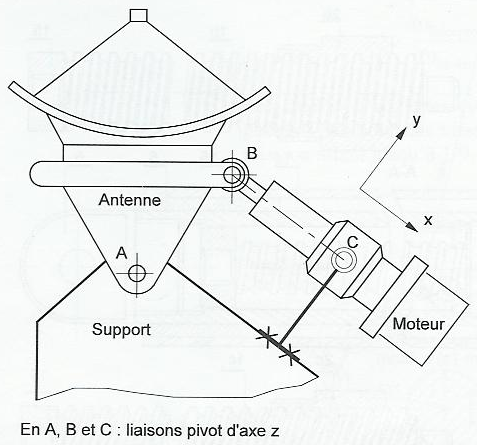
\includegraphics[width=\linewidth]{images/image175.png}Le
système d'orientation d'antenne ci-contre permet, grâce à une
télécommande, de régler à distance l'orientation de sa parabole afin
d'optimiser la réception des chaines de télévision.

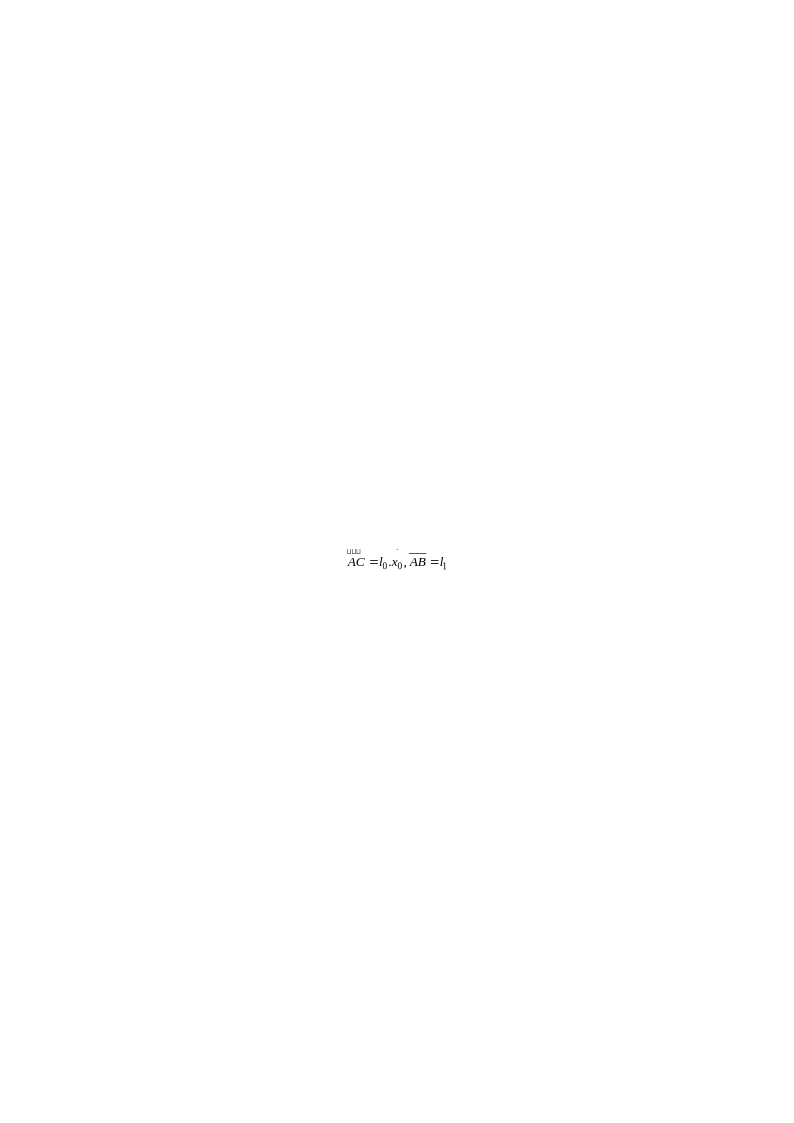
\includegraphics{images/image176.png}Pour cela, le moteur du vérin
électrique (type~: vis/écrou -- p\textsubscript{vis} = 2 mm/tr)) est
alimenté, de façon à faire rentrer ou sortir la tige et obtenir ainsi la
position de l'antenne désirée.

\begin{enumerate}
\setcounter{enumi}{1}
\item
  Modélisation du mécanisme
\end{enumerate}

\begin{enumerate}
\def\labelenumi{\arabic{enumi}.}
\item
  \textbf{Déterminer} les classes d'équivalence.
\item
  \textbf{Déterminer} la liaison entre la tige et le corps du vérin
  électrique.
\item
  \textbf{Établir} le graphe des liaisons.
\item
  \textbf{Justifier} que l'on peut se contenter du schéma cinématique
  dans le plan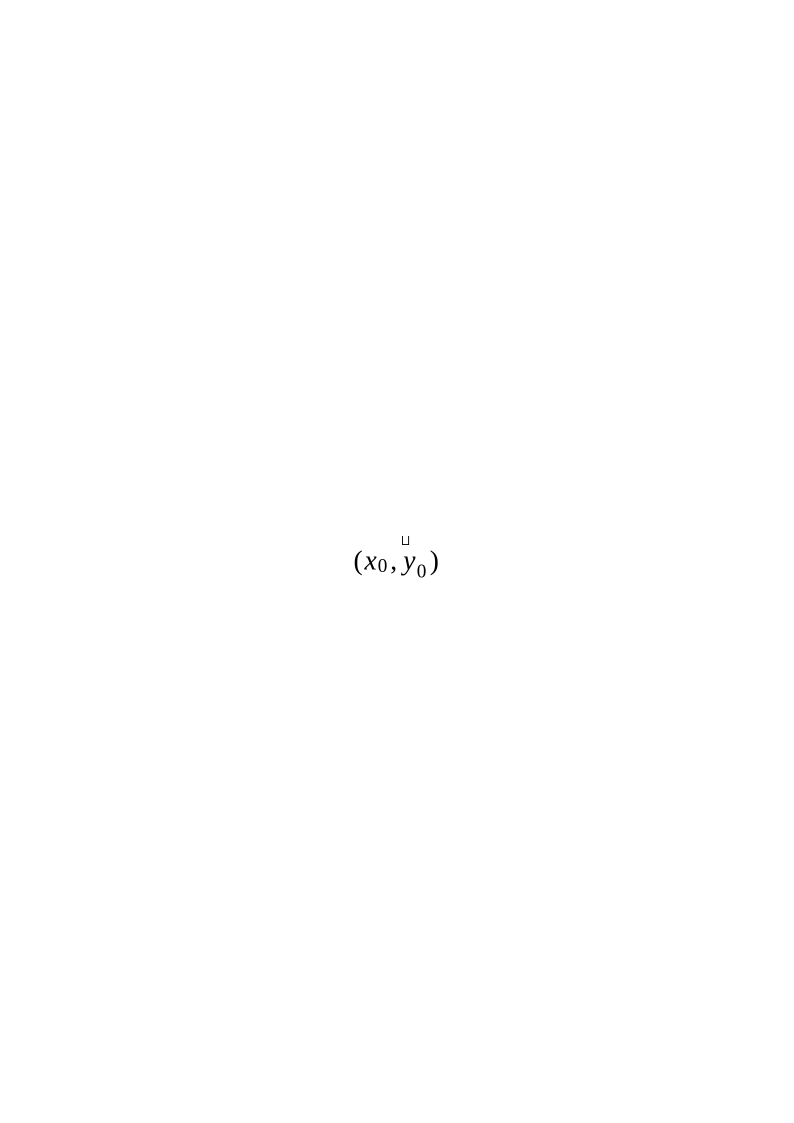
\includegraphics{images/image177.png}dans le cadre d'une
  étude cinématique. \textbf{Réaliser} ce schéma cinématique.

  \begin{enumerate}
  \item
    Détermination de la durée d'alimentation du vérin électrique
  \end{enumerate}
\item
  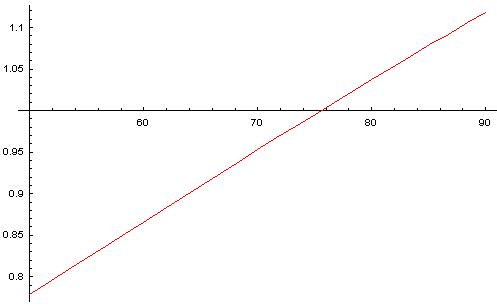
\includegraphics[width=\linewidth]{images/image178.jpeg}\textbf{Paramétrer}
  le système. \emph{On utilisera \textbf{d(t)} pour paramétrer le
  mouvement de la tige par rapport au corps du vérin,
  \textbf{α\textsubscript{1}(t)} pour paramétrer le mouvement de
  l'antenne par rapport au support et \textbf{α\textsubscript{2}(t)}
  pour paramétrer le mouvement du corps du vérin par rapport au
  support.}
\end{enumerate}

\textbf{\emph{d} =f(\emph{α\textsubscript{1})}}

α\textsubscript{1}(°)

\begin{enumerate}
\def\labelenumi{\arabic{enumi}.}
\setcounter{enumi}{5}
\item
  \textbf{Déterminer} la loi entrée sortie du mécanisme.
\item
  En utilisant le graphique de la loi entrée/sortie, \textbf{déterminer}
  la durée d'alimentation du vérin électrique pour faire pivoter
  l'antenne entre la position α\textsubscript{1} = 58° et
  α\textsubscript{1} =82°. \emph{On supposera que le moteur du vérin
  électrique tourne à une vitesse constante de 20 tr/s.}
\end{enumerate}

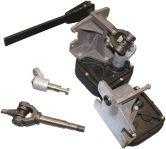
\includegraphics[width=\linewidth]{images/image179.jpeg}\textbf{BARRIERE
SINUSMATIC}


\includegraphics[width=\linewidth]{images/image156.png}
Niveau 3

\textbf{\ul{Objectif de l'étude~:}}

\begin{itemize}
\item
  \textbf{Modéliser} cinématiquement la barrière puis réaliser le schéma
  cinématique.

  \begin{enumerate}
  \item
    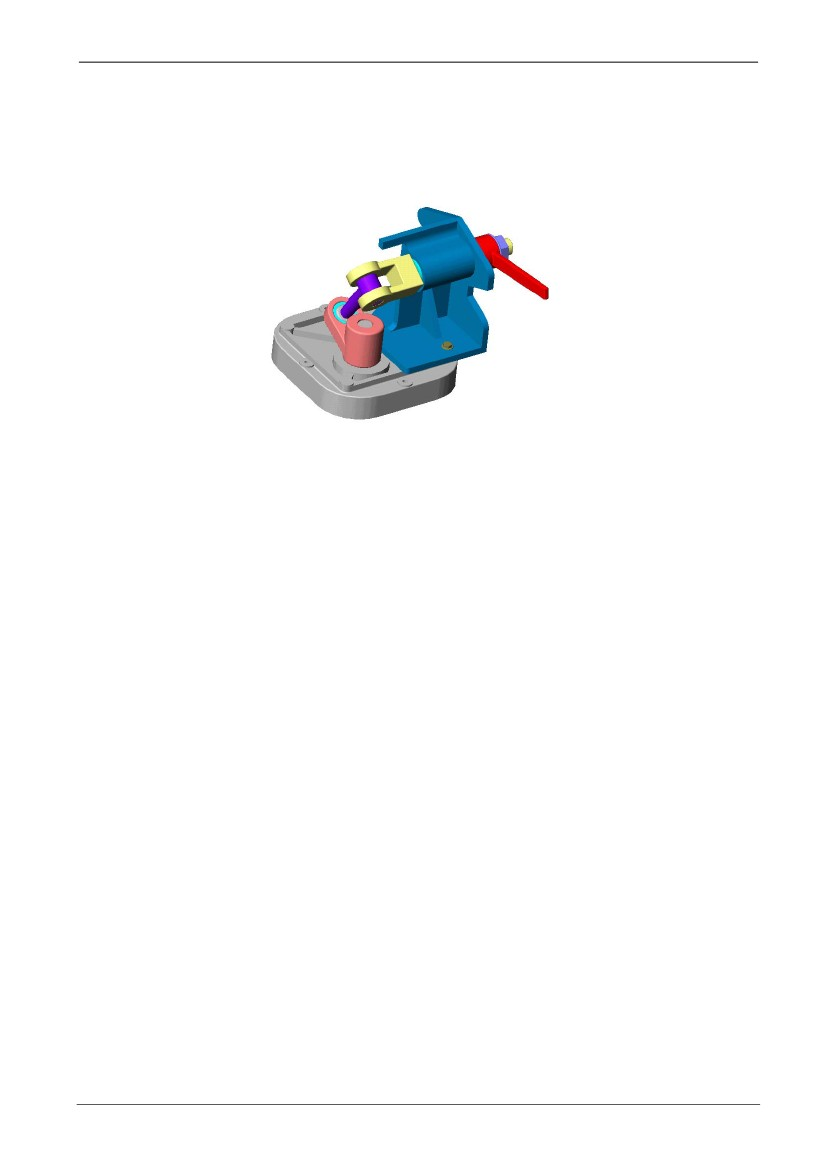
\includegraphics[width=\linewidth]{images/image180.jpeg}

    Mise en situation
  \end{enumerate}
\end{itemize}

\begin{quote}
Le système «~Sinusmatic~» permet l'ouverture ou la fermeture, dans un
plan verticale, des barrières de parking et de péages d'autoroute. Le
système proposé est commercialisé par la société ELLIPSE Industrie.
\end{quote}

Chaîne d'énergie

Moteur à courant continu

Réducteur à engrenages

SINUSMATIC

Barrière de parking

\begin{quote}
Ce système est commercialisé avec une motorisation par moteur à courant
continu commandé à distance par l'utilisateur de la barrière ou par le
système de gestion du péage.

La vitesse de rotation à la sortie de ce moteur est diminuée par un
réducteur à engrenages. L'arbre de sortie du réducteur est lié au
Sinusmatic par une liaison pivot réalisée par deux roulements à billes
(non représentés sur le dessin d'ensemble). Le Sinusmatic transforme la
rotation de l'arbre de sortie du réducteur en une rotation alternative
d'axe horizontale par l'utilisation d'un mécanisme dit sphérique.

Le plateau \textbf{7} en liaison encastrement avec l'arbre de sortie du
réducteur est animé d'un mouvement de rotation uniforme. Il est muni de
2 ergots qui lors de sa rotation viennent indiquer à la partie commande
sa position. A chaque demi-tour correspond une position haute ou basse
de la barrière. Le moteur a toujours le même sens de rotation.
\end{quote}

\emph{\ul{Remarque~:}} les pièces 4 sont deux roulements combinés à
aiguilles

\begin{enumerate}
\setcounter{enumi}{2}
\item
  Travail demandé
\end{enumerate}

\begin{enumerate}
\def\labelenumi{\arabic{enumi}.}
\item
  Sur le \emph{\textbf{document 1}}, Identifier les différents groupes
  cinématiques.
\item
  Réaliser le graphe des liaisons du système.
\item
  Réaliser le schéma cinématique minimal du système.
\end{enumerate}

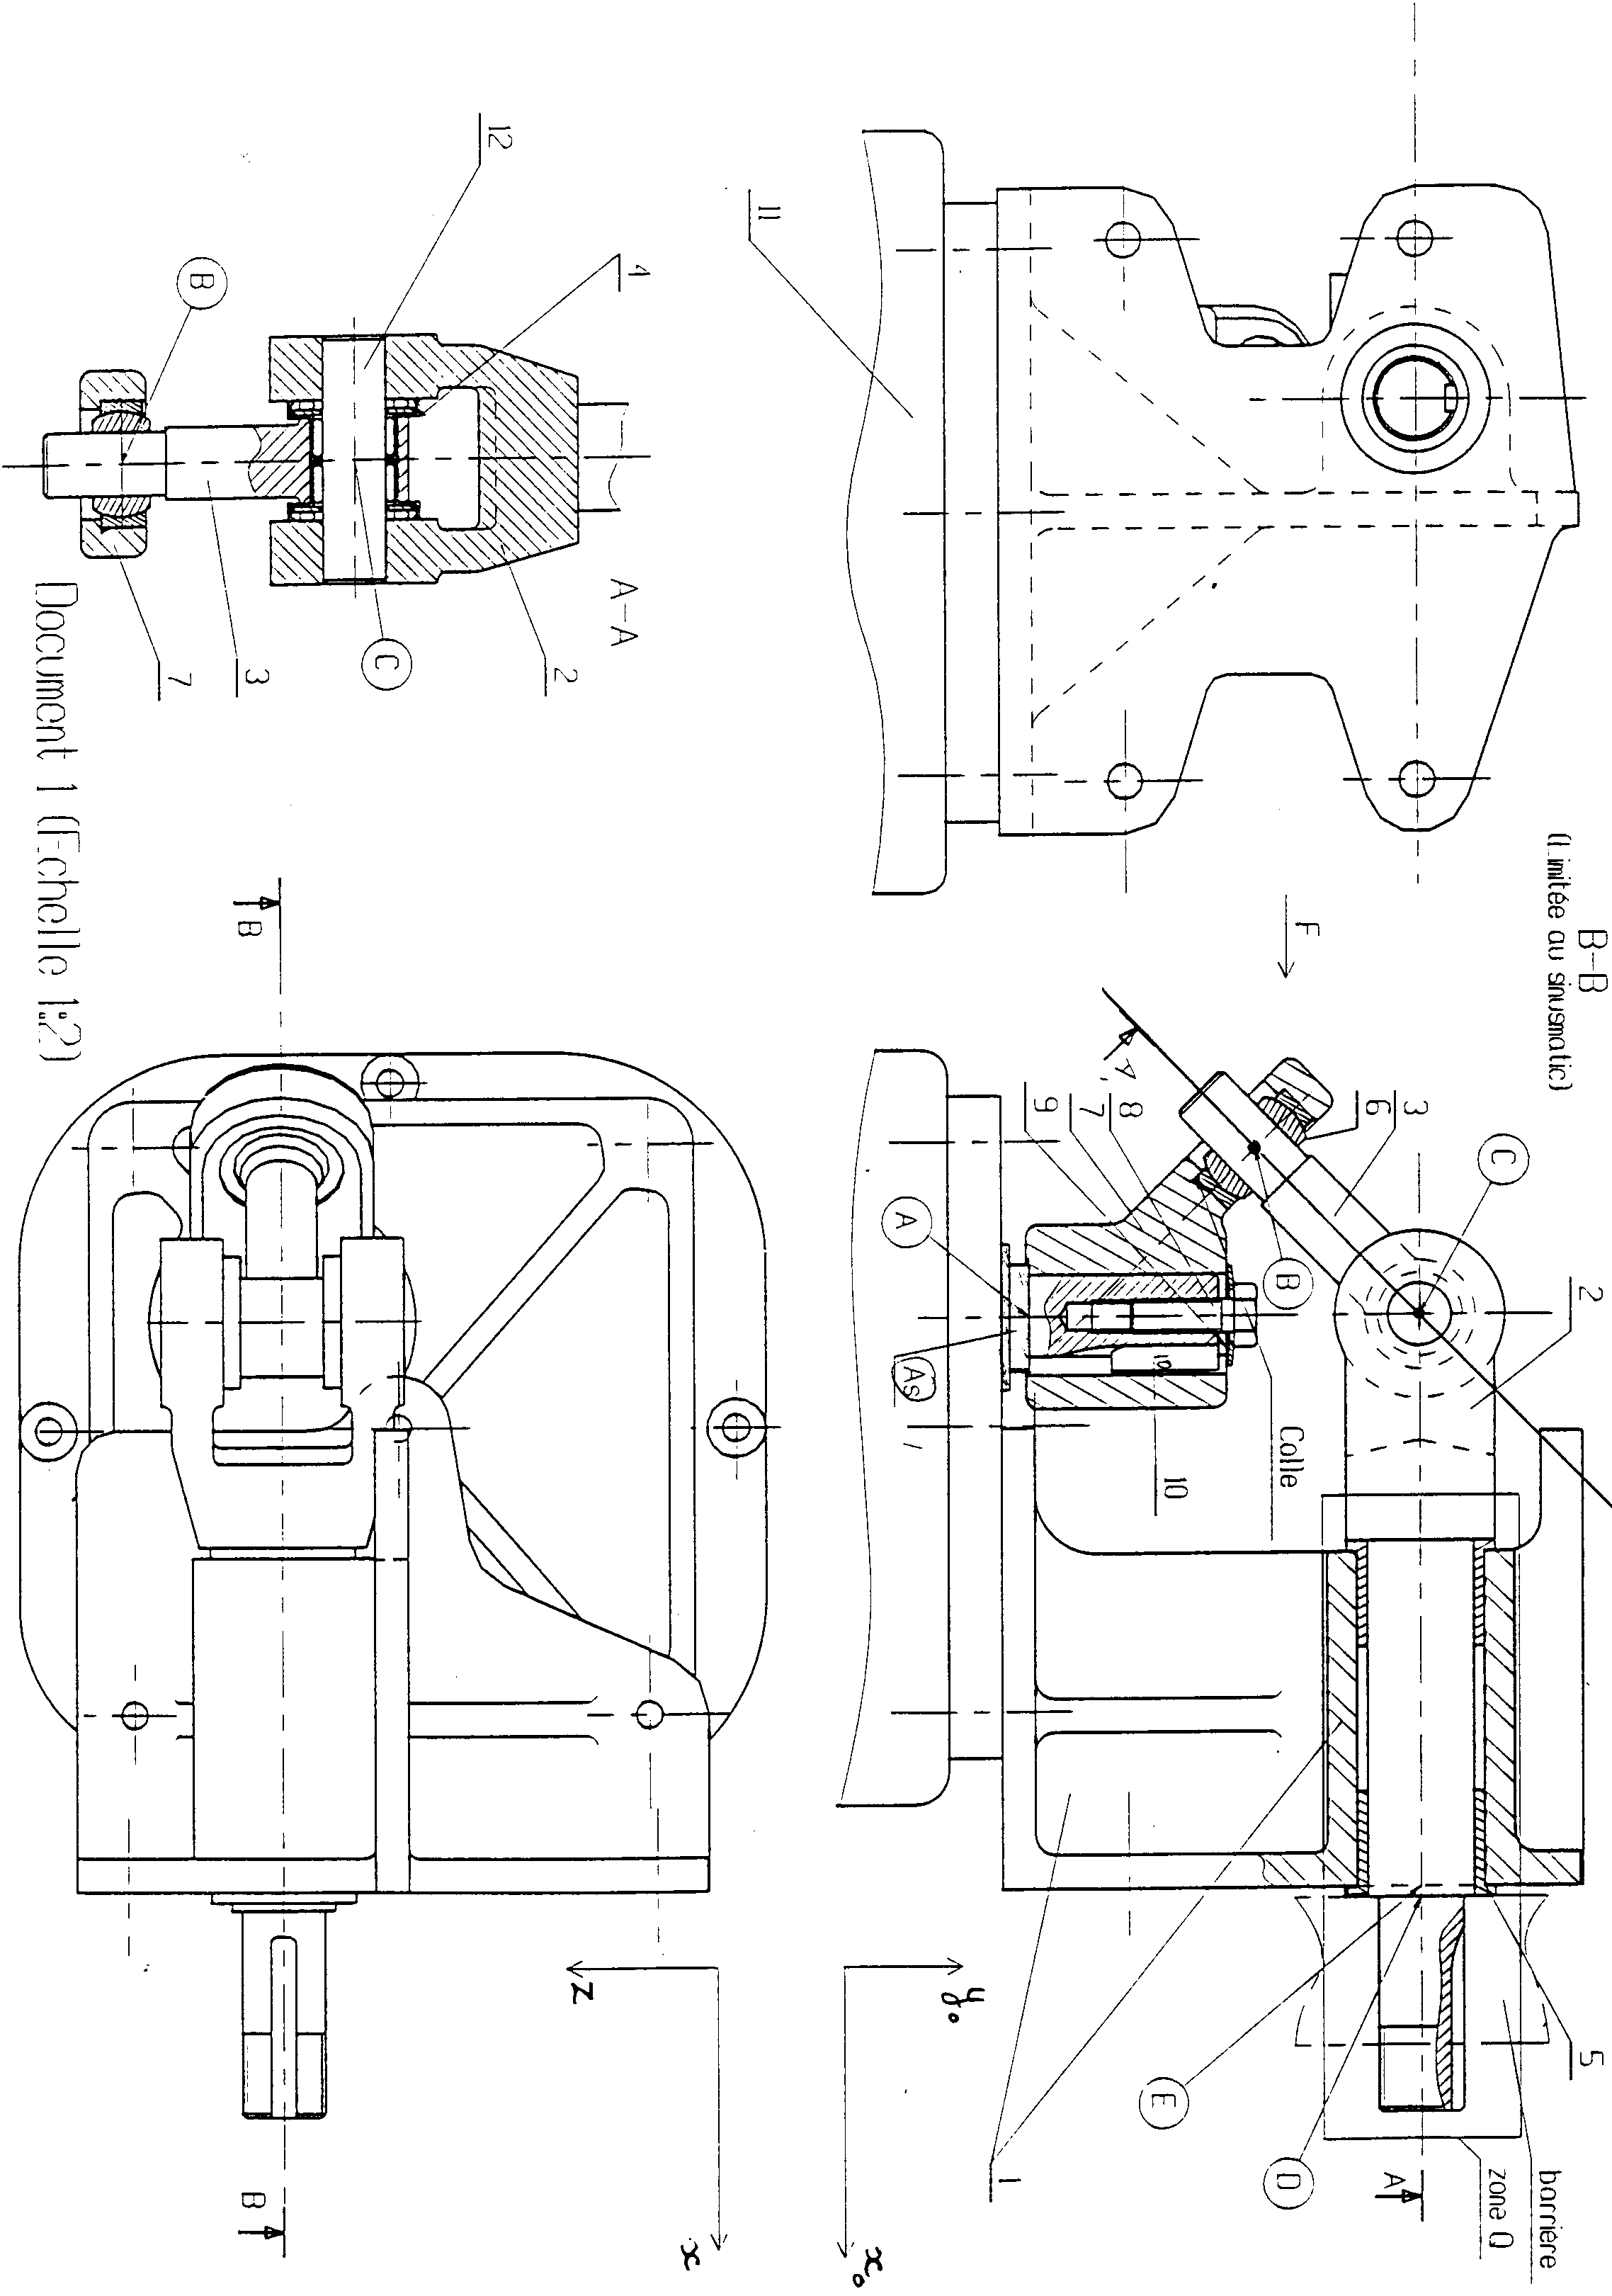
\includegraphics[width=\linewidth]{images/image181.png}

\textbf{SCIE SAUTEUSE}


\includegraphics[width=\linewidth]{images/image156.png}
Niveau 2

\textbf{\ul{Objectif de l'étude~:}}

\begin{itemize}
\item
  \textbf{Réaliser} la modélisation cinématique.
\end{itemize}

\includegraphics[width=\linewidth]{images/image182.png}

Le support étudié est un dispositif de transformation de mouvement (voir
figure ci-dessus) utilisé, par exemple, sur des scies sauteuses. Ce
dispositif permet de convertir un mouvement de rotation continue de
l'Arbre moteur en translation alternative du Porte lame. Il se classe
dans la famille des « transmetteurs - adaptateurs » au niveau de la
chaîne d'énergie.

\begin{enumerate}
\def\labelenumi{\arabic{enumi}.}
\item
  Réaliser le graphe de liaison.
\item
  Réaliser le schéma cinématique dans le plan (𝑂, 𝑦⃗ , 𝑧⃗ ) en couleur.
\item
  Réaliser le schéma cinématique 3D en couleur.
\end{enumerate}

\emph{\hfill\break
}

\includegraphics[width=\linewidth]{images/image183.png}\textbf{COMMANDE
DE SOUPAPE}

\includegraphics[width=\linewidth]{images/image156.png}
Niveau 3

\emph{(\ul{Source :} P. Provot)}

\textbf{\ul{Objectif de l'étude~:}}

\begin{itemize}
\item
  \textbf{Réaliser} le schéma cinématique de la commande de soupape.

  \begin{enumerate}
  \item
    Mise en situation
  \end{enumerate}
\end{itemize}

\includegraphics[width=\linewidth]{images/image184.png}Le
dessin en perspective représente le mécanisme de commande des quatre
soupapes d'un cylindre de moteur à explosion.

Pour ouvrir l'une des soupapes, la came \textbf{1} agit en A sur le
linguet \textbf{2} qui transmet une action mécanique à la soupape 6 par
l'intermédiaire de la tige \textbf{3}, du culbuteur \textbf{4}, du
poussoir réglable \textbf{5} en comprimant le ressort \textbf{7-8}.

L'examen de ce mécanisme montre que toutes ces pièces et les efforts
appliqués ont un plan de symétrie en commun.

\begin{enumerate}
\setcounter{enumi}{1}
\item
  Modélisation du mécanisme
\end{enumerate}

\begin{enumerate}
\def\labelenumi{\arabic{enumi}.}
\item
  Sur le \emph{\textbf{dessin d'ensemble,}} identifier les différents
  groupes cinématiques.
\item
  \textbf{Réaliser} le graphe des liaisons du système.
\item
  \textbf{Réaliser} le schéma cinématique du système dans le
  plan\includegraphics{images/image188.png}.
\end{enumerate}

\textbf{MODELISATION CINEMATIQUE DES MECANISMES}

\includegraphics[width=\linewidth]{images/image156.png}
Niveau 2

\begin{enumerate}
\item
  Capteur pneumatique
\end{enumerate}

Le capteur pneumatique représenté à l'aide de son dessin d'ensemble est
un composant pneumatique utilisé comme détecteur de fin de course d'un
vérin simple effet.

Lorsque la tige du vérin est en fin de course (tige totalement sortie),
son extrémité appuie sur le galet~\textbf{5}. Le levier \textbf{2}
pivote, ce qui a pour effet de déplacer le tiroir \textbf{6} vers le
bas. Lorsque le tiroir est déplacé verticalement vers le bas, l'air
comprimé admis dans le capteur pneumatique passe de l'orifice d'entrée à
l'orifice de sortie.

Cet air comprimé, dirigé vers le pré-actionneur, commande la coupure de
l'alimentation du vérin et provoquant ainsi la rentrée de la tige de
vérin grâce au ressort. Le capteur reprend alors sa position initiale :
le tiroir \textbf{6} remonte, poussé par le ressort \textbf{8}.

\includegraphics[width=\linewidth]{images/image189.png}

\textbf{Q1.} Indiquer le repère des pièces sur la perspective éclatée du
dessin d'ensemble.

\textbf{Q2.} Mettre en œuvre la démarche permettant d'obtenir le schéma
cinématique 2D dans le plan~\includegraphics{images/image190.png}

\textbf{Q3.} Réaliser le schéma cinématique 3D en prenant la même
orientation du capteur que celle sur la perspective.

\includegraphics[width=\linewidth]{images/image191.jpeg}

\includegraphics[width=\linewidth]{images/image192.png}Pince
de bras manipulateur

La pince représentée ci-dessous est une pince pneumatique située au bout
d'un bras manipulateur et permettant la préhension d'objets.

Sous l'action de l'air comprimé, le piston \textbf{8} se déplace et fait
pivoter les doigts \textbf{12} et \textbf{13}, par l'intermédiaire des
biellettes \textbf{11} et \textbf{14}.

\textbf{Q1.} Mettre en œuvre la démarche permettant d'obtenir le schéma
cinématique 2D dans le
plan~\protect\includegraphics{images/image193.png}

\protect\includegraphics{images/image194.emf}\protect\includegraphics[width=\linewidth]{images/image195.png}

\textbf{MODELISATION CINEMATIQUE DES MECANISMES}

\textbf{Q1.} Compléter le tableau ci-dessous.

- Indiquer la géométrie du contact réel entre les solides~: soit contact
ponctuel, soit contact linéique rectiligne (ligne) ou linéique annulaire
(arc de cercle), soit contact surfacique plan ou cylindrique ou
sphérique.

- Identifier le nombre de degrés de liberté.

- Donner le nom et les caractéristiques géométriques de la liaison
usuelle qui permet de modéliser le comportement cinématique d'un solide
par rapport à l'autre.

- Colorier (en bleu le plus clair et en rouge le plus foncé) les solides
sur les figures de la première colonne et indiquer en utilisant les
mêmes couleurs, les symboles correspondant à la liaison choisie.

- Indiquer la forme générale du torseur cinématique associé en précisant
les points où cette forme reste valable.

\begin{longtable}[]{@{}
  >{\raggedright\arraybackslash}p{(\columnwidth - 14\tabcolsep) * \real{0.0953}}
  >{\raggedright\arraybackslash}p{(\columnwidth - 14\tabcolsep) * \real{0.1153}}
  >{\raggedright\arraybackslash}p{(\columnwidth - 14\tabcolsep) * \real{0.1710}}
  >{\raggedright\arraybackslash}p{(\columnwidth - 14\tabcolsep) * \real{0.0790}}
  >{\raggedright\arraybackslash}p{(\columnwidth - 14\tabcolsep) * \real{0.0704}}
  >{\raggedright\arraybackslash}p{(\columnwidth - 14\tabcolsep) * \real{0.1376}}
  >{\raggedright\arraybackslash}p{(\columnwidth - 14\tabcolsep) * \real{0.1317}}
  >{\raggedright\arraybackslash}p{(\columnwidth - 14\tabcolsep) * \real{0.1996}}@{}}
\toprule\noalign{}
\endhead
\bottomrule\noalign{}
\endlastfoot
\includegraphics{images/image196.png}

O

\includegraphics{images/image197.png}

\includegraphics{images/image198.png} & \emph{\textbf{Géométrie du
contact}} & \emph{\textbf{Forme générale}}

\emph{\textbf{du Torseur cinématique}} & \emph{\textbf{Validité de la
forme générale}}

\emph{\textbf{du Torseur}} & \emph{\textbf{Degrés de liberté}} &
\emph{\textbf{Nom}} & \emph{\textbf{Représentation}}

\emph{\textbf{3D}}

\includegraphics{images/image199.png}

O

\includegraphics{images/image200.png}

\includegraphics{images/image201.png} & \emph{\textbf{Représentation
2D}}

\includegraphics{images/image202.png}

\includegraphics{images/image203.png}

\includegraphics{images/image204.png}

O

\includegraphics{images/image205.png}

\includegraphics{images/image206.png}

O \\
\includegraphics[width=\linewidth]{images/image207.jpeg} &
& & & & & & \\
\includegraphics[width=\linewidth]{images/image208.jpeg} &
& & & & & & \\
\includegraphics[width=\linewidth]{images/image209.jpeg}
& & & & & & & \\
\includegraphics[width=\linewidth]{images/image210.jpeg}
& & & & & & & \\
\includegraphics[width=\linewidth]{images/image211.jpeg}
& & & & & & & \\
\includegraphics[width=\linewidth]{images/image212.jpeg}
& & & & & & & \\
\includegraphics[width=\linewidth]{images/image213.jpeg}
& & & & & & & \\
\includegraphics[width=\linewidth]{images/image214.jpeg}
& & & & & & & \\
\includegraphics[width=\linewidth]{images/image39.jpeg}
& & & & & & & \\
\includegraphics[width=\linewidth]{images/image38.jpeg}
& & & & & & & \\
\end{longtable}

\emph{\hfill\break
}

\textbf{LIAISONS EQUIVALENTES}

\textbf{Q1.} Compléter le tableau ci-dessous en indiquant le nom et les
caractéristiques géométriques de la liaison située à gauche, de la
liaison située à droite et de la liaison équivalente aux deux
liaisons.(Le point caractéristique (centre, contact\ldots) de la liaison
de gauche sera nommé A et celui de la liaison de droite B).

\begin{longtable}[]{@{}
  >{\raggedright\arraybackslash}p{(\columnwidth - 8\tabcolsep) * \real{0.1622}}
  >{\raggedright\arraybackslash}p{(\columnwidth - 8\tabcolsep) * \real{0.2568}}
  >{\raggedright\arraybackslash}p{(\columnwidth - 8\tabcolsep) * \real{0.1783}}
  >{\raggedright\arraybackslash}p{(\columnwidth - 8\tabcolsep) * \real{0.2013}}
  >{\raggedright\arraybackslash}p{(\columnwidth - 8\tabcolsep) * \real{0.2014}}@{}}
\toprule\noalign{}
\begin{minipage}[b]{\linewidth}\raggedright
\end{minipage} & \begin{minipage}[b]{\linewidth}\raggedright
\textbf{Schéma}
\end{minipage} & \begin{minipage}[b]{\linewidth}\raggedright
\textbf{Liaison à gauche}
\end{minipage} & \begin{minipage}[b]{\linewidth}\raggedright
\textbf{Liaison à droite}
\end{minipage} & \begin{minipage}[b]{\linewidth}\raggedright
\textbf{Liaison équivalente}
\end{minipage} \\
\midrule\noalign{}
\endhead
\bottomrule\noalign{}
\endlastfoot
\multirow{8}{=}{\includegraphics{images/image215.png}

\includegraphics{images/image216.png}

\includegraphics{images/image217.png}} &
\includegraphics[width=\linewidth]{images/image218.jpeg}
& & & \\
&
\includegraphics[width=\linewidth]{images/image219.jpeg}
& & & \\
&
\includegraphics[width=\linewidth]{images/image220.emf}
& & & \\
&
\includegraphics[width=\linewidth]{images/image221.jpeg}
& & & \\
&
\includegraphics[width=\linewidth]{images/image222.jpeg}
& & & \\
&
\includegraphics[width=\linewidth]{images/image223.jpeg}
& & & \\
&
\includegraphics[width=\linewidth]{images/image224.jpeg}
& & & \\
&
\includegraphics[width=\linewidth]{images/image225.jpeg}
& & & \\
\multirow{3}{=}{\includegraphics{images/image226.png}

\includegraphics{images/image141.png}

\includegraphics{images/image142.png}} &
\includegraphics{images/image144.png} & & & \\
& \includegraphics{images/image227.png} & & & \\
& \includegraphics{images/image228.png} & & & \\
\end{longtable}

\textbf{20}

\textbf{\ul{Nom~:}}

\begin{enumerate}
\def\labelenumi{\arabic{enumi}.}
\item
  ~Quel sont les trois types de contact direct qu'il peut y avoir entre
  deux solides~? \emph{\textbf{(2 points)}}
\item
  ~Dans chacun des cas suivants, compléter les informations manquantes
  (symbole cinématique normalisé, nom de la liaison, tableau de
  mobilité). \emph{\textbf{Utiliser deux couleurs différentes pour les
  symboles cinématiques normalisés. (9 points)}}
\end{enumerate}

\begin{longtable}[]{@{}
  >{\raggedright\arraybackslash}p{(\columnwidth - 8\tabcolsep) * \real{0.1977}}
  >{\raggedright\arraybackslash}p{(\columnwidth - 8\tabcolsep) * \real{0.1518}}
  >{\raggedright\arraybackslash}p{(\columnwidth - 8\tabcolsep) * \real{0.2510}}
  >{\raggedright\arraybackslash}p{(\columnwidth - 8\tabcolsep) * \real{0.2701}}
  >{\raggedright\arraybackslash}p{(\columnwidth - 8\tabcolsep) * \real{0.1295}}@{}}
\toprule\noalign{}
\multirow{2}{=}{\begin{minipage}[b]{\linewidth}\raggedright
\textbf{Désignation de la liaison *}
\end{minipage}} &
\multicolumn{3}{>{\raggedright\arraybackslash}p{(\columnwidth - 8\tabcolsep) * \real{0.6729} + 4\tabcolsep}}{%
\begin{minipage}[b]{\linewidth}\raggedright
\textbf{Symbole}
\end{minipage}} &
\multirow{2}{=}{\begin{minipage}[b]{\linewidth}\raggedright
\textbf{Mobilités}
\end{minipage}} \\
&
\multicolumn{2}{>{\raggedright\arraybackslash}p{(\columnwidth - 8\tabcolsep) * \real{0.4028} + 2\tabcolsep}}{%
\begin{minipage}[b]{\linewidth}\raggedright
\textbf{Plan}
\end{minipage}} & \begin{minipage}[b]{\linewidth}\raggedright
\textbf{Spatial}
\end{minipage} \\
\midrule\noalign{}
\endhead
\bottomrule\noalign{}
\endlastfoot
sphère/plan de normale \(\overrightarrow{\text{z}}\)

(ponctuelle) &
\multicolumn{2}{>{\raggedright\arraybackslash}p{(\columnwidth - 8\tabcolsep) * \real{0.4028} + 2\tabcolsep}}{%
} & & \\
&
\includegraphics[width=\linewidth]{images/image50.jpeg}
&
\includegraphics[width=\linewidth]{images/image50.jpeg}
& & \\
& & &
\includegraphics[width=\linewidth]{images/image54.jpeg}
& \\
&
\multicolumn{2}{>{\raggedright\arraybackslash}p{(\columnwidth - 8\tabcolsep) * \real{0.4028} + 2\tabcolsep}}{%
\includegraphics[width=\linewidth]{images/image44.jpeg}}
&
\includegraphics[width=\linewidth]{images/image45.jpeg}
& \\
sphérique de centre O

(rotule) &
\multicolumn{2}{>{\raggedright\arraybackslash}p{(\columnwidth - 8\tabcolsep) * \real{0.4028} + 2\tabcolsep}}{%
} & & \\
pivot glissant d'axe
\(\left( \text{O,}\overrightarrow{\text{z}} \right)\) &
\includegraphics[width=\linewidth]{images/image58.jpeg}
& \includegraphics[width=\linewidth]{images/image58.jpeg}
& & \\
pivot d'axe \(\left( \text{O,}\overrightarrow{z} \right)\) & & & & \\
glissière de direction \(\overrightarrow{y}\) & & & & \\
& & &
\includegraphics[width=\linewidth]{images/image74.jpeg}
& \\
\end{longtable}

\begin{enumerate}
\def\labelenumi{\arabic{enumi}.}
\setcounter{enumi}{2}
\item
  ~Dans chacun des cas suivants, compléter les informations manquantes
  (symbole cinématique normalisé, nom de la liaison, tableau de
  mobilités). \emph{\textbf{(9 points)}}
\end{enumerate}

\emph{\textbf{Utiliser deux couleurs différentes pour les symboles
cinématique normalisés}}

Hélicoïdale d'axe
\includegraphics{images/image229.png}\includegraphics{images/image230.png}

\includegraphics{images/image76.png}

\textbf{T}

\textbf{R}

A

A

\includegraphics{images/image77.png}

\includegraphics{images/image76.png}

\includegraphics{images/image231.png}

\includegraphics{images/image232.png}

\includegraphics{images/image247.png}

1

0

1

E

\includegraphics{images/image233.png}

\textbf{T}

\textbf{R}

\includegraphics{images/image234.png}

\includegraphics{images/image235.png}

\includegraphics{images/image236.png}

\includegraphics{images/image237.png}

E

1

1

1

\includegraphics{images/image238.png}

\includegraphics{images/image239.png}

Glissière de direction
\includegraphics{images/image240.png}\includegraphics{images/image230.png}

\includegraphics{images/image241.png}

\textbf{T}

\textbf{R}

\includegraphics{images/image239.png}

\textbf{T}

\textbf{R}

O

0

1

0

1

0

1

O

\includegraphics{images/image248.png}

\textbf{T}

\textbf{R}

\includegraphics{images/image249.png}

\includegraphics{images/image250.png}

\includegraphics{images/image251.png}

\includegraphics{images/image252.png}
